
\documentclass[10pt]{article} % For LaTeX2e
% \usepackage{tmlr}
% If accepted, instead use the following line for the camera-ready submission:
% \usepackage[accepted]{tmlr}
% To de-anonymize and remove mentions to TMLR (for example for posting to preprint servers), instead use the following:
\usepackage[preprint]{tmlr}

% Optional math commands from https://github.com/goodfeli/dlbook_notation.
% --- begin math_commands.tex ---
%%%%% NEW MATH DEFINITIONS %%%%%

\usepackage{amsmath,amsfonts,bm}

% Mark sections of captions for referring to divisions of figures
\newcommand{\figleft}{{\em (Left)}}
\newcommand{\figcenter}{{\em (Center)}}
\newcommand{\figright}{{\em (Right)}}
\newcommand{\figtop}{{\em (Top)}}
\newcommand{\figbottom}{{\em (Bottom)}}
\newcommand{\captiona}{{\em (a)}}
\newcommand{\captionb}{{\em (b)}}
\newcommand{\captionc}{{\em (c)}}
\newcommand{\captiond}{{\em (d)}}

% Highlight a newly defined term
\newcommand{\newterm}[1]{{\bf #1}}


% Figure reference, lower-case.
\def\figref#1{figure~\ref{#1}}
% Figure reference, capital. For start of sentence
\def\Figref#1{Figure~\ref{#1}}
\def\twofigref#1#2{figures \ref{#1} and \ref{#2}}
\def\quadfigref#1#2#3#4{figures \ref{#1}, \ref{#2}, \ref{#3} and \ref{#4}}
% Section reference, lower-case.
\def\secref#1{section~\ref{#1}}
% Section reference, capital.
\def\Secref#1{Section~\ref{#1}}
% Reference to two sections.
\def\twosecrefs#1#2{sections \ref{#1} and \ref{#2}}
% Reference to three sections.
\def\secrefs#1#2#3{sections \ref{#1}, \ref{#2} and \ref{#3}}
% Reference to an equation, lower-case.
\def\eqref#1{equation~\ref{#1}}
% Reference to an equation, upper case
\def\Eqref#1{Equation~\ref{#1}}
% A raw reference to an equation---avoid using if possible
\def\plaineqref#1{\ref{#1}}
% Reference to a chapter, lower-case.
\def\chapref#1{chapter~\ref{#1}}
% Reference to an equation, upper case.
\def\Chapref#1{Chapter~\ref{#1}}
% Reference to a range of chapters
\def\rangechapref#1#2{chapters\ref{#1}--\ref{#2}}
% Reference to an algorithm, lower-case.
\def\algref#1{algorithm~\ref{#1}}
% Reference to an algorithm, upper case.
\def\Algref#1{Algorithm~\ref{#1}}
\def\twoalgref#1#2{algorithms \ref{#1} and \ref{#2}}
\def\Twoalgref#1#2{Algorithms \ref{#1} and \ref{#2}}
% Reference to a part, lower case
\def\partref#1{part~\ref{#1}}
% Reference to a part, upper case
\def\Partref#1{Part~\ref{#1}}
\def\twopartref#1#2{parts \ref{#1} and \ref{#2}}

\def\ceil#1{\lceil #1 \rceil}
\def\floor#1{\lfloor #1 \rfloor}
\def\1{\bm{1}}
\newcommand{\train}{\mathcal{D}}
\newcommand{\valid}{\mathcal{D_{\mathrm{valid}}}}
\newcommand{\test}{\mathcal{D_{\mathrm{test}}}}

\def\eps{{\epsilon}}


% Random variables
\def\reta{{\textnormal{$\eta$}}}
\def\ra{{\textnormal{a}}}
\def\rb{{\textnormal{b}}}
\def\rc{{\textnormal{c}}}
\def\rd{{\textnormal{d}}}
\def\re{{\textnormal{e}}}
\def\rf{{\textnormal{f}}}
\def\rg{{\textnormal{g}}}
\def\rh{{\textnormal{h}}}
\def\ri{{\textnormal{i}}}
\def\rj{{\textnormal{j}}}
\def\rk{{\textnormal{k}}}
\def\rl{{\textnormal{l}}}
% rm is already a command, just don't name any random variables m
\def\rn{{\textnormal{n}}}
\def\ro{{\textnormal{o}}}
\def\rp{{\textnormal{p}}}
\def\rq{{\textnormal{q}}}
\def\rr{{\textnormal{r}}}
\def\rs{{\textnormal{s}}}
\def\rt{{\textnormal{t}}}
\def\ru{{\textnormal{u}}}
\def\rv{{\textnormal{v}}}
\def\rw{{\textnormal{w}}}
\def\rx{{\textnormal{x}}}
\def\ry{{\textnormal{y}}}
\def\rz{{\textnormal{z}}}

% Random vectors
\def\rvepsilon{{\mathbf{\epsilon}}}
\def\rvtheta{{\mathbf{\theta}}}
\def\rva{{\mathbf{a}}}
\def\rvb{{\mathbf{b}}}
\def\rvc{{\mathbf{c}}}
\def\rvd{{\mathbf{d}}}
\def\rve{{\mathbf{e}}}
\def\rvf{{\mathbf{f}}}
\def\rvg{{\mathbf{g}}}
\def\rvh{{\mathbf{h}}}
\def\rvu{{\mathbf{i}}}
\def\rvj{{\mathbf{j}}}
\def\rvk{{\mathbf{k}}}
\def\rvl{{\mathbf{l}}}
\def\rvm{{\mathbf{m}}}
\def\rvn{{\mathbf{n}}}
\def\rvo{{\mathbf{o}}}
\def\rvp{{\mathbf{p}}}
\def\rvq{{\mathbf{q}}}
\def\rvr{{\mathbf{r}}}
\def\rvs{{\mathbf{s}}}
\def\rvt{{\mathbf{t}}}
\def\rvu{{\mathbf{u}}}
\def\rvv{{\mathbf{v}}}
\def\rvw{{\mathbf{w}}}
\def\rvx{{\mathbf{x}}}
\def\rvy{{\mathbf{y}}}
\def\rvz{{\mathbf{z}}}

% Elements of random vectors
\def\erva{{\textnormal{a}}}
\def\ervb{{\textnormal{b}}}
\def\ervc{{\textnormal{c}}}
\def\ervd{{\textnormal{d}}}
\def\erve{{\textnormal{e}}}
\def\ervf{{\textnormal{f}}}
\def\ervg{{\textnormal{g}}}
\def\ervh{{\textnormal{h}}}
\def\ervi{{\textnormal{i}}}
\def\ervj{{\textnormal{j}}}
\def\ervk{{\textnormal{k}}}
\def\ervl{{\textnormal{l}}}
\def\ervm{{\textnormal{m}}}
\def\ervn{{\textnormal{n}}}
\def\ervo{{\textnormal{o}}}
\def\ervp{{\textnormal{p}}}
\def\ervq{{\textnormal{q}}}
\def\ervr{{\textnormal{r}}}
\def\ervs{{\textnormal{s}}}
\def\ervt{{\textnormal{t}}}
\def\ervu{{\textnormal{u}}}
\def\ervv{{\textnormal{v}}}
\def\ervw{{\textnormal{w}}}
\def\ervx{{\textnormal{x}}}
\def\ervy{{\textnormal{y}}}
\def\ervz{{\textnormal{z}}}

% Random matrices
\def\rmA{{\mathbf{A}}}
\def\rmB{{\mathbf{B}}}
\def\rmC{{\mathbf{C}}}
\def\rmD{{\mathbf{D}}}
\def\rmE{{\mathbf{E}}}
\def\rmF{{\mathbf{F}}}
\def\rmG{{\mathbf{G}}}
\def\rmH{{\mathbf{H}}}
\def\rmI{{\mathbf{I}}}
\def\rmJ{{\mathbf{J}}}
\def\rmK{{\mathbf{K}}}
\def\rmL{{\mathbf{L}}}
\def\rmM{{\mathbf{M}}}
\def\rmN{{\mathbf{N}}}
\def\rmO{{\mathbf{O}}}
\def\rmP{{\mathbf{P}}}
\def\rmQ{{\mathbf{Q}}}
\def\rmR{{\mathbf{R}}}
\def\rmS{{\mathbf{S}}}
\def\rmT{{\mathbf{T}}}
\def\rmU{{\mathbf{U}}}
\def\rmV{{\mathbf{V}}}
\def\rmW{{\mathbf{W}}}
\def\rmX{{\mathbf{X}}}
\def\rmY{{\mathbf{Y}}}
\def\rmZ{{\mathbf{Z}}}

% Elements of random matrices
\def\ermA{{\textnormal{A}}}
\def\ermB{{\textnormal{B}}}
\def\ermC{{\textnormal{C}}}
\def\ermD{{\textnormal{D}}}
\def\ermE{{\textnormal{E}}}
\def\ermF{{\textnormal{F}}}
\def\ermG{{\textnormal{G}}}
\def\ermH{{\textnormal{H}}}
\def\ermI{{\textnormal{I}}}
\def\ermJ{{\textnormal{J}}}
\def\ermK{{\textnormal{K}}}
\def\ermL{{\textnormal{L}}}
\def\ermM{{\textnormal{M}}}
\def\ermN{{\textnormal{N}}}
\def\ermO{{\textnormal{O}}}
\def\ermP{{\textnormal{P}}}
\def\ermQ{{\textnormal{Q}}}
\def\ermR{{\textnormal{R}}}
\def\ermS{{\textnormal{S}}}
\def\ermT{{\textnormal{T}}}
\def\ermU{{\textnormal{U}}}
\def\ermV{{\textnormal{V}}}
\def\ermW{{\textnormal{W}}}
\def\ermX{{\textnormal{X}}}
\def\ermY{{\textnormal{Y}}}
\def\ermZ{{\textnormal{Z}}}

% Vectors
\def\vzero{{\bm{0}}}
\def\vone{{\bm{1}}}
\def\vmu{{\bm{\mu}}}
\def\vtheta{{\bm{\theta}}}
\def\va{{\bm{a}}}
\def\vb{{\bm{b}}}
\def\vc{{\bm{c}}}
\def\vd{{\bm{d}}}
\def\ve{{\bm{e}}}
\def\vf{{\bm{f}}}
\def\vg{{\bm{g}}}
\def\vh{{\bm{h}}}
\def\vi{{\bm{i}}}
\def\vj{{\bm{j}}}
\def\vk{{\bm{k}}}
\def\vl{{\bm{l}}}
\def\vm{{\bm{m}}}
\def\vn{{\bm{n}}}
\def\vo{{\bm{o}}}
\def\vp{{\bm{p}}}
\def\vq{{\bm{q}}}
\def\vr{{\bm{r}}}
\def\vs{{\bm{s}}}
\def\vt{{\bm{t}}}
\def\vu{{\bm{u}}}
\def\vv{{\bm{v}}}
\def\vw{{\bm{w}}}
\def\vx{{\bm{x}}}
\def\vy{{\bm{y}}}
\def\vz{{\bm{z}}}

% Elements of vectors
\def\evalpha{{\alpha}}
\def\evbeta{{\beta}}
\def\evepsilon{{\epsilon}}
\def\evlambda{{\lambda}}
\def\evomega{{\omega}}
\def\evmu{{\mu}}
\def\evpsi{{\psi}}
\def\evsigma{{\sigma}}
\def\evtheta{{\theta}}
\def\eva{{a}}
\def\evb{{b}}
\def\evc{{c}}
\def\evd{{d}}
\def\eve{{e}}
\def\evf{{f}}
\def\evg{{g}}
\def\evh{{h}}
\def\evi{{i}}
\def\evj{{j}}
\def\evk{{k}}
\def\evl{{l}}
\def\evm{{m}}
\def\evn{{n}}
\def\evo{{o}}
\def\evp{{p}}
\def\evq{{q}}
\def\evr{{r}}
\def\evs{{s}}
\def\evt{{t}}
\def\evu{{u}}
\def\evv{{v}}
\def\evw{{w}}
\def\evx{{x}}
\def\evy{{y}}
\def\evz{{z}}

% Matrix
\def\mA{{\bm{A}}}
\def\mB{{\bm{B}}}
\def\mC{{\bm{C}}}
\def\mD{{\bm{D}}}
\def\mE{{\bm{E}}}
\def\mF{{\bm{F}}}
\def\mG{{\bm{G}}}
\def\mH{{\bm{H}}}
\def\mI{{\bm{I}}}
\def\mJ{{\bm{J}}}
\def\mK{{\bm{K}}}
\def\mL{{\bm{L}}}
\def\mM{{\bm{M}}}
\def\mN{{\bm{N}}}
\def\mO{{\bm{O}}}
\def\mP{{\bm{P}}}
\def\mQ{{\bm{Q}}}
\def\mR{{\bm{R}}}
\def\mS{{\bm{S}}}
\def\mT{{\bm{T}}}
\def\mU{{\bm{U}}}
\def\mV{{\bm{V}}}
\def\mW{{\bm{W}}}
\def\mX{{\bm{X}}}
\def\mY{{\bm{Y}}}
\def\mZ{{\bm{Z}}}
\def\mBeta{{\bm{\beta}}}
\def\mPhi{{\bm{\Phi}}}
\def\mLambda{{\bm{\Lambda}}}
\def\mSigma{{\bm{\Sigma}}}

% Tensor
\DeclareMathAlphabet{\mathsfit}{\encodingdefault}{\sfdefault}{m}{sl}
\SetMathAlphabet{\mathsfit}{bold}{\encodingdefault}{\sfdefault}{bx}{n}
\newcommand{\tens}[1]{\bm{\mathsfit{#1}}}
\def\tA{{\tens{A}}}
\def\tB{{\tens{B}}}
\def\tC{{\tens{C}}}
\def\tD{{\tens{D}}}
\def\tE{{\tens{E}}}
\def\tF{{\tens{F}}}
\def\tG{{\tens{G}}}
\def\tH{{\tens{H}}}
\def\tI{{\tens{I}}}
\def\tJ{{\tens{J}}}
\def\tK{{\tens{K}}}
\def\tL{{\tens{L}}}
\def\tM{{\tens{M}}}
\def\tN{{\tens{N}}}
\def\tO{{\tens{O}}}
\def\tP{{\tens{P}}}
\def\tQ{{\tens{Q}}}
\def\tR{{\tens{R}}}
\def\tS{{\tens{S}}}
\def\tT{{\tens{T}}}
\def\tU{{\tens{U}}}
\def\tV{{\tens{V}}}
\def\tW{{\tens{W}}}
\def\tX{{\tens{X}}}
\def\tY{{\tens{Y}}}
\def\tZ{{\tens{Z}}}


% Graph
\def\gA{{\mathcal{A}}}
\def\gB{{\mathcal{B}}}
\def\gC{{\mathcal{C}}}
\def\gD{{\mathcal{D}}}
\def\gE{{\mathcal{E}}}
\def\gF{{\mathcal{F}}}
\def\gG{{\mathcal{G}}}
\def\gH{{\mathcal{H}}}
\def\gI{{\mathcal{I}}}
\def\gJ{{\mathcal{J}}}
\def\gK{{\mathcal{K}}}
\def\gL{{\mathcal{L}}}
\def\gM{{\mathcal{M}}}
\def\gN{{\mathcal{N}}}
\def\gO{{\mathcal{O}}}
\def\gP{{\mathcal{P}}}
\def\gQ{{\mathcal{Q}}}
\def\gR{{\mathcal{R}}}
\def\gS{{\mathcal{S}}}
\def\gT{{\mathcal{T}}}
\def\gU{{\mathcal{U}}}
\def\gV{{\mathcal{V}}}
\def\gW{{\mathcal{W}}}
\def\gX{{\mathcal{X}}}
\def\gY{{\mathcal{Y}}}
\def\gZ{{\mathcal{Z}}}

% Sets
\def\sA{{\mathbb{A}}}
\def\sB{{\mathbb{B}}}
\def\sC{{\mathbb{C}}}
\def\sD{{\mathbb{D}}}
% Don't use a set called E, because this would be the same as our symbol
% for expectation.
\def\sF{{\mathbb{F}}}
\def\sG{{\mathbb{G}}}
\def\sH{{\mathbb{H}}}
\def\sI{{\mathbb{I}}}
\def\sJ{{\mathbb{J}}}
\def\sK{{\mathbb{K}}}
\def\sL{{\mathbb{L}}}
\def\sM{{\mathbb{M}}}
\def\sN{{\mathbb{N}}}
\def\sO{{\mathbb{O}}}
\def\sP{{\mathbb{P}}}
\def\sQ{{\mathbb{Q}}}
\def\sR{{\mathbb{R}}}
\def\sS{{\mathbb{S}}}
\def\sT{{\mathbb{T}}}
\def\sU{{\mathbb{U}}}
\def\sV{{\mathbb{V}}}
\def\sW{{\mathbb{W}}}
\def\sX{{\mathbb{X}}}
\def\sY{{\mathbb{Y}}}
\def\sZ{{\mathbb{Z}}}

% Entries of a matrix
\def\emLambda{{\Lambda}}
\def\emA{{A}}
\def\emB{{B}}
\def\emC{{C}}
\def\emD{{D}}
\def\emE{{E}}
\def\emF{{F}}
\def\emG{{G}}
\def\emH{{H}}
\def\emI{{I}}
\def\emJ{{J}}
\def\emK{{K}}
\def\emL{{L}}
\def\emM{{M}}
\def\emN{{N}}
\def\emO{{O}}
\def\emP{{P}}
\def\emQ{{Q}}
\def\emR{{R}}
\def\emS{{S}}
\def\emT{{T}}
\def\emU{{U}}
\def\emV{{V}}
\def\emW{{W}}
\def\emX{{X}}
\def\emY{{Y}}
\def\emZ{{Z}}
\def\emSigma{{\Sigma}}

% entries of a tensor
% Same font as tensor, without \bm wrapper
\newcommand{\etens}[1]{\mathsfit{#1}}
\def\etLambda{{\etens{\Lambda}}}
\def\etA{{\etens{A}}}
\def\etB{{\etens{B}}}
\def\etC{{\etens{C}}}
\def\etD{{\etens{D}}}
\def\etE{{\etens{E}}}
\def\etF{{\etens{F}}}
\def\etG{{\etens{G}}}
\def\etH{{\etens{H}}}
\def\etI{{\etens{I}}}
\def\etJ{{\etens{J}}}
\def\etK{{\etens{K}}}
\def\etL{{\etens{L}}}
\def\etM{{\etens{M}}}
\def\etN{{\etens{N}}}
\def\etO{{\etens{O}}}
\def\etP{{\etens{P}}}
\def\etQ{{\etens{Q}}}
\def\etR{{\etens{R}}}
\def\etS{{\etens{S}}}
\def\etT{{\etens{T}}}
\def\etU{{\etens{U}}}
\def\etV{{\etens{V}}}
\def\etW{{\etens{W}}}
\def\etX{{\etens{X}}}
\def\etY{{\etens{Y}}}
\def\etZ{{\etens{Z}}}

% The true underlying data generating distribution
\newcommand{\pdata}{p_{\rm{data}}}
% The empirical distribution defined by the training set
\newcommand{\ptrain}{\hat{p}_{\rm{data}}}
\newcommand{\Ptrain}{\hat{P}_{\rm{data}}}
% The model distribution
\newcommand{\pmodel}{p_{\rm{model}}}
\newcommand{\Pmodel}{P_{\rm{model}}}
\newcommand{\ptildemodel}{\tilde{p}_{\rm{model}}}
% Stochastic autoencoder distributions
\newcommand{\pencode}{p_{\rm{encoder}}}
\newcommand{\pdecode}{p_{\rm{decoder}}}
\newcommand{\precons}{p_{\rm{reconstruct}}}

\newcommand{\laplace}{\mathrm{Laplace}} % Laplace distribution

\newcommand{\E}{\mathbb{E}}
\newcommand{\Ls}{\mathcal{L}}
\newcommand{\R}{\mathbb{R}}
\newcommand{\emp}{\tilde{p}}
\newcommand{\lr}{\alpha}
\newcommand{\reg}{\lambda}
\newcommand{\rect}{\mathrm{rectifier}}
\newcommand{\softmax}{\mathrm{softmax}}
\newcommand{\sigmoid}{\sigma}
\newcommand{\softplus}{\zeta}
\newcommand{\KL}{D_{\mathrm{KL}}}
\newcommand{\Var}{\mathrm{Var}}
\newcommand{\standarderror}{\mathrm{SE}}
\newcommand{\Cov}{\mathrm{Cov}}
% Wolfram Mathworld says $L^2$ is for function spaces and $\ell^2$ is for vectors
% But then they seem to use $L^2$ for vectors throughout the site, and so does
% wikipedia.
\newcommand{\normlzero}{L^0}
\newcommand{\normlone}{L^1}
\newcommand{\normltwo}{L^2}
\newcommand{\normlp}{L^p}
\newcommand{\normmax}{L^\infty}

\newcommand{\parents}{Pa} % See usage in notation.tex. Chosen to match Daphne's book.

\DeclareMathOperator*{\argmax}{arg\,max}
\DeclareMathOperator*{\argmin}{arg\,min}

\DeclareMathOperator{\sign}{sign}
\DeclareMathOperator{\Tr}{Tr}
\let\ab\allowbreak
% --- end math_commands.tex ---

\usepackage{caption}
\usepackage{algorithm}
\usepackage{algorithmic}
\usepackage{latexsym}
% \usepackage{amssymb}
\usepackage{amsmath}
\usepackage{amsthm,amssymb}
\usepackage{booktabs}
\usepackage{enumitem}
\usepackage{graphicx}
\usepackage{color}
\usepackage{subfigure}
\usepackage{hyperref}
\usepackage{url}


\newtheorem{theorem}{Theorem}
\newtheorem{lemma}[theorem]{Lemma}
\newtheorem{corollary}[theorem]{Corollary}
\newtheorem{proposition}[theorem]{Proposition}
\newtheorem{fact}[theorem]{Fact}
\newtheorem{definition}{Definition}

\newtheorem{assumption}[theorem]{Assumption}
\theoremstyle{remark}
\newtheorem{remark}[theorem]{Remark}
\newtheorem{claim}[theorem]{Claim}

\usepackage{soul}

\usepackage{adjustbox}
\usepackage{footnote}
\usepackage{nicefrac}
\usepackage[usestackEOL]{stackengine}
\usepackage{float}
\makesavenoteenv{tabular}
\usepackage{pgfplots}
\usepgfplotslibrary{colorbrewer}

% \usepackage[colorlinks]{hyperref}
\usepackage[colorinlistoftodos]{todonotes}
% \usepackage{setspace}
% Useful packages
% \usepackage{amsmath,amssymb, amsthm}
% \usepackage{algpseudocode}
\usepackage{tikz} 
\usepackage{multirow}
\usetikzlibrary{arrows}
% \usepackage{subfig}
\tikzset{
    vertex/.style={circle,draw,minimum size=1.5em},
    edge/.style={->,> = latex'}
}
\usetikzlibrary{arrows.meta}
\usepackage{enumitem}
\usepackage{lipsum}


% \DeclareMathOperator*{\argmax}{arg\,max}
% \DeclareMathOperator*{\argmin}{arg\,min}
\newcommand{\OPT}{{\rm OPT}}
\newcommand{\NP}{{\rm NP}}



\newtheorem{manualtheoreminner}{\normalfont{\textbf{Theorem}}}
\newenvironment{manualtheorem}[1]{%
  \renewcommand\themanualtheoreminner{#1}%
  \manualtheoreminner
}{\endmanualtheoreminner}

\newtheorem{manuallemmainner}{\normalfont{\textbf{Lemma}}}
\newenvironment{manuallemma}[1]{%
  \renewcommand\themanuallemmainner{#1}%
  \manuallemmainner
}{\endmanuallemmainner}

\newtheorem{manualclaiminner}{Claim}
\newenvironment{manualclaim}[1]{%
  \renewcommand\themanualclaiminner{#1}%
  \manualclaiminner
}{\endmanualclaiminner}

\newtheorem{manualcorollaryinner}{\normalfont{\textbf{Corollary}}}
\newenvironment{manualcorollary}[1]{%
  \renewcommand\themanualcorollaryinner{#1}%
  \manualcorollaryinner
}{\endmanualcorollaryinner}

\newtheorem{manualobservationinner}{Observation}
\newenvironment{manualobservation}[1]{%
  \renewcommand\themanualobservationinner{#1}%
  \manualobservationinner
}{\endmanualobservationinner}


\title{Regularized Unconstrained Weakly Submodular Maximization}

% Authors must not appear in the submitted version. They should be hidden
% as long as the tmlr package is used without the [accepted] or [preprint] options.
% Non-anonymous submissions will be rejected without review.

\author{\name Yanhui Zhu \email yanhui@iastate.edu \\
      \addr Department of Computer Science\\
      Iowa State University
      \AND
      \name Samik Basu \email sbasu@iastate.edu \\
      \addr Department of Computer Science\\
      Iowa State University
      \AND
      \name A. Pavan \email pavan@cs.iastate.edu\\
      \addr Department of Computer Science\\
      Iowa State University}

% The \author macro works with any number of authors. Use \AND 
% to separate the names and addresses of multiple authors.

% \newcommand{\fix}{\marginpar{FIX}}
% \newcommand{\new}{\marginpar{NEW}}

% \def\month{MM}  % Insert correct month for camera-ready version
% \def\year{YYYY} % Insert correct year for camera-ready version
% \def\openreview{\url{https://openreview.net/forum?id=XXXX}} % Insert correct link to OpenReview for camera-ready version


\begin{document}

\maketitle

\begin{abstract}
Submodular optimization finds applications in machine learning and data mining. In this paper, we study the problem of maximizing functions of the form $h = f-c$,  where $f$ is a monotone, non-negative, weakly submodular set function and $c$ is a modular function. We design a deterministic approximation algorithm that runs with ${\mathcal{O}}(\frac{n}{\epsilon}\log \frac{n}{\gamma \epsilon})$ oracle calls to function $h$, and outputs a set $\Tilde{S}$ such that $h(\Tilde{S}) \geq \gamma(1-\epsilon)f(\OPT)-c(\OPT)-\frac{c(\OPT)}{\gamma(1-\epsilon)}\log\frac{f(\OPT)}{c(\OPT)}$, where $\gamma$ is the submodularity ratio of $f$. Existing algorithms for this problem either admit a worse approximation ratio or have quadratic runtime. We also present an approximation ratio of our algorithm for this problem with an approximate oracle of $f$. We validate our theoretical results through extensive empirical evaluations on real-world applications, including vertex cover and influence diffusion problems for submodular utility function $f$, and Bayesian A-Optimal design for weakly submodular $f$. Our experimental results demonstrate that our algorithms efficiently achieve high-quality solutions.
\end{abstract}


% --- begin sections/1-introduction.tex ---
\section{Introduction}
\label{sec:intro}
Submodular function optimization is a fundamental combinatorial optimization problem with broad applications such as feature compression, document summarization, movie recommendation,  information diffusion, ad allocation, among others \cite{bateni2019categorical,sipos2012temporal,el2022data,li2023submodularity,kempe2003maximizing,tang2016optimizing}. Due to their broad applicability, the last decade has seen a surge of work on variants of submodular optimization problems. 
Even though many submodular optimization problems are NP-hard, several variants have been shown to admit efficient approximation algorithms and are amenable to rigorous theoretical analysis. 

\textbf{Driving Problem.\ } In the study of submodular maximization under knapsack/cost constraints (SMK), there is an additional cost function $c$ over the ground set. The cost function is modular, i.e., $c(S) = \sum_{x \in S} c(x)$. Given a monotone submodular function $f$, a cost function $c$, and a budget $B$,  the goal is to find a set $S$ that maximizes $f(S)$ under the constraint that $c(S) \leq B$. When the cost function is uniform, SMK reduces to the classical submodular maximization with a cardinality constraint problem (SMC).
SMK has numerous real-world applications; for instance, in viral marketing~\cite{kempe2003maximizing}, the revenue function (also called influence function) is often modeled as a monotone submodular function $f$, and every user is associated with a cost. The goal is to find a seed set that maximizes the revenue under the constraint that the total cost of the seeds does not exceed $B$.
However, maximizing the revenue may not guarantee maximal {\em profit}, which is the difference between achieved revenue and the cost. Thus, an alternate way to formulate the profit maximization problem is to maximize the function $h = f-c$. This maximization problem is known as {\em regularized unconstrained submodular maximization}~\cite{bodek2022maximizing}.

In certain application scenarios, such as the Bayesian A-Optimal design problem, the underlying function $f$ is \textit{non-submodular}, but only {\em weakly submodular}~\cite{harshaw2019submodular}.
This motivated the researchers to study the maximization of $h=f-c$ problem where $f$ is non-submodular. Specifically, given $f$ be a monotone weakly submodular function and $c$ be a modular cost function. The \textit{Regularized Unconstrained Weakly-Submodular Maximization} ($\textbf{\sc RUWSM}$) problem is defined:
\[ \textbf{\sc RUWSM} :  \argmax_{S \subseteq V} f(S)-c(S) \]


In certain scenarios, evaluating the submodular function $f$ might be intractable, and one may only have the ability to query a surrogate function $\Tilde{f}$ that is \textit{approximate} to $f$ \cite{cohen2014sketch}.  In this case, we refer to the maximization of $f-c$ problem as 
\textit{Regularized Unconstrained Approximate-Submodular Maximization} (\textbf{\sc RUASM}).


\textbf{Hardness. } We make a few remarks about the general difficulty of the above problems.  When $f$ is monotone (weakly) submodular and $c$ is modular, the function $h=f-c$ is (weakly) submodular. However, the function $h$ can be non-monotone and is potentially negative. Much of the prior work on submodular maximization focuses on the case when the underlying function is positive. The fact that $h$ could be negative places significant obstacles in designing approximation algorithms. 
Indeed, it is known that the problem of maximizing non-positive submodular functions does not admit constant multiplicative factor approximation algorithms~\cite{papadimitriou1988optimization, feige1998threshold,bodek2022maximizing}.


\textbf{Randomized vs. Deterministic Algorithms.} 
While randomization has proven valuable in developing approximation algorithms for submodular maximization \cite{mirzasoleiman2015lazier, harshaw2019submodular}, its practical use presents challenges. Unlike deterministic algorithms, which offer consistent results, randomized algorithms provide approximation ratios only in expectation. This means that there is a chance of obtaining a poor solution with a constant probability. To achieve the desired approximation ratio with high probability, typically, $\mathcal{O}(\log n)$ independent repetitions of the algorithm are necessary, which might not be feasible or practical \cite{chen2023approximation}. Furthermore, although some algorithms for submodular optimization can be derandomized, this often comes at the cost of a polynomial increase in time complexity \cite{buchbinder2018deterministic}.


\begin{table*}[t]
\caption{Comparisons of related works for unconstrained $f-c$ problem. $\gamma$ is the submodularity ratio of a weakly submodular $f$. ``WS" checks if the algorithm applies to weakly submodular $f$, and {\sc Det} means ``deterministic".}
\label{table:unconstrained}
\begin{center}
\begin{small}
\begin{sc}
\begin{tabular}{c c c c c l}
\toprule
Algorithm & Approximation Bound & Query Complex.  & WS $f$?   & Det? \\
\midrule
\textsc{UDG}~\cite{harshaw2019submodular} & $(1-e^{-\gamma})f(\OPT)-c(\OPT)$ & $\mathcal{O}(n)$ & Yes & No  \\ 
\textsc{ROI}~\cite{jin2021unconstrained} & $f(\OPT)-c(\OPT)-c(\OPT)\log \frac{f(\OPT)}{c(\OPT)}$ & $\mathcal{O}(n^2)$ & No & Yes  \\
\textsc{UP}~(this paper) & $\gamma(1-\epsilon)f(\OPT)-c(\OPT)- \frac{c(\OPT)}{\gamma(1-\epsilon)}\log \frac{f(\OPT)}{c(\OPT)}$ & $\mathcal{O}(\frac{n}{\epsilon}\log \frac{n}{\gamma \epsilon})$ & Yes & Yes \\ 
\bottomrule
\end{tabular}
\end{sc}
\end{small}
\end{center}
\end{table*}


\textbf{State of the Art Algorithms. }  \citet{harshaw2019submodular} presented a {\em randomized} algorithm referred to as \emph{unconstrained distorted greedy} (UDG) to address the RUWSM problem.  Their algorithm produces a set $S$ such that {\em expected value of $f(S)$} $\geq (1-e^{-\gamma})f(\OPT) - c(\OPT)$, and the algorithm makes $\mathcal{O}(n)$ oracle calls to function $f$.\footnote{$\gamma$ is the submodularity ratio for a weakly submodular function $f$; when $\gamma = 1$, the function is submodular, see  Section \ref{sec:preliminaries} for a formal definition of submodularity ratio. } Note that the approximation guarantee holds only in expectation; to make this a high-probability event, one should run the algorithm multiple ($O(\log n)$)  times and output the median.  Subsequently, \citet{jin2021unconstrained} developed a {\em deterministic} algorithm, referred to as ROI greedy, for addressing
the RUSM problem (when $f$ is submodular). The algorithm produces a set $S$ such that 
$h(S) \geq f(\OPT)-c(\OPT) - {c(\OPT)}\log \frac{f(\OPT)}{c(\OPT)}$ within $\mathcal{O}(n^2)$ oracle calls to $f$.  The authors also proved the tightness of this approximation bound. 

In the context of these works, a natural question arises for the RUWSM problem: {\em Can one design a deterministic algorithm that matches the approximation guarantee of the ROI algorithm while achieving a runtime closer to that of the UDG algorithm?} 

In this work, we affirmatively answer this question.

\paragraph{\bf Our Contributions.}

We design a fast approximation algorithm for the regularized unconstraint submodular maximization problems. To the best of our knowledge, this is the first {\em near linear time deterministic} algorithm that applies to submodular, weakly submodular and even approximately weakly submodular functions $f$. 

We establish almost tight approximation bounds of the proposed algorithm in the context of submodular, weakly submodular and approximately submodular functions $f$. Specifically, when $f$ is submodular, our approximation ratio almost matches the tight approximation ratio achieved by ROI~\cite{jin2021unconstrained} with an improved runtime. Compared to the linear-time randomized algorithm \cite{harshaw2019submodular}, our approximation is better when $\epsilon \in (0, 0.15]$. Additionally, we show that our algorithm and can be applied to more generalized scenarios when the algorithm only has access to an approximate oracle for a (weakly) submodular function $f$.  Table~\ref{table:unconstrained} summarizes the results.

We have conducted extensive experiments with various types of (weakly) submodular functions in the applications of vertex cover, influence maximization and Bayesian A-optimal design. For fair comparisons to the baselines, we have designed a modified ROI algorithm and derived its approximation guarantees when $f$ is weakly submodular. Experimental results present the high quality of our results, and the execution time indicates the viability of our algorithm in addressing problems with real data sets. 


\subsection{Related Works} 
The classical work of \citet{nemhauser1978analysis} presented a greedy algorithm with a $(1-\nicefrac{1}{e})$ for maximizing a monotone submodular function $f$ with cardinality constraint. 
This algorithm makes $O(kn)$ calls to the submodular function. 
Currently, the best-known deterministic algorithms for this problem achieve an approximation ratio of $(1-1/e-\epsilon)$ while making $O(\frac{n}{\epsilon})$ calls~\cite{li2022submodular,Kuhnle21}.
For knapsack constraint,  the greedy algorithm due to \citet{sviridenko2004note} achieves $(1-\nicefrac{1}{e})$ approximation ratio at the cost of a high time complexity $O(n^5)$. Subsequent research has focused on improving the algorithm's runtime while accepting a slight reduction in approximation quality~\cite{badanidiyuru2014fast, ene2017nearly, feldman2020practical,yaroslavtsev2020bring, li2022submodular,zhu2024improved}. For the matroid constraint, the natural greedy algorithm archives an approximation ratio of $1/2$~\cite{nemhauser1978analysis}. The seminal work of \citet{calinescu2011maximizing} developed a randomized algorithm that achieves the optimal approximation ratio of $1-\nicefrac{1}{e}$. Furthermore, \citet{buchbinder2019deterministic} proposed the first deterministic algorithm with an approximation ratio of $0.5008$.  Additionally, more submodular maximization algorithms are developed and analyzed in the context of submodular constraints, dynamic constraints \cite{roostapour2022pareto,bian2021fast},  dynamic stream settings \cite{lattanzi2020fully,dutting2022deletion} and  distributed fashion \cite{bateni2018optimal,fahrbach2019submodular,zhang2023communication}.

\textbf{Regularized Submodular Maximization.} \citet{buchbinder2015tight} proposed a greedy algorithm admitting an approximation ratio of $\nicefrac{1}{2}$, provided  $f(S)>c(S)$ holds for every $S \subseteq V$. \citet{harshaw2019submodular} studied the RUWSM problem and its variant where a cardinality constraint is imposed. 
\citet{nikolakaki2021efficient} developed a framework that produces a set $S$ such that $h(S) \geq \nicefrac{1}{2}f(\OPT) - c(\OPT)$ for cardinality and online unconstrained problems when $f$ is submodular. 
\citet{jin2021unconstrained} proposed ROI-Greedy for the RUSM problem that guarantees a \emph{tight} positive bound as long as $f(\OPT)>c(\OPT)$.  The works of~\cite{bodek2022maximizing, Qi22} studied this problem (and generalizations) when the submodular function $f$ is not necessarily monotone. Other constrained $f-c$ maximization problems are also studied in \cite{sviridenko2017optimal, cui2023constrained}. There has been a large body of work that focused on various submodular optimization problems when the algorithm has only access to an approximate/noisy oracle~\cite{hassidim2017submodular, qian2017subset,crawford2019submodular,nie2023framework,el2020optimal}. The works of~\cite{gong2023algorithms,geng2022bicriteria,wang2021maximizing} studied constrained regularized submodular maximization in the presence of approximate oracles.  There also exist fast approximation algorithms for the variant when the function $c$ is also submodular \cite{PZBP23,perrault2022approximation}.% --- end sections/1-introduction.tex ---
% --- begin sections/2-preliminaries.tex ---
\section{Preliminaries}
\label{sec:preliminaries}
\textbf{Notations.} 
Given a ground set $V$ of size $n$ and a utility function $f:2^V\rightarrow \mathbb{R}^{\geq 0}$, $f$ is monotone if for any subsets $S \subseteq T \subseteq V$, $f(T) \geq f(S)$. The {\em marginal gain} of adding an element $x \in V \setminus S$ into $S\subseteq V$ is $f(\{x\}|S) \triangleq f(S\cup \{x\})-f(S)$. We write $f(\{x\}|S) = f(x|S)$ for brevity. In this paper, we consider normalized $f$, i.e., $f(\emptyset)=0$. A function $f$ is (weakly) submodular if, for any set $S \subseteq T \subseteq V$ and any element $x \in V \setminus T$, the marginal gain of the function value of adding $x$ to $S$ is at least the marginal gain in the function value of adding $x$ to a larger set $T$.  Formally, 

\begin{definition}[Submodularity]
    \label{def:sub}
    For any set $S \subseteq T \subseteq V$ and $x \in V \setminus T$, a set function $f:2^V \rightarrow \mathbb{R}^{\geq 0}$ is submodular if
    \begin{equation}
\label{eq:marginal-gain}
    f(S \cup \{x\})-f(S)\geq f(T \cup \{x\})-f(T).
\end{equation}
\end{definition}

This property is referred to as {\em diminishing return}. A weakly submodular set function $f$ \cite{das2011submodular} is an extension of the submodular function and is defined as follows.
\begin{definition}[$\gamma$-submodularity]
    \label{def:weak-sub}
        A set function $f:2^V \rightarrow \mathbb{R}^{\geq 0}$ is $\gamma$-weakly submodular if for every set $S \subseteq T \subseteq V$:
        \begin{equation}
        \label{eq:weak-submodularity}
            \sum\nolimits_{u\in T \setminus S} f(u \mid S)  \geq  \gamma \big(f(T)-f(S)\big).
        \end{equation}
        $\gamma \in (0,1]$ is referred to as the submodularity ratio and $f$ is submodular iff $\gamma=1$.  
\end{definition}
We define the $\delta$-approximate function $\Tilde{f}$ that is within $\delta$-error of the actual oracle $f$.
\begin{definition}[$\delta$-approximate]
\label{def:approximate}
A set function $\Tilde{f}$ is $\delta$-approximate to the utility function $f$ if for every $S \subseteq V$,
    \[  |f(S) - \Tilde{f}(S) | \leq \delta \]
\end{definition}

A cost function $c: 2^V \rightarrow \mathbb{R}^+$ is {\em modular} or {\em linear} if the equality of Eq. (\ref{eq:marginal-gain}) holds. The {\em density} of an element $e$ adding to set $S$ is defined to be $\frac{f(e|S)}{c(e)}$. Define $c_{max} = \max_{e \in V} c(e)$ and $c_{min} = \min_{e \in V} c(e)$.


\textbf{Oracles.} In this paper, our algorithms are designed under the standard value oracle model, which assumes that an oracle is capable of returning the value $f(S)$ when provided with a set $S \subseteq V$. The specific value of $f(S)$ may depend on the problem at hand, such as the expected influence spread in influence diffusion~\cite{kempe2003maximizing}, the covered vertices in directed vertex coverage, or the reduction in variance in Bayesian A-Optimal design~\cite{harshaw2019submodular}. 
As is customary, the computational complexity analyses of our algorithms are based on the number of oracle calls. For RUASM, we assume the algorithm can only access a $\delta$-approximate oracle for $f$. 
For experiments, we also report and compare the function/oracle evaluations regarding running time.

% --- end sections/2-preliminaries.tex ---
% --- begin sections/3-unconstrained.tex ---
\let\classAND\AND
\let\AND\relax

\begin{algorithm}[t]
   \caption{\textsc{UP}($f, c, \gamma, \epsilon$)}
   \label{alg:up}
\begin{algorithmic}[1]
   \STATE {\bfseries Input:} utility function $f$, cost function $c$, submodularity ratio $\gamma$, error threshold $\epsilon$.
   \STATE {\bfseries Output:} $\Tilde{S} = \argmax_{S_i, i \in [n]} f(S_i)-c(S_i)$.
   \STATE $S_0 \gets \emptyset$; $i\gets 1$
    \STATE $u(e) \gets 0$ for all $e \in V$ 
    \STATE $PQ \gets$ priority\_queue$(\{(\frac{f(e)}{c(e)}, e) \mid e \in V\})$
    \WHILE{True}
    \STATE Remove entries from $PQ$ where the density(key) $\leq \gamma$
        \IF{PQ is empty}
            \STATE \textsc{Terminate the Algorithm}  
        \ENDIF
        \STATE $(\tau_i, v_i) \gets PQ.getTopAndRemove()$ 
        \STATE $u(v_i)++$ 
        \IF{$\frac{f(v_i|S_{i-1})}{c(v_i)} \geq \max\{\gamma, (1-\epsilon)\tau_i \}$}
            \STATE $S_i \gets S_{i-1} \cup \{v_i\}$
            \STATE $i++$
            \STATE \textsc{Continue to the Next Iteration} 
        \ENDIF
        \IF{$u(v_i) \leq \frac{\log \frac{n}{\gamma \epsilon}}{\epsilon}$}
            \STATE $PQ.push((\frac{f(v_i|S_{i-1})}{c(v_i)}, v_i)$) 
        \ENDIF    
    \ENDWHILE
\end{algorithmic}
\end{algorithm}


\section{The Algorithm and Approximation Results}
\label{sec:unconstrained}
In this section, we present a deterministic fast Unconstrained Profit~(\textsc{UP}) algorithm (Algorithm~\ref{alg:up}) and the approximation results for the RUWSM and RUASM problems. 

\subsection{Overview and Techniques}
\label{sec:overview}
Our goal is to attain the approximation guarantee similar to ROI-Greedy~\cite{jin2021unconstrained} using an efficient (close to linear time) deterministic algorithm for \textit{weakly submodular} $f$. Lazy evaluations \cite{minoux2005accelerated} are commonly used for accelerations in submodular maximization problems. However, applying lazy evaluations to weakly submodular $f$ is challenging due to unpredictable marginal gains~\cite{harshaw2019submodular}. Moreover, lazy evaluations though do not improve asymptotic time bounds. Another possible approach is to  investigate the applicability of \emph{threshold technique} \cite{badanidiyuru2014fast} to accelerate 
the Greedy algorithm.


\paragraph{\bf Traditional Threshold Algorithms.} 
For constrained monotone submodular maximization with a cardinality constraint (solution set size $\leq k$), the natural greedy algorithm iterates $k$ times, adding \emph{one} element with the maximum marginal gain in each iteration. In contrast, the thresholding technique-based algorithm maintains a global threshold and adds potentially \emph{multiple elements} whose marginal gain exceeds the threshold in each iteration. The threshold decreases geometrically, limiting the total iterations to $O(\frac{1}{\epsilon}\log\frac{n}{\epsilon})$. As there are at most $n$ oracle calls for marginal gain computation in each iteration, the overall runtime is $O(\frac{n}{\epsilon}\log\frac{n}{\epsilon})$, which is faster than the natural greedy algorithm with $O(nk)$ runtime. \citet{badanidiyuru2014fast} proved that the thresholding technique maintains the quality of results, achieving an approximation ratio of $(1-1/e-\epsilon)$ (as opposed to $(1-1/e)$ by the natural greedy algorithm). Variants of threshold algorithms \cite{ene2017nearly,amanatidis2020fast} have found effective applications in other submodular maximization problems.

A natural idea is to adapt this threshold idea to address the RUWSM problem. There are, however, obstacles to a direct adaption: (1)
The threshold algorithm usually requires that the maximized function is monotone and submodular. In contrast, the RUWSM problem is about maximizing $h=f-c$, where $h$ can be non-monotone or non-submodular;
(2) The running time is unbounded since it will use the maximal density (unbounded for a general $f$) to initialize the global threshold. The justifications are deferred to the Appendix (Section \ref{sec:modified-thresh}).


\paragraph{\bf Our Algorithm.} 
We now discuss our strategy for addressing the RUWSM problem. Instead of using a single \textit{global} threshold, we maintain a threshold for each element -- whenever the value exceeds the corresponding threshold within a specific error range, we add the element to the partial solution set. 

Algorithm \ref{alg:up} initializes an empty set $S_0$, sets up counters $u(\cdot)$ for each element $e \in V$ (keep track of how many times an element has been evaluated), and creates a priority queue $PQ$ sorted in non-decreasing order based on the densities ($f(e)/c(e)$). 

The algorithm proceeds as follows. First, line 7 removes entries from the priority queue $PQ$ where the density falls below the submodularity ratio $\gamma$. This procedure will reduce unnecessary evaluations because the removed elements negatively impact the objective value $f-c$. Within the main loop, the algorithm retrieves the element $v_i$ with the highest density $\tau_i$ from the priority queue. Then it evaluates the new density of $v_i$ w.r.t. current set $S_{i-1}$ and increments the counter for $v_i$ (lines 12-13). If the new density is within $\epsilon$ error threshold of $\tau_i$, the algorithm adds $v_i$ to the current subset $S_{i-1}$. To avoid excessive evaluation of densities corresponding to an element, the algorithm (line 19) checks if the evaluations for $v_i$ have been performed for $(\log \frac{n}{\gamma \epsilon})/\epsilon$ times. If it is, then $v_i$ will be discarded since it will not make significant contributions to the objective value; otherwise, the element is pushed back into the priority queue for potential evaluations in future iterations. The algorithm continues this process until no elements are left in the priority queue. The returned solution set $\Tilde{S}$ is the one that realizes the best objective value among all intermediate solution sets. 

The proceeding theorem states the approximation guarantees of Algorithm~\ref{alg:up} for addressing the RUWSM problem (weakly submodular utility function $f$). The approximation extends to the scenario of submodular $f$ when setting $\gamma=1$.

\begin{theorem}
\label{th:unconstrained}
    Given a monotone $\gamma$-submodular function $f:2^{V} \rightarrow \mathbb{R}^{\geq 0}$ and a modular cost function $c$, an error threshold $\epsilon \in (0,1)$, after $\mathcal{O}(\frac{n}{\epsilon}\log \frac{n}{\gamma \epsilon})$ oracle calls to $f$,  Algorithm \ref{alg:up} outputs $\Tilde{S}$ such that
    \[f(\Tilde{S})-c(\Tilde{S}) \geq \gamma(1-\epsilon)f(\OPT)-c(\OPT)- \frac{1}{\gamma(1-\epsilon)}A\]
    where $A = c(\OPT) \log \frac{f(\OPT)}{c(\OPT)}$.
\end{theorem}


\subsection{Theoretical Analysis of Theorem \ref{th:unconstrained}}
We now proceed by presenting a roadmap of the proof for Theorem~\ref{th:unconstrained} by illustrating the definitions, lemmas, and claims used to discharge the proof of the theorem. As depicted in Figure \ref{fig:roadmap}, each node corresponds to a
theorem, lemma, claim, etc., and the incoming directed edge captures the necessity of the source node in
the proof of the destination node. Some edges are annotated with conditions under which the
source node leads to the destination. For instance, if the condition in Case 2.2
holds, Lemma \ref{lem:unconstrained-h_St} is valid and implies the validity of Theorem \ref{th:unconstrained}.  

In our proof, we will proceed with the leaf-level lemmas and claims and work our way toward the root of the tree.

\begin{figure}
\begin{center}
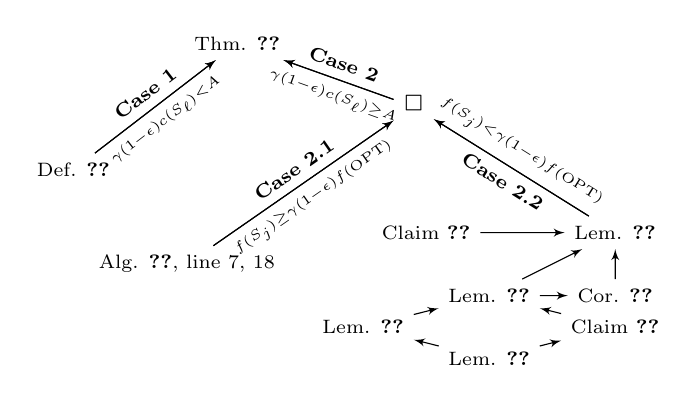
\begin{tikzpicture}[scale=0.80]
\node (1) at (0,0) {\scriptsize Thm. \ref{th:unconstrained}};
\node (2) at (-2.6,-2) {\scriptsize Def. \ref{def:weak-sub}};
\node (3) at (2.8, -1) {$\Box$};
\node (4) at (-0.8, -3.5) {\scriptsize Alg. \ref{alg:up}, line~7, 18};
\node (5) at (6, -3) {\scriptsize Lem. \ref{lem:unconstrained-h_St}};
\node (6) at (3, -3) {\scriptsize Claim \ref{claim:cost-St}};
\node (7) at (4, -4) {\scriptsize Lem. \ref{lem:h-upper-bound}};
\node (8) at (6, -4) {\scriptsize Cor. \ref{col:lower-opt}};
\node (9) at (2, -4.5) {\scriptsize Lem. \ref{lem:f-Si}};
\node (10) at (6, -4.5) {\scriptsize Claim \ref{claim:single-cost}};
\node (11) at (4, -5) {\scriptsize Lem. \ref{lem:marginal-gain}};
%edges
\draw[edge] (2) -- (1) node[midway,above,sloped] {{\bf \scriptsize Case 1}};
\draw[edge] (2) -- (1) node[midway,below,sloped] {{\bf \scriptsize $\scriptstyle \gamma(1-\epsilon)c(S_\ell) < A$}};

\draw[edge] (3) -- (1) node[midway,above,sloped] {{\bf \scriptsize Case 2}};
\draw[edge] (3) -- (1) node[midway,below,sloped] {{\bf \scriptsize $\scriptstyle\gamma(1-\epsilon)c(S_\ell) \geq A$}};

\draw[edge] (4) -- (3) node[midway,above,sloped] {{\bf \scriptsize Case 2.1}};
\draw[edge] (4) -- (3) node[midway,below,sloped] {{\bf \scriptsize $\scriptstyle f(S_j) \geq \gamma(1-\epsilon)f(\OPT)$}};

\draw[edge] (5) -- (3) node (12) [midway,below,sloped]  {{\bf \scriptsize Case 2.2}};
\draw[edge] (5) -- (3) node (12) [midway,above,sloped]  {{\bf \scriptsize $\scriptstyle f(S_j) < \gamma(1-\epsilon)f(\OPT)$}};

\draw[edge] (6) -- (5);
\draw[edge] (7) -- (5);
\draw[edge] (8) -- (5);
\draw[edge] (7) -- (8);
\draw[edge] (9) -- (7);
\draw[edge] (10) -- (7);
\draw[edge] (11) -- (9);
\draw[edge] (11) -- (10);
\end{tikzpicture}
\end{center}
\caption{Roadmap of the proof of Theorem \ref{th:unconstrained}.}
\label{fig:roadmap}
\end{figure}

\subsubsection{Useful Lemmas}
We start with Lemmas~\ref{lem:marginal-gain} and \ref{lem:f-Si}. Let $\ell$ be the value of $i$ at the termination of Algorithm \ref{alg:up}. Lemma \ref{lem:marginal-gain} lower bounds the marginal gain when adding an element to the solution set. With Lemma \ref{lem:marginal-gain}, Lemma \ref{lem:f-Si} gives the lower bound of the $f$ value of a solution set at some iteration.

\begin{lemma}
\label{lem:marginal-gain}
For all $i \in [1,\ell]$ and if $v_i$ is the element added to $S_{i-1}$, then
\[ 
f(v_i|S_{i-1}) \geq \gamma(1-\epsilon) \frac{c(v_i)}{c(\OPT)} \big ( f(\OPT) - f(S_{i-1}) \big ). 
\]
\end{lemma}

\begin{proof} 
Since $v_i$ is the element added to $S_{i-1}$ at line~14 of the algorithm,
$\frac{f(v_i|S_{i-1})}{c(v_i)}\geq {(1-\epsilon)\tau_i}$ is satisfied. Furthermore, for every 
$\forall u\in \OPT \setminus S_{i-1}$, $u$ is either equal to $v_i$ or does not satisfy the condition in line~13. Hence, 
\begin{equation}
\frac{f(v_i|S_{i-1})}{c(v_i)}\geq {(1-\epsilon)\tau_i} \geq (1-\epsilon) \frac{f(u|S_{i-1})}{c(u)}.
\label{eq:i-2}
\end{equation}

We then derive the following inequality.
\begin{align*}
    & f(\OPT)-f(S_{i-1}) \leq \frac{1}{\gamma} \sum_{u\in \OPT \setminus S_{i-1}} f(u|S_{i-1}) \quad\mbox{\tt  by Def.~(\ref{def:weak-sub})} \\
    &\leq \frac{1}{\gamma} \sum_{u\in \OPT \setminus S_{i-1}} \frac{c(u)}{1-\epsilon} \cdot \frac{f(v_i|S_{i-1})}{c(v_i)}  \quad\quad\quad\mbox{\tt  due to Eq.~(\ref{eq:i-2})} \\
    &\leq \frac{1}{\gamma(1-\epsilon)} \frac{f(v_i|S_{i-1})}{c(v_i)} c(\OPT).
\end{align*}

Rearranging the last inequality concludes the proof.     
\end{proof}

\begin{lemma}
\label{lem:f-Si}
For all $i\in [1,\ell]$, if $v_i$ is the element added to $S_{i-1}$ and $f(S_{i})=f(S_{i-1} \cup \{v_i\})$, then
\begin{equation}
    \label{eq:f-Si}
    % \scriptsize
    f(S_{i}) \geq \left(   1- \prod_{s=1}^{i} \left(1- \gamma(1-\epsilon) \frac{c(v_i)}{c(\OPT)} \right)   \right) f(\OPT).
\end{equation}
\end{lemma}

{\sc Proof Sketch.}
We prove this lemma by induction. We verify the base case ($i=1$) using Lemma \ref{lem:marginal-gain}; note that
$f(\emptyset) = 0$. Next, for every $i>1$, as an induction hypothesis, assume $\forall j \in [1, i-1]$, Eq. (\ref{eq:f-Si}) holds. We can express $f(S_{j+1})$ in the form of $f(S_{j+1}) = f(S_j)+f(v_{j+1}|S_j)$, and apply Lemma ~\ref{lem:marginal-gain} to $f(v_{j+1}|S_j)$ and the induction hypothesis to $f(S_j)$ to wrap up the proof. \hfill $\Box$


\subsubsection{Proof of Theorem \ref{th:unconstrained} }

Let $S_\ell$ with size $\ell$ be the set at the termination of Algorithm \ref{alg:up}. We divide the proof of Theorem~\ref{th:unconstrained} into two cases based on the relationship between $A$ and $c(S_\ell)$. 


\textbf{Case 1}: $\gamma (1-\epsilon)c(S_\ell) < A$.
    Consider each element $u \in \OPT \setminus S_\ell$ that was not included in $S_\ell$; such an element can be categorized into two sets $O_1$ and $O_2$ with corresponding reasons.
    
     \begin{itemize}
         \item \textit{$O_1$ is the set of elements removed at line 7.\ }\\
     The density of these elements is $\leq \gamma$ at some point before the algorithm ends. Therefore, for $u \in O_1$, if $\frac{f(u|S_u)}{c(u)}$ is the density (key) of $u$ the last time it appears in the priority queue, then we have $S_u \subseteq S_\ell$. By the property of diminishing return, we have
        \begin{equation}
        \label{eq:o1}
            \frac{f(u|S_\ell)}{c(u)} \leq \frac{f(u|S_u)}{c(u)} \leq \gamma.
        \end{equation}
        \item \textit{$O_2$ is the set of elements for which the line 18 condition was not satisfied.\ }\\
    In other words, these elements have been evaluated at line 13 for $(\log \frac{n}{\gamma\epsilon})/{\epsilon}$ times. Note that for any $u \in O_2$, the initial density of $u$ in the priority queue is $\frac{f(u)}{c(u)}$. Thus, we have: 
        \begin{equation}
            \label{eq:o2}
            \frac{f(u|S_\ell)}{c(u)} \leq \frac{f(u|S_u)}{c(u)} \leq (1-\epsilon)^{\frac{\log \frac{n}{\gamma \epsilon}}{\epsilon}}  \frac{f(u)}{c(u)}.
        \end{equation}
     
    From Eq. (\ref{eq:o2}), we can further derive $\forall u \in O_2$,
    \begin{align}
    \label{eq:derive-o2}
        f(u|S_u) &\leq (1-\epsilon)^{\frac{\log \frac{n}{\gamma \epsilon}}{\epsilon}} f(u) \nonumber\\
        &\leq (1+\epsilon)^{-\frac{\log \frac{n}{\gamma \epsilon}}{\epsilon}}f(u) \quad \quad \mbox{\it due to $1-\epsilon \leq \frac{1}{1+\epsilon}$} \nonumber\\
        &\leq (1+\epsilon)^{-\frac{\log \frac{n}{\gamma \epsilon}}{\log 1+\epsilon}}f(u) \quad \quad \mbox{\it due to $\epsilon \leq \log{1+\epsilon}$}\nonumber\\
        &= (1+\epsilon)^{-\log_{1+\epsilon} \frac{n}{\gamma \epsilon}}f(u) ~~=~~\frac{\gamma \epsilon}{n} f(u).
    \end{align}
    \end{itemize}
    
    Therefore, for Case 1, we have
    \begin{align*}
        f(\OPT)-f(S_\ell)-c(\OPT) &\leq \frac{1}{\gamma}\!\!\sum_{u \in \OPT \setminus S_{\ell}}\!\!\!\!\!\! f(u|S_\ell)-c(\OPT)\\
        &\leq \frac{1}{\gamma}\left(\sum_{u \in O_1} f(u|S_\ell)+\sum_{u \in O_2} f(u|S_\ell)\right)-c(\OPT)\\
        &\leq \frac{1}{\gamma}\left(\sum_{u \in O_1} f(u|S_\ell)+\sum_{u \in O_2} f(u|S_\ell)\right)-\sum_{u \in O_1} c(u) \\
        &=\left(\sum_{u \in O_1} \frac{1}{\gamma} f(u|S_\ell) - c(u)\right)+\frac{1}{\gamma}\sum_{u \in O_2} f(u|S_\ell)\\
        &\leq 0 + \frac{1}{\gamma} \sum_{u \in O_2} \frac{\gamma \epsilon}{n} f(u) \quad \quad \mbox{\tt from  Eq. (\ref{eq:o1}) and (\ref{eq:derive-o2})}\\
        &\leq \epsilon f(\OPT) .
    \end{align*}
    The first inequality is due to monotonicity and weak-submodularity (Def.~\ref{def:weak-sub}) of $f$.  The last inequality holds because $O_2 \subseteq \OPT$, $|\OPT| \leq n$ and $f(u) \leq f(\OPT)$ for $u \in \OPT \setminus S_\ell$. Thus, we have  $f(\OPT)-f(S_\ell)-c(\OPT) \leq \frac{1}{\gamma} \sum_{u \in O_2} \frac{\gamma \epsilon}{n} f(u) \leq \epsilon f(\OPT)$. 
     
     Combining the above inequality with the Case 1 condition ($\gamma (1-\epsilon)c(S_\ell) < A$), we have 
     \begin{align*}
         f(\Tilde{S})-c(\Tilde{S})& \geq f(S_\ell)-c(S_\ell)\geq (1-\epsilon)f(\OPT)-c(\OPT)-\frac{1}{\gamma (1-\epsilon)}A.
     \end{align*}
    {This concludes the proof of the theorem for Case 1}. \hfill $\Box$


 
    \textbf{Case 2}: $\gamma (1-\epsilon)c(S_\ell) \geq A$. \\
    In this case, there exist $t\in[1, \ell]$ such that:
    \begin{equation}
        c(S_{t-1})< \frac{1}{\gamma (1-\epsilon)} A  \leq c(S_t)
        \label{eq:th1-case2}
    \end{equation}
    We further divide Case 2 into two sub-cases: (2.1) and (2.2).

\textbf{Case 2.1}: \textit{For some $j\in [1,t-1]$, $f(S_{j}) \geq \gamma (1-\epsilon)f(\OPT)$}.\\
Note that Algorithm~\ref{alg:up} outputs $\Tilde{S} = \argmax_{S_i, i \in [n]} f(S_i)-c(S_i)$.
Therefore, for some $j\in [1,t-1]$
\begin{align*}
h(\Tilde{S}) &\geq f(S_j) - c(S_j)  \geq \gamma (1-\epsilon)f(\OPT)-\frac{A}{\gamma(1-\epsilon)} \\
& \geq \gamma (1-\epsilon)f(\OPT) - c(\OPT) - \frac{A}{\gamma(1-\epsilon)} .
\end{align*}

This concludes the proof of the theorem for sub-case 2.1.  \hfill $\Box$

\textbf{Case 2.2}: \textit{For all $j \in [1,t-1]$, $f(S_{j}) < \gamma (1-\epsilon)f(\OPT)$}.\\
As illustrated in the proof path, we have already
proved the Lemmas~\ref{lem:marginal-gain} and \ref{lem:f-Si}. We will now prove the necessary properties conditioned on the sub-case 2.2. The following two claims give the properties of the cost of every single element in set $S_t$.

\begin{claim}
\label{claim:single-cost}
Under the Case 2.2, the following holds: $\forall~ j \in [1, t-1]:~ c(v_j) \leq c(\OPT)$.
\end{claim}
{\sc Proof Sketch:} We prove this claim by contradiction. Assume there exist some $j \in [1, t-1]$ that $c(v_j)>c(\OPT)$. Under Case 2.2 condition, $f(S_j) < \gamma(1-\epsilon)f(\OPT)$ is true. Then if we apply Lemma~\ref{lem:marginal-gain} to $f(v_j|S_{j-1})$ of $f(S_j)= f(S_{j-1}) + f(v_j|S_{j-1})$, we can derive $f(S_j) \geq \gamma(1-\epsilon)f(\OPT)$, which is a contradiction. \hfill $\Box$

        
\begin{claim}
\label{claim:cost-St}
Under the Case 2.2, if we denote $B_j = A-\gamma(1-\epsilon) c(S_{j})$, then we have  $c(v_t) > B_{t-1}$.
\end{claim}

\begin{proof}
\begin{align*}
    c(v_t) &= c(S_t) - c(S_{t-1}) \ \geq \frac{1}{\gamma(1-\epsilon)}A- c(S_{t-1}) \\
    &= \frac{1}{\gamma(1-\epsilon)}\big(A-\gamma (1-\epsilon)c(S_{t-1})\big) \\
       & \geq   A- \gamma (1-\epsilon)c(S_{t-1})\ = \ B_{t-1}.
\end{align*}
The first inequality follows from the case 2 condition Eq.~(\ref{eq:th1-case2}).
\end{proof}

Next, we present Lemma \ref{lem:h-upper-bound} that upper bounds the optimal objective value $f(\OPT) - c(\OPT)$. Furthermore, under the condition of Case 2.2, a corollary that upper bounds $f(S_j)$ can be derived from the lemma. As illustrated in the proof roadmap in Figure \ref{fig:roadmap}, the lemma and corollary are necessary for the proof of Lemma \ref{lem:unconstrained-h_St}, which wraps up the proof of Case 2.2 of the theorem.

\begin{lemma} 
\label{lem:h-upper-bound}
Under the Case 2.2,
% (i.e.,  there exist $t\in[1, \ell]$ such that $c(S_{t-1})< \frac{1}{\gamma (1-\epsilon)} A  \leq c(S_t)$ and for all $j\in[1, t-1]$, $f(S_{j}) < \gamma (1-\epsilon)f(\OPT)$), 
the following holds: for all $j\in [1,t-1]$, if $B_j=A-\gamma(1-\epsilon) c(S_{j})$, then
\[ 
   f(\OPT) - c(\OPT) \leq \frac{B_j(f(\OPT) - f(S_{j}))}{c(\OPT)} +f(S_{j}). 
\]
\end{lemma}

\begin{proof}
We divide this proof into two cases based on the valuations of $B_j$ and $c(\OPT)$.

\begin{itemize}
    \item If \textbf{$B_j > c(\OPT)$}: The lemma holds immediately.
    \item If \textbf{$B_j \leq c(\OPT)$}: We first solve the right hands side of the inequality by splitting it into a part with $f(S_{j})$ and without $f(S_{j})$. Then we can further apply Lemma~\ref{lem:f-Si} to the former.
\end{itemize}
\begin{align*}
    & \displaystyle\frac{B_j(f(\OPT) - f(S_{j}))}{c(\OPT)} +f(S_{j}) = \displaystyle\left(1-\frac{B_j}{c(\OPT)}\right)f(S_{j}) + \frac{B_j}{c(\OPT)}f(\OPT)\\
    &\geq  \displaystyle\left(1-\frac{B_j}{c(\OPT)}\right)\underbrace{\left(   1- \prod_{k=1}^{j}  \left(1- \gamma(1-\epsilon) \frac{c(v_k)}{c(\OPT)} \right)   \right) f(\OPT)}_{\mbox{\tt follows from Lemma~\ref{lem:f-Si}}} +\displaystyle\frac{B_j}{c(\OPT)}f(\OPT)\\
        &=f(\OPT) - \displaystyle\left(\left(1-\frac{B_j}{c(\OPT)}\right)\prod_{k=1}^{j} \left(1- \gamma(1-\epsilon) \frac{c(v_k)}{c(\OPT)} \right)\right)f(\OPT)\\
        &=\left( 1- \displaystyle\left(1-\frac{B_j}{c(\OPT)}\right)\prod_{k=1}^{j} \left(1- \gamma(1-\epsilon) \frac{c(v_k)}{c(\OPT)} \right) \right)f(\OPT)\\
        &\geq \left( 1- \displaystyle\left(1- \frac{B_j+\gamma(1-\epsilon)\cdot \sum_{k=1}^{j}c(v_k)}{(j+1)\cdot c(\OPT)} \right)^{j+1} \right)f(\OPT)
\end{align*}

The last inequality holds due to the following known inequality: 
\begin{equation}
1-\prod_{i=1}^n\left(1-\frac{x_i}{y}\right) \geq 1-\left(1-\frac{\sum_{i=1}^n x_i}{n y}\right)^n
\label{eq:prodsum}
\end{equation}
where $x_i, y \in \mathbb{R}^{+} \mbox{ and } x_i \leq y \mbox{ for } i \in [n]$.

Consider $\forall k\in [1,j], x_k = \gamma(1-\epsilon) c(v_k)$, $x_{k+1} = B_j$ and $y = c(\OPT)$. Note that, 
$\forall k\in [1,j], \gamma(1-\epsilon) c(v_k) \leq c(\OPT)$, which follows from Claim~\ref{claim:single-cost} and 
$\gamma(1-\epsilon) \leq 1$. Also, $B_j \leq c(\OPT)$ follows from the condition for this case. Therefore, the last inequality can be obtained by applying Eq.~(\ref{eq:prodsum}).

Proceeding further by using the definitions of $B_j$ and modular function $c$, the following derivations wrap up the proof.

\begin{align*}
    &\displaystyle\frac{B_j(f(\OPT) - f(S_{j}))}{c(\OPT)} +f(S_{j}) \\
    % &\geq \left( 1- \displaystyle\left(1- \frac{B_j+\gamma(1-\epsilon)\cdot \sum_{k=1}^{j}c(v_k)}{(j+1)\cdot c(\OPT)} \right)^{j+1} \right)f(\OPT)\\
    &\geq \left( 1- \displaystyle\left(1- \frac{A-\gamma(1-\epsilon)c(S_j)+\gamma(1-\epsilon) \sum_{k=1}^{j}c(v_k)}{(j+1)\cdot c(\OPT)} \right)^{j+1} \right)f(\OPT)\\
    &= \left( 1- \displaystyle\left( 1- \frac{A}{(j+1)\cdot c(\OPT)} \right)^{j+1} \right)f(\OPT) \\
        &= \left( 1- \displaystyle\left( 1- \frac{1}{j+1}\cdot \ln \frac{f(\OPT)}{c(\OPT)} \right)^{j+1} \right)f(\OPT) \\
        &\geq \left(1- e^{-\ln \displaystyle\frac{f(\OPT)}{c(\OPT)}}\right)f(\OPT) \quad \quad \mbox{\tt as $(1- \frac{c}{t} )^t \leq e^{-c}$ } \\
        &=\left( 1- \displaystyle\frac{c(\OPT)}{f(\OPT)} \right)f(\OPT)\\
        &= f(\OPT)-c(\OPT).
\end{align*}
\end{proof}
      
        
\begin{corollary} 
\label{col:lower-opt}
Under the Case 2.2,
% (i.e.,  there exist $t\in[1, \ell]$ such that $c(S_{t-1})< \frac{1}{\gamma (1-\epsilon)} A  \leq c(S_t)$ and for all $j\in[1, t-1]$, $f(S_{j}) < \gamma (1-\epsilon)f(\OPT)$), 
the following holds: 
for all $j \in  [1, t-1],$ if $B_j=A-\gamma(1-\epsilon) c(S_{j})$ then 
\[f(\OPT) -f(S_{j}) \geq \displaystyle\frac{1}{\gamma(1-\epsilon)}c(\OPT).\]
\end{corollary}

\begin{proof}

Note that, for the case $f(S_{j}) -c(S_{j})
            \geq \gamma (1-\epsilon)f(\OPT)-c(\OPT)-\displaystyle\frac{1}{\gamma (1-\epsilon)}A$, Theorem~\ref{th:unconstrained} holds immediately. 
   Hence, we consider the opposite case:
    \begin{align*}
    f(S_{j}) -c(S_{j}) &\leq f(\OPT)-c(\OPT)-\frac{1}{\gamma (1-\epsilon)}A\\
    % &=f(\OPT)-c(\OPT)- c(S_{j}) - \Big(\frac{1}{\gamma (1-\epsilon)}A -c(S_{j})\Big)\\
    % &=f(\OPT)-c(\OPT)- c(S_{j}) - \frac{1}{\gamma (1-\epsilon)}\Big(A -\gamma (1-\epsilon)c(S_{j})\Big)\\
    &=f(\OPT)-c(\OPT)- c(S_{j}) - \frac{1}{\gamma (1-\epsilon)}B_j\\
    &\leq \displaystyle\frac{B_j(f(\OPT) - f(S_{j}))}{c(\OPT)} +f(S_{j}) - c(S_{j}) - \frac{1}{\gamma (1-\epsilon)}B_j .
    \end{align*}
  
    The last inequality is due to Lemma~\ref{lem:h-upper-bound}. 
                % The above inequality implies:
                % \[ \frac{B_j(f(\OPT) - f(S_{j}))}{c(\OPT)} \geq \frac{1}{\gamma (1-\epsilon)}B_j \]
                Rearranging the above inequality concludes the proof of the corollary.
                % \[f(\OPT) -f(S_{j}) \geq \frac{1}{\gamma(1-\epsilon)}c(\OPT)\]
\end{proof}


The following lemma discharges the proof for Theorem~\ref{th:unconstrained} for the sub-case 2.2. 

\begin{lemma} 
    \label{lem:unconstrained-h_St}
Under the case 2.2,
% (i.e.,  there exist $t\in[1, \ell]$ such that $c(S_{t-1})< \frac{1}{\gamma (1-\epsilon)} A  \leq c(S_t)$ and for all $j\in[1, t-1]$, $f(S_{j}) < \gamma (1-\epsilon)f(\OPT)$),
the following holds:
    \[
    f(S_t)-c(S_t) \geq \gamma(1-\epsilon)f(\OPT)-c(\OPT) - \frac{1}{\gamma(1-\epsilon)}A
    \]
\end{lemma}

\begin{proof}
Consider $v_t$ the element added to $S_{t-1}$.
\begin{align*}
    & f(S_t)-c(S_t) =f(v_t|S_{t-1})+f(S_{t-1})-{c(S_t)}\\
    &\geq \gamma(1-\epsilon) \displaystyle\frac{c(v_t)}{c(\OPT)} \big ( f(\OPT) \!-\! f(S_{t-1}) \big ) +f(S_{t-1})\!-\!c(S_t)\\
    % & = \gamma(1-\epsilon) \displaystyle\frac{c(v_t)}{c(\OPT)} \big ( f(\OPT) - f(S_{t-1}) \big )\\
    % & \quad\quad\quad +f(S_{t-1})- {\big(c(S_{t-1})+c(v_t)\big)}\\  
    &= { \gamma(1-\epsilon) \displaystyle\frac{B_{t-1}+c(v_t)-B_{t-1}}{c(\OPT)} \big ( f(\OPT) - f(S_{t-1}) \big )}  +f(S_{t-1})- {\left(\frac{1}{\gamma(1-\epsilon)}(A-B_{t-1})+c(v_t)\right)}. 
\end{align*}
The first inequality holds from Lemma \ref{lem:marginal-gain}. The equality follows from the definition of  $B_{t-1} = A-\gamma (1-\epsilon) c(S_{t-1})$.

Proceeding further from the above inequality, 
\[
\begin{array}{rl}
& f(S_t)-c(S_t) \\
                &\geq  {\gamma(1-\epsilon) \displaystyle\frac{B_{t-1}}{c(\OPT)} \left( f(\OPT) - f(S_{t-1})\right)}+ f(S_{t-1})  \\
                &\hfill  + {\gamma(1-\epsilon) \displaystyle\frac{c(v_t)-B_{t-1}}{c(\OPT)} \left( f(\OPT) - f(S_{t-1}) \right) }\\
                 
                & \hfill- \displaystyle\frac{1}{\gamma(1-\epsilon)}A-\left(c(v_t)-\frac{1}{\gamma(1-\epsilon)}B_{t-1}\right)\\
                 
                &\geq  \gamma(1-\epsilon)  \underbrace{\left[\displaystyle\frac{B_{t-1}}{c(\OPT)} \left( f(\OPT) - f(S_{t-1}) \right) + f(S_{t-1})\right]}_{\mbox{\tt apply Lemma~\ref{lem:h-upper-bound}}}   \\
                 
                &\hfill + \gamma(1-\epsilon) \displaystyle\frac{c(v_t)-B_{t-1}}{c(\OPT)} \left( f(\OPT) - f(S_{t-1}) \right) \\
                    &\hfill- {\displaystyle\frac{1}{\gamma(1-\epsilon)}A-\big(c(v_t)-B_{t-1}\big)}\\   
                &\geq \gamma(1-\epsilon) (f(\OPT)-c(\OPT)) - \displaystyle\frac{1}{\gamma(1-\epsilon)}A \\
                &\hfill + \underbrace{\left[c(v_t)-B_{t-1}\right]\left( \gamma(1-\epsilon) \displaystyle\frac{f(\OPT) - f(S_{t-1})}{c(\OPT)} -1 \right)}_{\mbox{\tt residual value }}. 
\end{array}
\]

Note that, in Claim \ref{claim:cost-St}, we have established $c(v_t)\geq B_{t-1}$. Furthermore, from Corollary \ref{col:lower-opt}, we know
$f(\OPT) - f(S_j) \geq \frac{1}{\gamma(1-\epsilon)}{c(\OPT)}$. Therefore, 
% \[
% (c(v_t)-B_{t-1})\left( \gamma(1-\epsilon) \frac{f(\OPT) - f(S_{t-1})}{c(\OPT)} -1 \right)
% \]
the residual value is non-negative. Hence, 
\begin{align*}
   &f(\Tilde{S})-c(\Tilde{S}) \geq f(S_t)-c(S_t)\geq \gamma(1-\epsilon)f(\OPT)-c(\OPT)-\frac{1}{\gamma (1-\epsilon)}A.
\end{align*}
\end{proof}
This concludes the proof of Theorem~\ref{th:unconstrained} for case 2.2. We have proved the approximation guarantee of Theorem \ref{th:unconstrained} for every case. The following lemma finishes the proof of Theorem \ref{th:unconstrained} by bounding the worst-case running time of Algorithm \ref{alg:up}. 

\begin{lemma}
    \label{lem:time}
    The time complexity of Algorithm \ref{alg:up} is 
    %$\Tilde{\mathcal{O}}(\frac{n}{\epsilon})$ or 
    $\mathcal{O}(\frac{n}{\epsilon} \log \frac{n}{\epsilon \gamma})$.
\end{lemma}
\begin{proof}
    As per line 18 of Algorithm \ref{alg:up}, each element $e \in V$ can be evaluated for at most $(\log \frac{n}{\gamma \epsilon})/{\epsilon}$ times. Each such consideration involves one oracle call to the function $f$. Therefore, the maximal total number of oracle calls for $n$ elements is $n \cdot (\log \frac{n}{\gamma \epsilon})/{\epsilon} \in \mathcal{O}(\frac{n}{\epsilon} \log \frac{n}{\epsilon \gamma})$. 
\end{proof}


\subsubsection{Approximation Guarantee with Approximate Oracles}
To complement our proposed efficient algorithm, we provide an approximation guarantee of Algorithm \ref{alg:up} for the RUASM problem ($f$ is $\delta$-approximate to a weakly submodular function). 

\begin{theorem}
\label{th:unconstrained-approx}
    Suppose the input utility function is $\delta$-approximate to a monotone $\gamma$-submodular set function $f$, $c$ is a modular cost function, $\epsilon \in (0,1)$ is an error threshold. Let $\OPT =  \argmax_{T \subseteq V}\{f(T)-c(T)\}$, after $\mathcal{O}(\frac{n}{\epsilon}\log \frac{n}{\gamma \epsilon})$ oracle calls to the $\delta$-approximate utility function,  Algorithm \ref{alg:up} outputs $\Tilde{S}$ such that
    \begin{align*}
        f(\Tilde{S})-c(\Tilde{S}) \geq &\gamma(1-\epsilon)f(\OPT)-c(\OPT)-\frac{1}{\gamma (1-\epsilon)}A \\
        &\quad\quad- 2\delta\left(\beta+ \frac{n}{\gamma} + 1 + n(1-\epsilon)\beta'\right)
    \end{align*}
    where $A = c(\OPT) \log \frac{f(\OPT)}{c(\OPT)}$, $\beta = \frac{c(\OPT)}{c_{\min}}$ and $\beta' = \frac{c_{max}}{c(\OPT)}$.
\end{theorem}
Theorem \ref{th:unconstrained-approx} generalizes both Theorem \ref{th:unconstrained} (with $\delta=0$) and ROI \cite{jin2021unconstrained} (with $\delta=0$ and $\epsilon=0$). 
The proof of Theorem \ref{th:unconstrained-approx} follows the roadmap as shown in Figure \ref{fig:roadmap} with moderate modifications to some lemmas. The detailed derivations are presented in the Appendix (Section \ref{sec:unconstrained-approx}).% --- end sections/3-unconstrained.tex ---
% --- begin sections/5-results.tex ---
\section{Experiments}
\label{sec:experiments} 

Our experiments are conducted on a MacBook Pro with an M1 Pro chip and 16GB RAM, and all algorithms are implemented in C++ \footnote{The code can be found: \url{https://github.com/yz24/UWSM}.}.
We have implemented lazy evaluations \cite{minoux2005accelerated} for algorithms with submodular function $f$, for example, ROI and our UP. 
We discuss the applications of profit maximization, vertex cover with costs, and Bayesian A-Optimal design. The latter is specifically for weakly submodular $f$ functions.

\subsection{Baseline Algorithms} 
We compare our algorithm \textsc{UP} with the modified \textsc{ROI}  and \textsc{UDG}~\cite{harshaw2019submodular}. 

\paragraph{\bf Modified ROI} Note that ROI greedy as presented in \cite{jin2021unconstrained} does not provide approximation guarantees when the function $f$ is weakly submodular.
We have developed a modified version of the ROI greedy algorithm to accommodate for weakly submodular $f$. The algorithm runs at most $n$ iterations and during each iteration, it adds an element with the maximal density w.r.t. the current partial solution as long as the density is greater than $\gamma$. The output is the maximal objective value of every partial solution (same as Algorithm \ref{alg:up}). Additionally, We have established an approximation bound of the modified algorithm in Theorem \ref{th:modified-roi}.
\begin{theorem}
\label{th:modified-roi}
    Given a monotone $\gamma$-submodular function $f:2^{V} \rightarrow \mathbb{R}^{\geq 0}$ and a modular cost function $c$, with $\mathcal{O}(n^2)$ oracle calls to $f$, the modified ROI algorithm outputs $\Tilde{S}$ such that
    \[f(\Tilde{S})-c(\Tilde{S}) \geq \gamma f(\OPT)-c(\OPT)- \frac{c(\OPT)}{\gamma} \log \frac{f(\OPT)}{c(\OPT)}.\]
\end{theorem}
We notice that when the function $f$ is submodular ($\gamma=1$), the approximation reduces to the approximation result of ROI \cite{jin2021unconstrained}. 
The pseudo-code of the modified algorithm and theoretical analysis of Theorem \ref{th:modified-roi} are presented in the Appendix (Section \ref{sec:modified-roi}). We note that the modified algorithm still works in quadratic time. The rationale behind developing the modified ROI is to appropriately compare our results with the ROI algorithm when the function $f$ is weakly submodular. 


\paragraph{\bf UDG} 
The UDG algorithm is randomized and the claimed approximation bound holds in expectation. Thus, we run the UDG algorithm ten times and report the \textit{median} results returned. As for runtime, we also report the \textit{median} running time of the ten runs.

For a fair comparison among different methods, we evaluate the running time based on the number of oracle evaluations as discussed in Section \ref{sec:preliminaries}. 

\subsection{Applications and Experimental Settings}
In this subsection, we formulate three applications that apply to the proposed RUSM and RUWSM problems. We also provide the descriptions of the datasets we use for the experiments and critical parameter setups. The statistics of the datasets are presented in Tables \ref{tab:datasets-networks} and \ref{tab:datasets-others}.


\begin{table}[h]
    \centering
     \caption{Network Data Statistics}
    \begin{tabular}{ |l|c|c|c|c| } 
    \hline
    Application & Network & $n$ & $m$ & Type \\[0.2em]
    \hline
    \multirow{3}{*}{Profit Max.} & Gnutella-08 & 6,301 & 20,777 & Directed\\ [0.1em]
    & NetHEPT & 15,233 & 62,774 & Undirected \\ 
    \hline
    \multirow{3}{*}{Vertex Cover} & Protein & 1,706 & 6,207 & Directed\\ [0.1em]
    &  Eu-Email& 1,005 & 25,571 & Directed \\
    [0.1em]
    \hline
\end{tabular}
    \label{tab:datasets-networks}
\end{table}

\begin{table}[h]
    \centering
     \caption{Bayesian A-Optimal Design Data Statistics ($d$: number of attributes; $n$: number of measurements)}
    \begin{tabular}{ |l|c|c| } 
    \hline
    Dataset & $n$ & $d$  \\[0.2em]
    \hline
     Boston Housing & 506 & 14 \\ [0.1em]
     Segment & 2,310 & 19  \\ 
    [0.1em]
    \hline
\end{tabular}
    \label{tab:datasets-others}
\end{table}


\paragraph{\bf Profit Maximization.} The diffusion model \cite{kempe2003maximizing} is defined using a graph $G=(V,E)$ and a probability function $p(u,v), \forall (u,v)\in E$.   
A monotone submodular function $f(S) = \mathbb{E}[\mathrm{I}(S)]$ measures the expected number of nodes that are influenced by the set of nodes in $S$ based on a diffusion model, such as the independent cascade (IC) model \cite{kempe2003maximizing}. 
Furthermore, it is often the case that some cost $c(v)$ is associated with each node $v \in V$.
-- this is the cost incurred for including an entity in the seed
set. For instance, a highly influential entity is likely to incur higher costs than others.
Following \cite{jin2021unconstrained, tang2018towards}, we use a linear cost function $c:2^V \rightarrow \mathbb{R}^{>0}$ which is proportional to the out-degree $d(v)$ of a node $v \in V$. Formally, for every $v \in V$:
$c(v) = \lambda_1 \cdot d(v)^{\lambda_2}$, where $\lambda_1$ and $\lambda_2$ are positive cost penalty parameters. Thus, the modular cost of a set $S \subseteq V$ is $c(S)=\sum_{v\in S}c(v)$.  Note that we define $c(v)=1$ if $d(v)=0$ to avoid undefined {\em density} of node $v$.

Therefore, the {\em profit maximization} problem finds a subset $S$ of $V$ such that 
\[\argmax_{S\subseteq V} ~\mathbb{E}[\mathrm{I}(S)]-c(S).\]

For fair comparisons, we adapt the profit maximization  framework~\cite{jin2021unconstrained}, which is based on the Random Reachable (RR) approach to speed up the computation of the expected influence value~\cite{borgs2014maximizing,TangXS14,TangSX15,NguyenTD16,HuangWBXL17}. We use the standard benchmarks p2p-Gnutella-08 network \cite{leskovec2007graph} and NetHEPT network \cite{chen2009efficient}. 
We compare our algorithm with baselines by their objective values $(f-c)$ and running time with various cost penalty choices $\lambda_1$ and $\lambda_2$.

% %%%%%%%%%%%%%%%%%%%%%%%%%%%%%%%%%%%%%%%%%%%%%%%%%%%%%%

\paragraph{\bf Directed Vertex Cover with Costs. }
Let $G=(V, E)$ be a directed graph and $w: 2^V \rightarrow \mathbb{R}^{\geq 0}$ be a modular weight function on a subset of vertices. For a vertex set $S \subseteq$ $V$, let $N(S)$ denote the set of vertices which are pointed to by $S$, formally,
$N(S) \triangleq\{v \in V \mid(u, v) \in E \wedge u \in S\}$. The weighted directed vertex cover function is $f(S)=\sum_{u \in N(S) \cup S} w(u)$, which is monotone submodular. We also assume that each vertex $v \in$ $V$ has an associated non-negative cost defined by $c(v)=1+\max \{d(v)-q, 0\}$, where $d(v)$ is the out-degree of vertex $v$ and the non-negative integer $q$ is the cost penalty \cite{harshaw2019submodular}. The minimum cost of a single vertex is $1$. The larger $q$ is, the smaller the vertex costs are. 

The objective of the {\em vertex cover with costs maximization problem} is to find a subset $S$ such that 
\[\argmax_{S\subseteq V}\sum_{u \in N(S) \cup S} w(u) - \sum_{v \in S} c(v).\]
Here, function $f$ is monotone submodular, so we set $\gamma=1$. 

We use two networks in this application: Protein network \cite{stelzl2005human} and Eu-Email Core network~\cite{leskovec2007graph, yin2017local}. 
Since there is no node weight information in the datasets, for both networks, 
we assign each node a weight of 1 and a cost as defined above. For the experiments, we vary cost penalty choices $q \in [1, 12]$ and compare the objective values $(f-c)$ and running time (function calls) of our algorithm UP with ROI, UDG.


\begin{figure}[t]
\centering
\subfigure[p2p-Gnutella-08; $\lambda_2=1.2$]{
\includegraphics[width=0.22\textwidth]{figures/p2p-2.pdf}
\label{fig:p2p-1}
}
\subfigure[p2p-Gnutella-08; $\lambda_1=0.1$]{
\includegraphics[width=0.22\textwidth]{figures/p2p-1.pdf}
\label{fig:p2p-2}
}
\subfigure[NetHept; $\lambda_2=1.0$]{
\centering
\includegraphics[width=0.22\textwidth]{figures/nethept-2.pdf}
\label{fig:nethept-1}
}
\subfigure[NetHept; $\lambda_1=0.1$]{
\includegraphics[width=0.22\textwidth]{figures/nethept-1.pdf}
\label{fig:nethept-2}
% \caption{}
}
\caption{Comparisons on p2p-Gnutella31 and NetHept networks with the application of Profit Maximization.}
\end{figure}



\begin{figure}[t]
\centering
\subfigure[p2p-Gnutella31]{
\includegraphics[width=0.22\textwidth]{figures/p2p-time.pdf}
\label{fig:p2p-time}
}
\subfigure[NetHept]{
\includegraphics[width=0.22\textwidth]{figures/nethept-time.pdf}
\label{fig:nethept-time}
}
\subfigure[Vertex Cover]{
\includegraphics[width=0.22\textwidth]{figures/vertex-cover-time.pdf}
\label{fig:VC-time}
}
\subfigure[Bayesian A-Optimal Design ]{
\includegraphics[width=0.22\textwidth]{figures/bayesian-time.pdf}
\label{fig:bayesian-time}
}
\caption{Comparisons of average oracle evaluations over various cost penalties: p2p-Gnutella31 and NetHept networks (fixed $\lambda_1$ or $\lambda_2$) with Profit Maximization; various datasets with Vertex Cover and Bayesian A-Optimal Design applications. The results of UDG are one-run snap of ten runs.}
\end{figure}



\begin{figure}[t]
\centering
\subfigure[$q$ vs $f-c$; Eu-Email]{
\centering
\includegraphics[width=0.22\textwidth]{figures/email-1.pdf}
\label{fig:VC-email}
}
\subfigure[$q$ vs $f-c$; Protein]{
\includegraphics[width=0.22\textwidth]{figures/protein-1.pdf}
\label{fig:VC-protein}
}
\subfigure[$p$ vs $f-c$; Segment]{
\centering
\includegraphics[width=0.22\textwidth]{figures/segment-1.pdf}
\label{fig:bayesian-segment}
}
\subfigure[$p$ vs $f-c$; Housing]{
\includegraphics[width=0.22\textwidth]{figures/housing-1.pdf}
\label{fig:bayesian-housing}
}
\caption{Experiments with Directed Vertex Cover (Eu-Email and Protein networks) and Bayesian A-Optimal Design (Segment and Housing data).}
\end{figure}



% %%%%%%%%%%%%%%%%%%%%%%%%%%%%%%%%%%%%%%%%%%%%%%%%%%%%%%

\paragraph{\bf Bayesian A-Optimal Design. }
Given a measurement matrix $\mathbf{X}=\left[x_1, x_2, \ldots, x_n\right] \in \mathbb{R}^{d}$, a linear model $\boldsymbol{y}_S=\mathbf{X}_S^{\mathrm{T}} \boldsymbol{\theta}+$ $\zeta_S$, a modular cost function $c:2^n \rightarrow \mathbb{R}_{>0}$, where $\boldsymbol{\theta}$ has a Gaussian prior distribution $\boldsymbol{\theta} \sim$ $\mathcal{N}(0, \Sigma)$, the normal i.i.d. noise $\zeta_1, \zeta_2, \cdots, \zeta_n \sim \mathcal{N}\left(0, \sigma^2 \right)$, the objective is to find a submatrix $\mathbf{X}_S$ such that 
\[\argmax _{S \subseteq\{1,2, \ldots, n\}} f(S)-c(S).\] 
Here, 
$f(S)=\operatorname{Tr}(\Sigma)-\operatorname{Tr}\left(\Sigma^{-1}+ \frac{1}{\sigma^{2}} \mathbf{X}_S \mathbf{X}_S^{\mathrm{T}}\right)^{-1}$ is the Bayesian A-Optimality function, which is a non-negative, monotone and $\gamma$-weakly submodular function \cite{bian2017guarantees, harshaw2019submodular}. $\operatorname{Tr}(\cdot)$ denotes the trace of a matrix. 
Moreover, the marginal gain of adding a measurement $e$ to $S$ can be efficiently calculated by $f(e | S)=\frac{||z_e||^2}{\sigma^2+\left\langle x_e, z_e\right\rangle}$, where $z_e=\mathbf{M}_S^{-1} x_e$ and $\mathbf{M}_S=\Sigma^{-1}+\mathbf{X}_S \mathbf{X}_S^T$. 
The modular cost of a measurement $e \in [n]$ is defined to be proportional to its $f$ value, formally, $c(S)=\sum_{e \in S} c(e) = p\sum_{e \in S}f(e)$; $p\in (0,1)$ is the cost penalty.

We use the Boston Housing \cite{harrison1978hedonic} and Segment Data \cite{qian2021multiobjective} for this application. To prepare the datasets for analysis, we performed pre-processing tasks that involved normalizing the features to achieve a zero mean and a standard deviation of 1. In the Bayesian A-Optimality function $f(S)$, we set $\sigma=1/\sqrt{d}$.
As the submodularity ratio is not known apriori, we implemented the $\gamma$-\textsc{Guess} algorithm ~\cite{harshaw2019submodular} to \emph{estimate} an approximate $\gamma$. 
The algorithm executes Algorithm $\textsc{UP}$ or UDG for a total of $T=\lceil \frac{1}{\delta}\ln \frac{1}{\delta} \rceil$ iterations. At each iteration $r$, there is a distinct submodularity ratio $\gamma_r$. The algorithm takes this $\gamma_r$ for the solution set selection in Line 4. The outputs of the $\gamma$-\textsc{Guess} algorithm is the set with the maximum objective value and the total number of function call.
We fix the decay threshold $\delta=0.2$ in $\gamma$-\textsc{Guess} and validate our algorithm with various cost penalty choices $p\in[0.1,1.0]$. 


\subsection{Results}

\paragraph{\bf Profit Maximization}: The results varying cost penalties $\lambda_1$ and $\lambda_2$ on the benchmark networks are presented in Figures~\ref{fig:p2p-1}, \ref{fig:p2p-2}, \ref{fig:nethept-1} and \ref{fig:nethept-2}. 
The plots demonstrate that our results (Alg. UP with $\epsilon=0.1,0.2$) are close to the best-approximation algorithm ROI greedy algorithm (black-circle line) and exhibit a 15\% improvement over UDG. Regarding computational efficiency comparison in Figures \ref{fig:p2p-time} and \ref{fig:nethept-time}, our algorithm with $\epsilon=0.5$ matches the efficiency of the linear-time UDG algorithm and is 6.8 times faster than ROI. 

\paragraph{\bf Directed Vertex Cover}: Figures~\ref{fig:VC-email} and \ref{fig:VC-email} show that when the cost penalty thresholds increase, the objective values ($f-c$) also increase for every algorithm. Our algorithm demonstrates near-equivalent performance to the best-approximation algorithm \textsc{ROI}. Even with a larger $\epsilon=0.5$, our algorithm outperforms \textsc{UDG} by $25\%$ for the Protein network, particularly when dealing with high-cost penalties. The running time comparisons are depicted in Figure~\ref{fig:VC-time}.
For our algorithms with larger $\epsilon$ values, the running time aligns closely with the linear-time UDG algorithm. 

\paragraph{\bf Bayesian A-Optimal Design}:  Figures~\ref{fig:bayesian-segment}, \ref{fig:bayesian-housing}, and \ref{fig:bayesian-time} demonstrate that  
the quality of the result obtained from the modified ROI is validated against other algorithms, which is also supported by the approximation guarantee in Theorem \ref{th:modified-roi}.  Still, it needs the highest number of function calls. As for the objective values, the density maximization-based algorithms (modified ROI and UP) produce higher-quality solutions than UDG. Compared to the linear-time baseline UDG, our algorithm UP with a higher error ($\epsilon=0.5$) runs comparably fast. 


% --- end sections/5-results.tex ---
% --- begin sections/6-conclusion.tex ---
\section{Conclusion}
\label{sec:conclusion}

In this paper, we proposed a fast deterministic algorithm for balancing utility and modularity with a strong provable approximation guarantee.
We have experimentally validated our algorithms on various applications, demonstrating that our algorithms run as fast as the existing linear-time algorithms while producing comparative results as the state-of-the-art. A possible extension for future work is to investigate the approximation bound and performance when the cost function $c$ is (weakly) submodular. This would provide a more general framework and improve the applicability of the algorithms to a wider range of real-world applications.
% Another direction is to design fast deterministic algorithms for constrained $f-c$ problems.
% --- end sections/6-conclusion.tex ---

\appendix
% --- begin sections/7.1-related-work.tex ---
% \section{Additional Related and Prior Work}
% \label{sec:related}
% \paragraph{Constrained Submodular Maximization. }

% The classical work of Nemhauser et al. presented a greedy algorithm with a $(1-\nicefrac{1}{e})$ for maximizing a monotone submodular function $f$ with cardinality constraint~\cite{nemhauser:MP78}. 
% This algorithm makes $O(kn)$ calls to the submodular function. Since then, several works reduced the number of calls made. 
% Currently, the best-known deterministic algorithms for this problem achieve an approximation ratio of $(1-1/e-\epsilon)$ while making $O(\frac{n}{\epsilon})$ calls~\cite{li2022submodular,Kuhnle21}.
% For knapsack constraint,  the greedy algorithm due to Sviridenko~\cite{sviridenko2004note} achieves $(1-\nicefrac{1}{e})$ approximation ratio at the cost of a high time complexity $O(n^5)$. Subsequent research has focused on improving the algorithm's runtime while accepting a slight reduction in approximation quality~\cite{badanidiyuru2014fast, ene2017nearly, feldman2020practical,yaroslavtsev2020bring, li2022submodular,zhu2024improved}. For the matroid constraint, the natural greedy algorithm archives an approximation ratio of $1/2$~\cite{nemhauser1978analysis}. The seminal work of Calinescu et al.~\cite{calinescu2011maximizing} developed a randomized algorithm that achieves the optimal approximation ratio of $1-\nicefrac{1}{e}$. Furthermore, the work in~\cite{buchbinder2019deterministic} proposed the first deterministic algorithm with an approximation ratio of $0.5008$.   

% \paragraph{Regularize Submodular Maximization. }
% % The works in~\cite{harshaw2019submodular,nikolakaki2021efficient} studied the RUWSM problem under cardinality constraint.
% In~\cite{iyer2013submodular,PZBP23}, the authors studied the problem of maximizing $f-c$ when both $f$ and $c$ are submodular functions; on the other hand, \cite{bai2016algorithms} considered maximizing the ratio of two submodular functions. 
% Recently, it has been demonstrated that the maximization of $f-c$ and $f/c$ are equivalent~\cite{perrault2021approximation}. In \cite{zhu2013influence, lu2012profit}, the authors studied the RUSM problem in the context of information diffusion and proposed a natural greedy algorithm that maximizes the difference between marginal gain and cost. Though the algorithm is intuitive,  it does not give a theoretical bound on the solutions' quality. \citet{buchbinder2015tight} proposed a ``double greedy'' strategy for RUSM problem (where the function $f$ is submodular).   They established that the double greedy algorithm achieves an approximation ratio of $1/3$.  The algorithm presented in ~\cite{buchbinder2015tight} produces a set $S$ such that $f(S) - c(S) \geq \frac{1}{3}(f(\OPT)  - c(\OPT))$. This approximation is based on the condition that $f(S) > c(S)$ for every $S \subseteq V$.  In the same paper, the authors proposed a {\em randomized} algorithm with an improved approximation ratio of $1/2$. These algorithms make $O(n)$ oracle calls to the submodular function $f$.  However, these approximation bounds  holds only when the objective function is positive, i.e., $f(S)-c(S)>0$ for every $S \subseteq V$. However, for the general RUSM problem, we do not assume the positivity of objective value for any sets. An efficient framework was proposed in \cite{nikolakaki2021efficient} for the RUSM problem with a weak guarantee, i.e., $f(S) - c(S) \geq \frac{1}{2}f(\OPT)  - c(\OPT)$. The work of \cite{KMFK21} designed an algorithm for RUSM in steaming and MapReduce models, while \cite{LYG21} proposed a continuous greedy algorithm for the RUSM problem under a matroid constraint. 

% % The literature on submodular optimization is vast, and the articles~\cite{KG14,BF18} survey a subset of the known literature.

% % \section{Related Work on Approximate Oracles}
% % \textbf{multiplicative approximate functions}. 
% \paragraph{Submodular Maximation with Approximate Oracles. }
% For the submodular/non-submodular optimization problems with approximate oracles, \cite{qian2017subset,horel2016maximization} solved the multiplicative approximate submodular maximization under a cardinality constraint. \cite{nguyen2020streaming} proposed a streaming algorithm to maximize a $k$-submodular function with approximate oracles. Later,
% \cite{zheng2021maximizing} maximize the $\delta$- multiplicative approximate $k$-submodular functions with total and individual size constraints.  \cite{ito2019submodular} considered the submodular minimization problem under approximate oracles. \cite{huang2022efficient} present strong approximation ratios for cardinality and matroid constraint problems.
% % \textbf{additive approximate functions}. 
% Under the additive approximate oracles, \cite{hassidim2017submodular} proved that there is an algorithm with an approximation ratio arbitrarily close to the optimal $1-1/e$ when the cardinality is sufficiently large. \cite{nie2023framework} adapted offline approximate submodular maximization algorithms to Multi-Armed Bandit problems.   \cite{crawford2019submodular} obtained two approximations for the problem Submodular Cost Submodular Cover (SCSC) problem with additive approximate $f$. \cite{el2020optimal} minimized the difference of two functions $H=F-G$ under multiplicative approximate oracles where $F$ is weakly submodular and $G$ is weakly supermodular. \cite{gong2023algorithms} investigate the problems of maximizing a non-negative monotone normalized submodular function minus a non-negative modular function under the multiplicative noise in three situations, i.e., the cardinality constraint, the matroid constraint and the online unconstraint. \cite{geng2022bicriteria} focus on maximizing a non-negative monotone normalized submodular function minus a linear function under multiplicative noise and the result is similar in the case of additive noise, for the cardinality constraint and the matroid constraint.

% \medskip
% In the following, we focus on works that are closely related to ours for addressing the RUWSM problem. 

% \citet{harshaw2019submodular} presented a {\em randomized} algorithm referred to as \emph{unconstrained distorted greedy} (UDG) to address the RUWSM problem. The expected approximation guarantee for the algorithm is $(1-e^{-\gamma})f(\OPT) - c(\OPT)$. The central theme of the algorithm is to add an element to the partial solution set when the \emph{distorted gain} for the element is positive, and this process is performed $n$ times where $n$ is the number of elements. The distorted marginal profit of an element $e$ at the $i$ iteration (when the partial solution set is $S_{i-1}$) is defined as 
% \[
% \left(1-\frac{\gamma}{n}\right)^{n-i-1}f(e|S_{i-1})-c(e)
% \]
% In the above, $\gamma$ is the submodularity ratio for a weakly submodular function $f$ ($\gamma = 1$ implies the function is submodular). The number of oracle calls in the UDG algorithm is $O(n)$ owing to the necessity for computing the distorted marginal gain $n$ times. 

% Subsequently, \citet{jin2021unconstrained} developed a {\em deterministic} algorithm, referred to as ROI greedy, for addressing
% the RUSM problem (when the function $f$ is submodular). The algorithm realizes produces a set $S$ such that 
% \[
% f(S)-c(S) \geq f(\OPT)-c(\OPT) - {c(\OPT)}\log \frac{f(\OPT)}{c(\OPT)}
% \]
% The authors also proved the tightness of this approximation bound. At its core, the algorithm identifies the element with
% the maximal marginal gain density with respect to a partial solution and adds the element to the partial solution only when
% the difference between the marginal gain density is greater than the cost of the element. This process iterates $n$ times, and hence the number of oracle calls is $O(n^2)$.

% --- end sections/7.1-related-work.tex ---
% --- begin sections/7.2-full-proof.tex ---
% \section{Complete Proofs for Theorem \ref{th:unconstrained} in Section \ref{sec:unconstrained}}
% \label{sec:unconstrained-full}


% \begin{manualtheorem}{\textbf{1}}
%     \label{th:unconstrained-full}
%     Given a monotone $\gamma$-submodular function $f:2^{V} \rightarrow \mathbb{R}^{\geq 0}$ and a modular cost function $c$, an error threshold $\epsilon \in (0,1)$, after $\mathcal{O}(\frac{n}{\epsilon}\log \frac{n}{\gamma \epsilon})$ oracle calls,  Algorithm \ref{alg:up} outputs $\Tilde{S}$ such that
%     \[f(\Tilde{S})-c(\Tilde{S}) \geq \gamma(1-\epsilon)f(\OPT)-c(\OPT)- \frac{1}{\gamma(1-\epsilon)}A\]
%     \textit{where $A = c(\OPT) \log \frac{f(\OPT)}{c(\OPT)}$ and $\OPT =  \argmax_{T \subseteq V}\{f(T)-c(T)\}$.}
% \end{manualtheorem}


% \subsection{Overview of the Proof of Theorem \ref{th:unconstrained}}
% We now proceed by presenting a roadmap of the proof for Theorem~\ref{th:unconstrained} by illustrating the definitions, lemmas, and claims used to discharge the proof of the theorem. As depicted in the following tree, each node corresponds to a
% theorem, lemma, claim, etc., and the incoming directed edge captures the necessity of the source node in
% the proof of the destination node. Some edges are annotated with conditions under which the
% source node leads to the destination. For instance, if the condition in Case 2.2
% holds, Lemma \ref{lem:unconstrained-h_St} is valid and implies the validity of Theorem \ref{th:unconstrained}.  
% In our proof, we will proceed with the leaf-level lemmas and claims, and work our way towards to the root of the tree. 
% Note that we have already proved Lemmas~\ref{lem:marginal-gain} and \ref{lem:f-Si}.

% \begin{center}
% \begin{tikzpicture}[scale=0.98]

% \node (1) at (0,0) {\scriptsize Thm. \ref{th:unconstrained}};
% \node (2) at (-3,-1) {\scriptsize Def. \ref{def:weak-sub}};
% \node (3) at (3, -1) {$\Box$};
% \node (4) at (-1, -3) {\scriptsize Alg. \ref{alg:up}, line~7, 18};
% \node (5) at (6, -3) {\scriptsize Lem. \ref{lem:unconstrained-h_St}};
% \node (6) at (4, -4) {\scriptsize Claim \ref{claim:cost-St}};
% \node (7) at (5, -5) {\scriptsize Lem. \ref{lem:h-upper-bound}};
% \node (8) at (7, -4) {\scriptsize Cor. \ref{col:lower-opt}};
% \node (9) at (4, -6) {\scriptsize Lem. \ref{lem:f-Si}};
% \node (10) at (6, -6) {\scriptsize Claim \ref{claim:single-cost}};
% \node (11) at (5, -7) {\scriptsize Lem. \ref{lem:marginal-gain}};
% %edges
% \draw[edge] (2) -- (1) node[midway,below,sloped] {{\bf \scriptsize Case 1}};
% \draw[edge] (2) -- (1) node[midway,above,sloped] {{\bf \scriptsize $\scriptstyle \gamma(1-\epsilon)c(S_\ell) < A$}};

% \draw[edge] (3) -- (1) node[midway,below,sloped] {{\bf \scriptsize Case 2}};
% \draw[edge] (3) -- (1) node[midway,above,sloped] {{\bf \scriptsize $\scriptstyle\gamma(1-\epsilon)c(S_\ell) \geq A$}};

% \draw[edge] (4) -- (3) node[midway,above,sloped] {{\bf \scriptsize Case 2.1}};
% \draw[edge] (4) -- (3) node[midway,below,sloped] {{\bf \scriptsize $\scriptstyle f(S_j) \geq \gamma(1-\epsilon)f(\OPT)$}};

% \draw[edge] (5) -- (3) node (12) [midway,above,sloped]  {{\bf \scriptsize Case 2.2}};
% \draw[edge] (5) -- (3) node (12) [midway,below,sloped]  {{\bf \scriptsize $\scriptstyle f(S_j) < \gamma(1-\epsilon)f(\OPT)$}};

% \draw[edge] (6) -- (5);
% \draw[edge] (7) -- (5);
% \draw[edge] (8) -- (5);
% \draw[edge] (7) -- (8);
% \draw[edge] (9) -- (7);
% \draw[edge] (10) -- (7);
% \draw[edge] (11) -- (9);
% \draw[edge] (11) -- (10);

% \end{tikzpicture}
% \end{center}


% Before we present the proof for the above theorem, we discuss two specific properties of Algorithm~\ref{alg:up}
% in the following lemmas. Let $\ell$ be the maximal size of an intermediate solution set during the runs of the algorithm.

% \begin{manuallemma}{\textbf{2}}
%     \label{lem:marginal-gain-full}
% \textit{For all $i$ such that $1 \leq i \leq \ell$ and if $v_i$ is the element added to $S_{i-1}$, then}
% \[ 
% f(v_i|S_{i-1}) \geq \gamma(1-\epsilon) \frac{c(v_i)}{c(\OPT)} \big ( f(\OPT) - f(S_{i-1}) \big ) 
% \]
% \end{manuallemma}


% \begin{proof} 
% Given that $v_i$ is the element added to $S_{i-1}$ at line~14 of the Algorithm~\ref{alg:up}. We have
% $\displaystyle\frac{f(v_i|S_{i-1})}{c(v_i)}\geq {(1-\epsilon)\tau_i}$ due to line~13 condition. Furthermore, 
% $\forall u\in \OPT \setminus S_{i-1}$, $u$ is either equal to $v_i$ or does not satisfy the condition
% in line~13. Hence, 
% \begin{equation}\tag{3}
% \frac{f(v_i|S_{i-1})}{c(v_i)}\geq {(1-\epsilon)\tau_i} \geq (1-\epsilon) \frac{f(u|S_{i-1})}{c(u)}
% \label{eq:i-2-full}
% \end{equation}

% Since $v_i$ is added to $S_{i-1}$, we have: 
% \begin{align*}
%      f(\OPT)-f(S_{i-1})  &\leq f(\OPT \cup S_{i-1})-f(S_{i-1})  \ \quad \mbox{\it as $f$ is monotone}\\
%     &\leq \frac{1}{\gamma} \sum_{u\in \OPT \setminus S_{i-1}} f(u|S_{i-1}) \ \quad\quad\quad \mbox{\it due to Definition~\ref{def:weak-sub} (weak submodularity)} \\
%     &\leq \frac{1}{\gamma} \sum_{u\in \OPT \setminus S_{i-1}} \frac{c(u)}{1-\epsilon} \cdot \frac{f(v_i|S_{i-1})}{c(v_i)}  \quad\quad\quad\mbox{\it  due to Eq.~(\ref{eq:i-2-full})} \\
%        &=\frac{1}{\gamma(1-\epsilon)} \frac{f(v_i|S_{i-1})}{c(v_i)} \sum_{u\in \OPT \setminus S_{i-1}} c(u)\\
%        &\leq \frac{1}{\gamma(1-\epsilon)} \frac{f(v_i|S_{i-1})}{c(v_i)} c(\OPT)
% \end{align*}


% Rearranging the last inequality concludes the proof.     
% \end{proof}


% \begin{manuallemma}{\textbf{3}}
%     \label{lem:f-Si-full}
% \textit{For all $i$ such that $1 \leq i \leq \ell$, if $v_i$ is the element added to $S_{i-1}$ and $f(S_{i})=f(S_{i-1} \cup \{v_i\})$, then}
% \[ 
% f(S_{i}) \geq \left(   1- \prod_{s=1}^{i} \left(1- \gamma(1-\epsilon) \frac{c(v_i)}{c(\OPT)} \right)   \right) f(\OPT)
% \]
% \end{manuallemma}


% \begin{proof} 
% We prove this lemma by induction. We verify the base case $i=1$ using Lemma \ref{lem:marginal-gain}; note that
% $f(\emptyset) = 0$.

% Next, we prove that $f(S_i)$ holds for $i>1$. As an induction hypothesis, assume $\forall j \in [1, i -1]$,
% \[
%  f(S_{j}) \geq \left(   1- \prod_{s=1}^{j} \left(1- \gamma(1-\epsilon) \frac{c(v_s)}{c(\OPT)} \right) \right) f(\OPT)
% \]
% is true. We need to prove the inequality for $f(S_{j+1})$, 

%     \begin{align*}
%         f(S_{j+1}) &= f(S_j)+f(v_{j+1}|S_j)\\
%         &\geq f(S_j) + \gamma(1-\epsilon) \frac{c(v_{j+1})}{c(\OPT)} \left( f(\OPT) - f(S_j) \right) \quad\quad\quad\quad \mbox{\it due to Lemma~\ref{lem:marginal-gain}}\\
%         &= \gamma(1-\epsilon) \frac{c(v_{j+1})}{c(\OPT)}f(\OPT) + \left(1-\gamma(1-\epsilon) \frac{c(v_{j+1})}{c(\OPT)} \right) f(S_j)\\
%         &\geq \gamma(1-\epsilon) \frac{c(v_{j+1})}{c(\OPT)}f(\OPT) + \left(1-\gamma(1-\epsilon) \frac{c(v_{j+1})}{c(\OPT)} \right) \underbrace{\left(   1- \prod_{s=1}^{j} \left(1- \gamma(1-\epsilon) \frac{c(v_s)}{c(\OPT)} \right)   \right)f(\OPT)}_{\mbox{\it by induction hypothesis}} \\
%         &= f(\OPT) -\  f(\OPT)\left[\prod_{s=1}^{j} \left(1- \gamma(1-\epsilon) \frac{c(v_s)}{c(\OPT)} \right)\right]\left(1-\gamma(1-\epsilon) \frac{c(v_{j+1})}{c(\OPT)} \right)\\
%         &= \left(   1- \prod_{s=1}^{j+1} (1- \gamma(1-\epsilon) \frac{c(v_s)}{c(\OPT)} )   \right) f(\OPT)
%     \end{align*} 
% Thus, the inequality holds for all $i>1$. We proved this lemma.
% \end{proof}

% \subsection{Proof of the Theorem}
% Let $S_\ell$ with size $\ell$ be the set at the termination of Algorithm \ref{alg:up}. We divide the proof of Theorem~\ref{th:unconstrained} into two cases based on the relationship between $A$ and $c(S_\ell)$. Recall that $A=c(\OPT) \log \frac{f(\OPT)}{c(\OPT)}$. \\
%     
%     \textbf{Case 1}: $\gamma (1-\epsilon)c(S_\ell) < A$.\\
%     Consider each element $u \in \OPT \setminus S_\ell$ that was not included into $S_\ell$; such an element can be categorized into two sets $O_1$ and $O_2$ with corresponding reasons:

%      $\bullet$ \textit{$O_1$ is the set of elements for which the Line 7 condition was not satisfied.\ } \\
%      The density of these elements is $\leq \gamma$ at some point before the algorithm terminates. Therefore, for $u \in O_1$, if $\frac{f(u|S_u)}{c(u)}$ is the density (key) of $u$ the last time it appears in the priority queue, then 
%         \begin{equation}\tag{5}
%         \label{eq:o1-full}
%             \frac{f(u|S_\ell)}{c(u)} \leq \frac{f(u|S_u)}{c(u)} \leq \gamma
%         \end{equation}
        
%     $\bullet$ \textit{$O_2$ is the set of elements for which the Line 18 condition was not satisfied.\ } \\
%     In other words, These elements  have been considered for $\frac{\log \frac{n}{\gamma\epsilon}}{\epsilon} $ times. Note that for any $u \in O_2$, the initial density of $u$ in the priority queue is $\frac{f(u)}{c(u)}$. Then, suppose $\frac{f(u|S_u)}{c(u)}$ is the key of $u$ the last time it existed in $PQ$. Therefore, as $S_u \subseteq S_\ell$ we have 
%         \begin{equation}\tag{6}
%             \label{eq:o2-full}
%             \frac{f(u|S_\ell)}{c(u)} \leq \frac{f(u|S_u)}{c(u)} \leq (1-\epsilon)^{\frac{\log \frac{n}{\gamma \epsilon}}{\epsilon}}  \frac{f(u)}{c(u)}
%         \end{equation}


%     Therefore,
%     \begin{align*}
%         f(\OPT)-f(S_\ell)-c(\OPT) &\leq f(\OPT \cup S_\ell)-f(S_\ell)-c(\OPT) \quad \quad \mbox{\it due to monotonicity of $f$}\\
%         &\leq \frac{1}{\gamma}\sum_{u \in \OPT \setminus S_{\ell}} f(u|S_\ell)-c(\OPT) \quad \quad \quad \mbox{\it due to Definition~\ref{def:weak-sub}}\\
%         &\leq \frac{1}{\gamma}\left(\sum_{u \in O_1} f(u|S_\ell)+\sum_{u \in O_2} f(u|S_\ell)\right)-c(\OPT)\\
%         &\leq \frac{1}{\gamma}\left(\sum_{u \in O_1} f(u|S_\ell)+\sum_{u \in O_2} f(u|S_\ell)\right)-\sum_{u \in O_1} c(u) \ \ \ \ \ \mbox{\it as $c$ is modular}\\
%         &=\left(\sum_{u \in O_1} \frac{1}{\gamma} f(u|S_\ell) - c(u)\right)+\frac{1}{\gamma}\sum_{u \in O_2} f(u|S_\ell)\\
%         &\leq 0 + \frac{1}{\gamma} \sum_{u \in O_2} f(u|S_u) \quad \quad \quad \mbox{\it from Eq. (\ref{eq:o1-full})}\\
%         &\leq \frac{1}{\gamma} \sum_{u \in O_2} (1-\epsilon)^{\frac{\log \frac{n}{\gamma \epsilon}}{\epsilon}}f(u) \quad \quad \mbox{\it from Eq. (\ref{eq:o2-full})}\\
%         &\leq \frac{1}{\gamma} \sum_{u \in O_2} (1+\epsilon)^{-\frac{\log \frac{n}{\gamma \epsilon}}{\epsilon}}f(u) \quad \quad \mbox{\it due to $1-\epsilon \leq \frac{1}{1+\epsilon}$}\\
%         &\leq \frac{1}{\gamma} \sum_{u \in O_2} (1+\epsilon)^{-\frac{\log \frac{n}{\gamma \epsilon}}{\log (1+\epsilon)}}f(u) \quad \quad \mbox{\it due to $\epsilon \leq \log (1+\epsilon)$}\\
%         &= \frac{1}{\gamma} \sum_{u \in O_2} (1+\epsilon)^{-\log_{1+\epsilon} \frac{n}{\gamma \epsilon}}f(u) \\
%         &= \frac{1}{\gamma} \sum_{u \in O_2} \frac{\gamma \epsilon}{n} f(u)\\
%         &\leq \epsilon f(\OPT) 
%     \end{align*}
%     The last inequality holds because $O_2 \subseteq \OPT$, $|\OPT| \leq n$ and $f(u) \leq f(\OPT)$.
%      Thus, rearranging the above inequality and combining it with the condition for Case 1 ($0< \frac{1}{\gamma (1-\epsilon)}A-c(S_\ell)$), we obtain
%      \[ 
%      f(\OPT)-f(S_\ell)-c(\OPT) - \epsilon f(\OPT) \leq 0 \leq \frac{1}{\gamma (1-\epsilon)}A-c(S_\ell) 
%      \]
     
%      Recall that $\Tilde{S}$ is the output with the best objective value. So, 
%      \begin{align*}
%          f(\Tilde{S})-c(\Tilde{S}) &\geq f(S_\ell)-c(S_\ell)\\
%          &\geq (1-\epsilon)f(\OPT)-c(\OPT)-\frac{1}{\gamma (1-\epsilon)}A
%      \end{align*}

%     {This concludes the proof of the theorem for case 1}. \hfill $\Box$

% \smallskip
%  
%     \textbf{Case 2}: $\gamma (1-\epsilon)c(S_\ell) \geq A$. 
    
%     In this case, there exist $t\in[1, \ell]$ such that:
%     \begin{equation}\tag{7}
%         c(S_{t-1})< \frac{1}{\gamma (1-\epsilon)} A  \leq c(S_t)
%         \label{eq:th1-case2-full}
%     \end{equation}
%     Consider $j \in [1, t-1]$, we further divide Case 2 into two sub-cases: (2.1) and (2.2), where sub-case 2.1 corresponds to $f(S_{j}) \geq \gamma (1-\epsilon)f(\OPT)$ for some $j \in [1,t-1]$,  and sub-case 2.2 corresponds to $f(S_{j}) < \gamma (1-\epsilon)f(\OPT)$ for all $j \in [1,t-1]$.

% \textbf{Case 2.1}: For some $j\in [1,t-1]$, $f(S_{j}) \geq \gamma (1-\epsilon)f(\OPT)$.

% Note that Algorithm~\ref{alg:up} outputs $\Tilde{S} = \argmax_{S_i, i \in [n]} f(S_i)-c(S_i)$.
% Therefore, 
% \[
% \begin{array}{rcll}
% f(\Tilde{S}) - c(\Tilde{S}) & >& f(S_j) - c(S_j) \\
% &  \geq & \gamma (1-\epsilon)f(\OPT) - \displaystyle\frac{A}{\gamma(1-\epsilon)} & \\
% &  & \mbox{\it follows from  condition in Case 2.1 and Eq.~(\ref{eq:th1-case2-full}) implied by case 2.} \\
% & \geq & \gamma (1-\epsilon)f(\OPT) - c(\OPT) - \displaystyle\frac{A}{\gamma(1-\epsilon)} & 
% \end{array}
% \]

% This concludes the proof of the theorem for sub-case 2.1.  \hfill $\Box$

% \smallskip
% \textbf{Case 2.2}: For all $j\in [1,t-1]$, $f(S_{j}) < \gamma (1-\epsilon)f(\OPT)$.

% As illustrated in the proof-path, we have already
% proved the Lemmas~\ref{lem:marginal-gain} and \ref{lem:f-Si}. We will now prove
% the necessary properties (Claim \ref{claim:single-cost} and \ref{claim:cost-St}) conditioned on the sub-case 2.2. 

% \medskip
% \begin{manualclaim}{4}
%     % \label{claim:single-cost}
% \textit{Under the case 2.2 (i.e., 
% there exist $t\in[1, \ell]$ such that
% $c(S_{t-1})< \frac{1}{\gamma (1-\epsilon)} A  \leq c(S_t)$
% and for all $j\in[1, t-1]$, $f(S_{j}) < \gamma (1-\epsilon)f(\OPT)$),
% the following holds: }
% \[\forall ~j \in [1, t-1]:~ 

% c(v_j) \leq c(\OPT)\]
% \end{manualclaim}



% \begin{proof}
% We prove this claim by contradiction. Assume there exist some $j \in [1, t-1]$ that $c(v_j)>c(\OPT)$. Also, recall that as per the condition in sub-case 2.2, we have
% \begin{equation}
% \label{eq:case2-2-full}
% \begin{array}{l}
% f(S_j) < \gamma(1-\epsilon)f(\OPT)  
% \Leftrightarrow \ f(\OPT) > \displaystyle\frac{1}{\gamma(1-\epsilon)} f(S_j) > f(S_j) >f(S_{j-1})\\
% \hfill \mbox{\it as both  $\gamma$  and $\epsilon$ are  $\leq 1$}
% \end{array}
% \end{equation}

%                  Therefore, 
%                 \begin{align*}
%                      f(S_j)&= f(S_{j-1}) + f(v_j|S_{j-1})\\
%                     &\geq f(S_{j-1}) + \gamma(1-\epsilon) \frac{c(v_j)}{c(\OPT)} \big ( f(\OPT) - f(S_{j-1}) \big )  \ \ \ \ \ \ \ \ \ \ \ \mbox{\it  follows from Lemma~\ref{lem:marginal-gain}} \\
%                     &= \gamma(1-\epsilon)\frac{c(v_j)}{c(\OPT)} f(\OPT) + \Big[ 1- \gamma(1-\epsilon)\frac{c(v_j)}{c(\OPT)} \Big]f(S_{j-1})\\
%                     &\geq { \gamma(1-\epsilon)\frac{c(v_j)}{c(\OPT)} f(\OPT)} + \gamma(1-\epsilon)\Big[ 1- \frac{c(v_j)}{c(\OPT)} \Big]f(S_{j-1})\\
%                     &= {\gamma(1-\epsilon) f(\OPT) + \gamma(1-\epsilon)\Big[ \frac{c(v_j)}{c(\OPT)} - 1 \Big]f(\OPT)} - \gamma(1-\epsilon)\Big[ \frac{c(v_j)}{c(\OPT)} - 1 \Big] f(S_{j-1})\\
%                     &= \gamma(1-\epsilon) f(\OPT) + \gamma(1-\epsilon)\Big[ \frac{c(v_j)}{c(\OPT)} - 1 \Big] \big( f(\OPT) - f(S_{j-1}) \big)\\
%                     &\geq \gamma(1-\epsilon) f(\OPT) \\
%                     & \ \ \ \ \ \ \ \ \ \ \ \ \mbox{\it follows from the assumption $c(v_j)>c(\OPT)$ and Eq.~(\ref{eq:case2-2-full})}
%                 \end{align*}
%                  Note that, using the assumption, we 
%                 have concluded that $f(S_j) \geq \gamma(1-\epsilon) f(\OPT)$, which contradicts the premise of the claim (see Eq.~(\ref{eq:case2-2-full})). Therefore, the assumption is incorrect, and the claim holds.
%             \end{proof}


% \begin{manualclaim}{5}

% \textit{Under the Case 2.2 (i.e., 
% there exist $t\in[1, \ell]$ such that
% $c(S_{t-1})< \frac{1}{\gamma (1-\epsilon)} A  \leq c(S_t)$
% and for all $j\in[1, t-1]$, $f(S_{j}) < \gamma (1-\epsilon)f(\OPT)$),
% the following holds: 
% for all $j \in [1, t-1]$ if $B_j=A-\gamma(1-\epsilon) c(S_{j})$ then,}
% \[c(v_t) > B_{t-1}\]
% \end{manualclaim}


% \begin{proof}

% \begin{align*}
%     c(v_t) &= c(S_t) - c(S_{t-1})\ \geq \frac{1}{\gamma(1-\epsilon)}A- c(S_{t-1}) \quad\quad\quad{\mbox{\it follows from the case 2 condition Eq.~(\ref{eq:th1-case2-full})}} \\
%     &= \frac{1}{\gamma(1-\epsilon)}\left(A-\gamma (1-\epsilon)c(S_{t-1})\right) \\
%     &\geq   A- \gamma (1-\epsilon)c(S_{t-1})\ = \ B_{t-1} \quad\quad\quad{\mbox{\it as both $\gamma$ and $\epsilon$ are $\leq$ 1}}
% \end{align*}
% \end{proof}


% \begin{manuallemma}{\textbf{6}}

% \textit{Under the case 2.2 (i.e., 
% there exist $t\in[1, \ell]$ such that
% $c(S_{t-1})< \frac{1}{\gamma (1-\epsilon)} A  \leq c(S_t)$
% and for all $j\in[1, t-1]$, $f(S_{j}) < \gamma (1-\epsilon)f(\OPT)$), the following
% holds:
% for all $j\in [1,t-1]$,
% if $B_j=A-\gamma(1-\epsilon) c(S_{j})$, then}
% \[ 
%    f(\OPT) - c(\OPT) \leq \frac{B_j(f(\OPT) - f(S_{j}))}{c(\OPT)} +f(S_{j}) 
% \]
% \end{manuallemma}


% \begin{proof}


% We divide this proof into two cases.

% $\bullet$ For \textbf{$B_j > c(\OPT)$}, the lemma holds immediately.

% \smallskip
% $\bullet$ We focus on \textbf{$B_j \leq c(\OPT)$}.

% \begin{align*}
%      \displaystyle\frac{B_j(f(\OPT) - f(S_{j}))}{c(\OPT)} +f(S_{j}) &= \displaystyle\left(1-\frac{B_j}{c(\OPT)})f(S_{j}\right) + \frac{B_j}{c(\OPT)}f(\OPT)\\
%         &\geq  \displaystyle\left(1-\frac{B_j}{c(\OPT)}\right)\underbrace{\left(   1- \prod_{k=1}^{j}  \left(1- \gamma(1-\epsilon) \frac{c(v_k)}{c(\OPT)} \right)   \right) f(\OPT)}_{\mbox{\it follows from Lemma~\ref{lem:f-Si}}}  + \displaystyle\frac{B_j}{c(\OPT)}f(\OPT)\\
%         &=f(\OPT) - \displaystyle\left(\left(1-\frac{B_j}{c(\OPT)}\right)\prod_{k=1}^{j} \left(1- \gamma(1-\epsilon) \frac{c(v_k)}{c(\OPT)} \right)\right)f(\OPT)\\
%         &=\left( 1- \displaystyle\left(1-\frac{B_j}{c(\OPT)}\right)\prod_{k=1}^{j} \left(1- \gamma(1-\epsilon) \frac{c(v_k)}{c(\OPT)} \right) \right)f(\OPT)
% \end{align*}

% We proceed with the following known inequality: for any 
% \[x_1, x_2, \cdots, x_n, y \in \mathbb{R}^{+} \mbox{ and } x_i \leq y \mbox{ for } i \leq n\]
% \begin{equation}
% 1-\prod_{i=1}^n\left(1-\frac{x_i}{y}\right) \geq 1-\left(1-\frac{\sum_{i=1}^n x_i}{n y}\right)^n
% \label{eq:prodsum}
% \end{equation}
% Consider $\forall k\in [1,j], x_k = \gamma(1-\epsilon) c(v_k)$, $x_{k+1} = B_j$ and $y = c(\OPT)$. Note that, 
% $\forall k\in [1,j], \gamma(1-\epsilon) c(v_k) \leq c(\OPT)$, which follows from Claim~\ref{claim:single-cost} and 
% $\gamma(1-\epsilon) \leq 1$. Also, $B_j \leq c(\OPT)$ follows from the condition for this case. 

% Therefore, by applying Eq.~(\ref{eq:prodsum}), we derive the following

% \begin{align*}
%     \displaystyle\frac{B_j(f(\OPT) - f(S_{j}))}{c(\OPT)} +f(S_{j}) &\geq \left( 1- \displaystyle\left(1- \frac{B_j+\gamma(1-\epsilon)\cdot \sum_{k=1}^{j}c(v_k)}{(j+1)\cdot c(\OPT)} \right)^{j+1} \right)f(\OPT)\\
%     &= \left( 1- \displaystyle\left(1- \frac{A-\gamma(1-\epsilon)c(S_j)+\gamma(1-\epsilon)\cdot \sum_{k=1}^{j}c(v_k)}{(j+1)\cdot c(\OPT)} \right)^{j+1} \right)f(\OPT)\\
%     & \ \ \ \ \ \ \ \ \ \ \ \ \ \ \ \ \ \ \ \ \ \ \ \ \ \ \ \ \mbox{\it follows from the definition of $B_j$} \\[1em]
%         &= \left( 1- \displaystyle\left( 1- \frac{A}{(j+1)\cdot c(\OPT)} \right)^{j+1} \right)f(\OPT) \quad\quad\quad\mbox{\it as $\sum_{k=1}^{j}c(v_k) = c(S_j)$}\\[1em]
%         &= \left( 1- \displaystyle\left( 1- \frac{1}{j+1}\cdot \ln \frac{f(\OPT)}{c(\OPT)} \right)^{j+1} \right)f(\OPT) \ \ \ \ \ \ \ \ \ \ \ \ \ \ \ \ \mbox{\it as $A=c(\OPT)\ln\frac{f(\OPT)}{c(\OPT)}$} \\[1em]
%         &\geq \left(1- e^{-\ln \displaystyle\frac{f(\OPT)}{c(\OPT)}}\right)f(\OPT) \quad \quad \quad \mbox{\it as $(1- \frac{c}{t} )^t \leq e^{-c}$ for any positive $t$} \\[1em]
%         &=\left( 1- \displaystyle\frac{c(\OPT)}{f(\OPT)} \right)f(\OPT)\\
%         &= f(\OPT)-c(\OPT)
% \end{align*}

 
% \end{proof}    

% \begin{manualcorollary}{\textbf{7}}
%     \textit{Under the case 2.2 (i.e., 
% there exist $t\in[1, \ell]$ such that
% $c(S_{t-1})< \frac{1}{\gamma (1-\epsilon)} A  \leq c(S_t)$
% and for all $j\in[1, t-1]$, $f(S_{j}) < \gamma (1-\epsilon)f(\OPT)$), the following holds: 
% for all $j \in  [1, t-1],$ 
% if $B_j=A-\gamma(1-\epsilon) c(S_{j})$ then }
% \[f(\OPT) -f(S_{j}) \geq \displaystyle\frac{1}{\gamma(1-\epsilon)}c(\OPT)\]
% \end{manualcorollary}
        


% \begin{proof}


%    Note that, for the case $f(S_{j}) -c(S_{j})
%             \geq \gamma (1-\epsilon)f(\OPT)-c(\OPT)-\displaystyle\frac{1}{\gamma (1-\epsilon)}A$, Theorem~\ref{th:unconstrained} holds immediately. 
%    Hence, we consider the case where $f(S_{j}) -c(S_{j})
%             <\gamma (1-\epsilon)f(\OPT)-c(\OPT)-\displaystyle\frac{1}{\gamma (1-\epsilon)}A$. 
%    \[
%         \begin{array}{rl}
%         &f(S_{j}) -c(S_{j}) 
%             <\gamma (1-\epsilon)f(\OPT)-c(\OPT)-\frac{1}{\gamma (1-\epsilon)}A\\
%                     &\leq \gamma (1-\epsilon)\big(f(\OPT)-c(\OPT)\big)-\frac{1}{\gamma (1-\epsilon)}A\\
%                     &\leq f(\OPT)-c(\OPT)-\frac{1}{\gamma (1-\epsilon)}A\\
%                     &=f(\OPT)-c(\OPT)- c(S_{j}) - \Big(\frac{1}{\gamma (1-\epsilon)}A -c(S_{j})\Big)\\
%                     &=f(\OPT)-c(\OPT)- c(S_{j}) - \frac{1}{\gamma (1-\epsilon)}\Big(A -\gamma (1-\epsilon)c(S_{j})\Big)\\
%                     &=f(\OPT)-c(\OPT)- c(S_{j}) - \frac{1}{\gamma (1-\epsilon)}B_j\\
%                     &\leq \displaystyle\frac{B_j(f(\OPT) - f(S_{j}))}{c(\OPT)} +f(S_{j}) - c(S_{j}) - \frac{1}{\gamma (1-\epsilon)}B_j \\
%                     &  
%                 \end{array}
%                 \]
%                 The last inequality is due to Lemma~\ref{lem:h-upper-bound}.
%                 The above inequality implies:
%                 \[ \frac{B_j(f(\OPT) - f(S_{j}))}{c(\OPT)} \geq \frac{1}{\gamma (1-\epsilon)}B_j \]

%                 Rearranging the term concludes the proof of the corollary.
%                 \[f(\OPT) -f(S_{j}) \geq \frac{1}{\gamma(1-\epsilon)}c(\OPT)\]
% \end{proof}


% The following lemma discharges the proof for Theorem~\ref{th:unconstrained} for the sub-case 2.2. 


% \begin{manuallemma}{\textbf{8}}
%    \textit{ Under the case 2.2 (i.e., 
% there exist $t\in[1, \ell]$ such that
% $c(S_{t-1})< \frac{1}{\gamma (1-\epsilon)} A  \leq c(S_t)$
% and for all $j\in[1, t-1]$, $f(S_{j}) < \gamma (1-\epsilon)f(\OPT)$),
% the following holds:}
%     \[f(S_t)-c(S_t) \geq \gamma(1-\epsilon)f(\OPT)-c(\OPT) - \frac{1}{\gamma(1-\epsilon)}A\]
% \end{manuallemma}


% \begin{proof}

% Consider $v_t$ the element added to $S_{t-1}$.
% \[
%             \begin{array}{rl}
%                 & f(S_t)-c(S_t) \\[1em]
%                 &=f(v_t|S_{t-1})+f(S_{t-1})-{c(S_t)}\\
%                 &\geq \gamma(1-\epsilon) \displaystyle\frac{c(v_t)}{c(\OPT)} \big ( f(\OPT) - f(S_{t-1}) \big ) +f(S_{t-1})-c(S_t)
%                 \hfill \mbox{\it due to Lemma~\ref{lem:marginal-gain}} \\[1em]
%                 & = \gamma(1-\epsilon) \displaystyle\frac{c(v_t)}{c(\OPT)} \big ( f(\OPT) - f(S_{t-1}) \big ) +f(S_{t-1})- {\big(c(S_{t-1})+c(v_t)\big)}\\    
%                 &= { \gamma(1-\epsilon) \displaystyle\frac{B_{t-1}+c(v_t)-B_{t-1}}{c(\OPT)} \big ( f(\OPT) - f(S_{t-1}) \big )}  +f(S_{t-1})- {\left(\displaystyle\frac{1}{\gamma(1-\epsilon)}(A-B_{t-1})+c(v_t)\right)}
%             \end{array}
% \]
% The last equality follows from the definition of  $B_{t-1} = A-\gamma (1-\epsilon) c(S_{t-1})$.

% \smallskip
% Proceeding further by rearranging the terms, 
% \[
% \begin{array}{rl}
%  f(S_t)-c(S_t) &\geq  {\gamma(1-\epsilon) \displaystyle\frac{B_{t-1}}{c(\OPT)} \left( f(\OPT) - f(S_{t-1})\right)}+ f(S_{t-1})  \\
%                 &\hfill  + {\gamma(1-\epsilon) \displaystyle\frac{c(v_t)-B_{t-1}}{c(\OPT)} \left( f(\OPT) - f(S_{t-1}) \right) }\\
%                 \smallskip \smallskip
%                 & \hfill- \displaystyle\frac{1}{\gamma(1-\epsilon)}A-\left(c(v_t)-\frac{1}{\gamma(1-\epsilon)}B_{t-1}\right)\\
%                 \smallskip \smallskip
%                 &\geq  \gamma(1-\epsilon)  \underbrace{\left[\displaystyle\frac{B_{t-1}}{c(\OPT)} \left( f(\OPT) - f(S_{t-1}) \right) + f(S_{t-1})\right]}_{\mbox{\it apply Lemma~\ref{lem:h-upper-bound}}}   \\
%                 \smallskip \smallskip
%                 &\hfill + \gamma(1-\epsilon) \displaystyle\frac{c(v_t)-B_{t-1}}{c(\OPT)} \left( f(\OPT) - f(S_{t-1}) \right) \\
%                     &\hfill- {\displaystyle\frac{1}{\gamma(1-\epsilon)}A-\big(c(v_t)-B_{t-1}\big)}\\  \smallskip \smallskip
%                 &\geq \gamma(1-\epsilon) (f(\OPT)-c(\OPT)) - \displaystyle\frac{1}{\gamma(1-\epsilon)}A \\
%                 &\hfill + \left[c(v_t)-B_{t-1}\right]\left( \gamma(1-\epsilon) \displaystyle\frac{f(\OPT) - f(S_{t-1})}{c(\OPT)} -1 \right) 
% \end{array}
% \]

% Note that, in Claim \ref{claim:cost-St}, we have established $c(v_t)\geq B_{t-1}$. Furthermore, from Corollary \ref{col:lower-opt}, we know
% $f(\OPT) - f(S_j) \geq \displaystyle\frac{1}{\gamma(1-\epsilon)}{c(\OPT)}$. Therefore, 
% \[
% (c(v_t)-B_{t-1})\left( \gamma(1-\epsilon) \displaystyle\frac{f(\OPT) - f(S_{t-1})}{c(\OPT)} -1 \right)
% \]
% is non-negative. Hence, 

% \begin{align*}
%    f(\Tilde{S})-c(\Tilde{S}) &\geq f(S_t)-c(S_t)\\
%    &\geq \gamma(1-\epsilon)f(\OPT)-c(\OPT)-\frac{1}{\gamma (1-\epsilon)}A
% \end{align*}

% \end{proof}

% This concludes the proof for Theorem~\ref{th:unconstrained} for Case 2.2. 

% \begin{manuallemma}{\textbf{9}}
%     \textit{The time complexity of Algorithm \ref{alg:up} is }
%     $\mathcal{O}(\frac{n}{\epsilon} \log \frac{n}{\epsilon \gamma})$.
% \end{manuallemma}


% \begin{proof}
%     As per line 18 of Algorithm \ref{alg:up}, every element can be considered for adding to the solution set for at most $\frac{\log \frac{n}{\gamma \epsilon}}{\epsilon}$ times. Each such consideration involves in one oracle call to the function $f$. Therefore, the total number of oracle calls is $\mathcal{O}(\frac{n}{\epsilon} \log \frac{n}{\epsilon \gamma})$. 
% \end{proof}


\section{Modified ROI-Greedy and Threshold Greedy Algorithms}
\label{sec:modified-algorithms}
In this section, we provide the modified algorithms and the approximation proofs that we mentioned in Section \ref{sec:unconstrained} and Section \ref{sec:experiments}.

\subsection{Modified ROI-Greedy for Weakly submdular $f$}
\label{sec:modified-roi}
As we have mentioned in Section \ref{sec:unconstrained} and Section \ref{sec:experiments}, we have modified the ROI-Greedy \cite{jin2021unconstrained} to make it handle the weakly submodular $f$ in the RUWSM problem. The pseudocode is presented in Algorithm \ref{alg:roi-weak}.

\begin{algorithm}[H]
   \caption{\textsc{$\gamma$-ROI}($f, c, \gamma$)}
   \label{alg:roi-weak}
\begin{algorithmic}[1]
   \STATE {\bfseries Input:} utility function $f$, cost function $c$, submodularity ratio $\gamma$.
   \STATE {\bfseries Output:} $\Tilde{S} = \argmax_{S_i, i \in [n]} f(S_i)-c(S_i)$.
   \vspace{.05in}
   \STATE $S_0 \gets \emptyset$
    \FOR{$i\gets 1$ to $n$}
    \STATE $v_i \gets \argmax_{u \in V \setminus S_{i-1}} \frac{f(u \mid S_{i-1})}{c(u)}$
        \IF{$f(u \mid S_{i-1}) > \gamma \cdot c(u)$}
            \STATE $S_i \gets S_{i-1} \cup \{v_i\}$  
        \ELSE
        \STATE {\sc Break}
        \ENDIF 
    \ENDFOR
\end{algorithmic}
\end{algorithm}



\subsubsection{The Algorithm}
The algorithm greedily selects an element $v_i$ with the maximal density w.r.t. the current seed set $S_{i-1}$ as a candidate element (line 5). It adds  $v_i$ to $S_{i-1}$ only if the density is larger than the submodularity ratio $\gamma$ (line 6). Finally, instead of outputting the solution set constructed at the termination of the algorithm, the algorithm outputs a solution set with the best objective value among all the intermediate solution sets. 

The algorithm will iterate at most $n$ times, and every time it takes $\mathcal{O}(n)$ oracle calls to $f$ to find the maximal density. Therefore, the worst-case runtime is bounded by $\mathcal{O}(n^2)$.

The proceeding theorem is the theoretical bound guaranteed by this algorithm. 


\begin{theorem}
\label{th:unconstrained-greedy}
    Given a monotone $\gamma$-submodular function $f:2^{V} \rightarrow \mathbb{R}^{\geq 0}$ and a modular cost function $c$, after $\mathcal{O}(n^2)$ oracle calls,  Algorithm \ref{alg:roi-weak} outputs $\Tilde{S}$ such that
    \[f(\Tilde{S})-c(\Tilde{S}) \geq \gamma f(\OPT)-c(\OPT)- \frac{1}{\gamma}A\]
    where $A = c(\OPT) \log \frac{f(\OPT)}{c(\OPT)}$ and $\OPT =  \argmax_{T \subseteq V}\{f(T)-c(T)\}$.
\end{theorem}

\subsubsection{Analysis of Theorem \ref{th:unconstrained-greedy}}
The proof of Theorem \ref{th:unconstrained-greedy} can be adapted from the proof of Theorem \ref{th:unconstrained}. Next, we show how to modify some lemmas and results to derive Theorem \ref{th:unconstrained-greedy}.


% \begin{figure}
% \begin{center}
% \begin{tikzpicture}[scale=0.9]
% \node (1) at (0,0) {\scriptsize Thm. \ref{th:unconstrained-greedy}};
% \node (2) at (-3,-1) {\scriptsize Def. \ref{def:weak-sub}};
% \node (3) at (3, -1) {$\Box$};
% \node (4) at (-2, -3) {\scriptsize Alg. \ref{alg:roi-weak}, line~5};
% \node (5) at (7, -3) {\scriptsize Lem. \ref{lem:unconstrained-h_St-g}};
% \node (6) at (5, -4) {\scriptsize Claim \ref{claim:cost-St-g}};
% \node (7) at (7, -5) {\scriptsize Lem. \ref{lem:h-upper-bound-g}};
% \node (8) at (8, -4) {\scriptsize Cor. \ref{col:lower-opt-g}};
% \node (9) at (6, -6) {\scriptsize Lem. \ref{lem:f-Si-g}};
% \node (10) at (8, -6) {\scriptsize Claim \ref{claim:single-cost-g}};
% \node (11) at (7, -7) {\scriptsize Lem. \ref{lem:marginal-gain-g}};
% %edges
% \draw[edge] (2) -- (1) node[midway,below,sloped] {{\bf \scriptsize Case 1}};
% \draw[edge] (2) -- (1) node[midway,above,sloped] {{\bf \scriptsize $\scriptstyle \gamma c(S_\ell) < A$}};
% \draw[edge] (3) -- (1) node[midway,below,sloped] {{\bf \scriptsize Case 2}};
% \draw[edge] (3) -- (1) node[midway,above,sloped] {{\bf \scriptsize $\scriptstyle\gamma c(S_\ell) \geq A$}};
% \draw[edge] (4) -- (3) node[midway,above,sloped] {{\bf \scriptsize Case 2.1}};
% \draw[edge] (4) -- (3) node[midway,below,sloped] {{\bf \scriptsize $\scriptstyle f(S_j) \geq \gamma f(\OPT)$}};
% \draw[edge] (5) -- (3) node (12) [midway,above,sloped]  {{\bf \scriptsize Case 2.2}};
% \draw[edge] (5) -- (3) node (12) [midway,below,sloped]  {{\bf \scriptsize $\scriptstyle f(S_j) < \gamma f(\OPT)$}};
% \draw[edge] (6) -- (5);
% \draw[edge] (7) -- (5);
% \draw[edge] (8) -- (5);
% \draw[edge] (7) -- (8);
% \draw[edge] (9) -- (7);
% \draw[edge] (10) -- (7);
% \draw[edge] (11) -- (9);
% \draw[edge] (11) -- (10);
% \end{tikzpicture}
% \end{center}
% \caption{Roadmap of the proof of Theorems \ref{th:unconstrained-greedy} for Algorithm \ref{alg:roi-weak}}
% \label{fig:roadmap-g}
% \end{figure}



\begin{lemma}
\label{lem:marginal-gain-g}
For all $1 \leq i \leq \ell$ and if $v_i$ be the element added to $S_{i-1}$, then
\[ 
f(v_i|S_{i-1}) \geq \gamma \frac{c(v_i)}{c(\OPT)} \big ( f(\OPT) - f(S_{i-1}) \big ) 
\]
\end{lemma}

\begin{proof} 
Given that $v_i$ is the element added to $S_{i-1}$ at line~5 of the Algorithm~\ref{alg:roi-weak}. Therefore,
$\forall u\in \OPT \setminus S_{i-1}$, $u$ was not the element selected with the maximal density w.r.t.  $f(S_{i-1})$. Hence, 
\begin{equation}
\frac{f(v_i|S_{i-1})}{c(v_i)}\geq \frac{f(u|S_{i-1})}{c(u)}
\label{eq:i-2-g}
\end{equation}

Since $v_i$ is added to $S_{i-1}$, we have: 
\begin{align*}
     f(\OPT)-f(S_{i-1}) &\leq f(\OPT \cup S_{i-1})-f(S_{i-1})\\
     &\leq \frac{1}{\gamma} \sum_{u\in \OPT \setminus S_{i-1}} f(u|S_{i-1})  \\
    &\leq \frac{1}{\gamma} \sum_{u\in \OPT \setminus S_{i-1}} c(u) \cdot \frac{f(v_i|S_{i-1})}{c(v_i)}  \quad\quad\quad\mbox{\it  due to Eq.~(\ref{eq:i-2-g})} \\
    &\leq \frac{1}{\gamma} \frac{f(v_i|S_{i-1})}{c(v_i)} c(\OPT)
\end{align*}

The first two inequalities hold from monotonicity and weak submodularity (Def. \ref{def:weak-sub}) of $f$. Rearranging the last inequality concludes the proof.  
\end{proof}


\begin{lemma}
\label{lem:f-Si-g}
For all $i\in [1,\ell]$ and if $v_i$ is the element added to $S_{i-1}$ in the $i$-th iteration then
\begin{equation}
    \label{eq:f-Si-g}
    % \scriptsize
    f(S_{i}) \geq \left(1- \prod_{s=1}^{i} \left(1- \gamma \frac{c(v_i)}{c(\OPT)} \right)   \right) f(\OPT)
\end{equation}

\end{lemma}

% \textit{Proof Sketch:} We prove this lemma by induction. We verify the base case $i=1$ using Lemma \ref{lem:marginal-gain}; note that
% $f(\emptyset) = 0$.

% Next, for every $i>1$, as an induction hypothesis, assume $\forall j \in [1, i-1]$, Eq. (\ref{eq:f-Si-g}) holds.

% We can express $f(S_{j+1})$ in the form of $f(S_{j+1}) = f(S_j)+f(v_{j+1}|S_j)$. Then we apply Lemma ~\ref{lem:marginal-gain-g} to $f(v_{j+1}|S_j)$ and the induction hypothesis to $f(S_j)$. \hfill $\Box$



Let $S_\ell$ with size $\ell$ be the set at the termination of Algorithm \ref{alg:roi-weak}. We divide the proof of Theorem~\ref{th:unconstrained-greedy} into two cases based on the relationship between $A$ and $c(S_\ell)$. 

    \textbf{Case 1}: $\gamma c(S_\ell) < A$.\\
    Consider each element $u \in \OPT \setminus S_\ell$ that was not included into $S_\ell$, we have
    \begin{equation}
    \label{eq:o1-g}
        \frac{f(u|S_\ell)}{c(u)} \leq \frac{f(u|S_u)}{c(u)} \leq \gamma
    \end{equation}
        
    Therefore, for Case 1, we have
    \begin{align*}
        f(\OPT)-f(S_\ell)-c(\OPT) &\leq \frac{1}{\gamma}\!\!\sum_{u \in \OPT \setminus S_{\ell}} f(u|S_\ell)-c(\OPT)\\
        &\leq \frac{1}{\gamma}\sum_{u \in \OPT \setminus S_{\ell}} f(u|S_\ell)-\sum_{u \in \OPT \setminus S_{\ell}} c(u) \\
        &\leq 0 \quad \quad\quad \quad \mbox{\it follows from  Eq. (\ref{eq:o1-g})}\\
        &\leq \frac{A}{\gamma}-c(S_\ell)
    \end{align*}

     
     Combining the above inequality with the Case 1 condition ($\gamma (1-\epsilon)c(S_\ell) < A$), we have 
     \begin{align*}
         f(\Tilde{S})-c(\Tilde{S})& \geq f(S_\ell)-c(S_\ell)\\
         &\geq \gamma f(\OPT)-c(\OPT)-\frac{1}{\gamma}A
     \end{align*}

    {This concludes the proof of the theorem for Case 1}. \hfill $\Box$


 
    \textbf{Case 2}: $\gamma c(S_\ell) \geq A$. \\
    The proof of this case follows from the proofs of Theorem \ref{th:unconstrained} with $\epsilon=0$.
    
%     In this case, there exist $t\in[1, \ell]$ such that:
%     \begin{equation}
%         c(S_{t-1})< \frac{1}{\gamma } A  \leq c(S_t)
%         \label{eq:th1-case2-g}
%     \end{equation}
%     We further divide Case 2 into two sub-cases: (2.1) and (2.2).

% \textbf{Case 2.1}:\textit{For some $j\in [1,t-1]$, $f(S_{j}) \geq \gamma (1-\epsilon)f(\OPT)$}.

% Note that Algorithm~\ref{alg:up} outputs $\Tilde{S} = \argmax_{S_i, i \in [n]} f(S_i)-c(S_i)$.
% Therefore, 
% \begin{align*}
% h(\Tilde{S}) \geq f(S_j) - c(S_j)  &\geq \gamma f(\OPT)-\frac{A}{\gamma} \\
% & \geq \gamma f(\OPT) - c(\OPT) - \frac{A}{\gamma} 
% \end{align*}


% This concludes the proof of the theorem for sub-case 2.1.  \hfill $\Box$

% \textbf{Case 2.2}: \textit{For all $j \in [1,t-1]$, $f(S_{j}) < \gamma f(\OPT)$}.

% As illustrated in the proof-path, we have already
% proved the Lemmas~\ref{lem:marginal-gain-g} and \ref{lem:f-Si-g}. We will now prove the necessary properties conditioned on the sub-case 2.2. 

% The following two claims give the properties of the cost of every single element in set $S_t$.

% \smallskip
% \begin{claim}
% \label{claim:single-cost-g}
% Under the Case 2.2
% \[\forall~ j \in [1, t-1]:~ c(v_j) \leq c(\OPT)\]
% \end{claim}

% \smallskip            
% \begin{claim}
% \label{claim:cost-St-g}
% Under the Case 2.2, if we denote $B_j = A-\gamma c(S_{j})$,

% the following holds: 
%  \[c(v_t) > B_{t-1}\]
% \end{claim}


% Next, we present Lemma \ref{lem:h-upper-bound-g} that upper bounds the optimal objective value $f(\OPT) - c(\OPT)$. Furthermore, under the condition of Case 2.2, a corollary that upper bounds $f(S_j)$ can be derived from the lemma. As illustrated in the proof roadmap in Figure \ref{fig:roadmap-g}, the lemma and corollary are necessary for the proof of Lemma \ref{lem:unconstrained-h_St-g}, which wraps up the proof of Case 2.2 of the theorem.

% \begin{lemma} 
% \label{lem:h-upper-bound-g}
% Under the Case 2.2,
% the following holds: for all $j\in [1,t-1]$, if $B_j=A-\gamma c(S_{j})$, then
% \[ 
%    f(\OPT) - c(\OPT) \leq \frac{B_j(f(\OPT) - f(S_{j}))}{c(\OPT)} +f(S_{j}) 
% \]
% \end{lemma}
    
        
% \begin{corollary} 
% \label{col:lower-opt-g}
% Under the Case 2.2,
% the following holds: 
% for all $j \in  [1, t-1],$ if $B_j=A-\gamma c(S_{j})$ then 
% \[f(\OPT) -f(S_{j}) \geq \displaystyle\frac{1}{\gamma}c(\OPT)\]
% \end{corollary}

% The following lemma discharges the proof for Theorem~\ref{th:unconstrained-greedy} for the sub-case 2.2. 

% \begin{lemma} 
%     \label{lem:unconstrained-h_St-g}
% Under the case 2.2,
% the following holds:
%     \[f(S_t)-c(S_t) \geq \gamma f(\OPT)-c(\OPT) - \frac{1}{\gamma}A\]
% \end{lemma}

% \begin{proof}
% Consider $v_t$ the element added to $S_{t-1}$.

% \begin{align*}
%      f(S_t)-c(S_t) &=f(v_t|S_{t-1})+f(S_{t-1})-{c(S_t)}\\
%     &\geq \gamma \displaystyle\frac{c(v_t)}{c(\OPT)} \big ( f(\OPT) - f(S_{t-1}) \big ) +f(S_{t-1})-c(S_t)\\
%     &= { \gamma \displaystyle\frac{B_{t-1}+c(v_t)-B_{t-1}}{c(\OPT)} \big ( f(\OPT) - f(S_{t-1}) \big )}  +f(S_{t-1})- {\left(\displaystyle\frac{1}{\gamma}(A-B_{t-1})+c(v_t)\right)} 
% \end{align*}

% The first inequality holds from Lemma \ref{lem:marginal-gain-g}. The equality follows from the definition of  $B_{t-1} = A-\gamma c(S_{t-1})$.

% Proceeding further from the above inequality, 
% \begin{align*}
%     &f(S_t)-c(S_t)\\
%     &\geq  {\gamma \displaystyle\frac{B_{t-1}}{c(\OPT)} \left( f(\OPT) - f(S_{t-1})\right)}+ f(S_{t-1})  \hfill  + {\gamma \displaystyle\frac{c(v_t)-B_{t-1}}{c(\OPT)} \left( f(\OPT) - f(S_{t-1}) \right) }- \displaystyle\frac{1}{\gamma}A-\left(c(v_t)-\frac{1}{\gamma}B_{t-1}\right)\\
%                 \smallskip \smallskip
%     &\geq  \gamma  \underbrace{\left[\displaystyle\frac{B_{t-1}}{c(\OPT)} \left( f(\OPT) - f(S_{t-1}) \right) + f(S_{t-1})\right]}_{\mbox{\it apply Lemma~\ref{lem:h-upper-bound-g}}}  + \gamma  \displaystyle\frac{c(v_t)-B_{t-1}}{c(\OPT)} \left( f(\OPT) - f(S_{t-1}) \right) - {\displaystyle\frac{1}{\gamma}A-\big(c(v_t)-B_{t-1}\big)}\\   
%     &\geq \gamma  (f(\OPT)-c(\OPT)) - \displaystyle\frac{1}{\gamma }A  + \underbrace{\left[c(v_t)-B_{t-1}\right]\left( \gamma  \displaystyle\frac{f(\OPT) - f(S_{t-1})}{c(\OPT)} -1 \right)}_{\mbox{\it residual value }} 
% \end{align*}

% Note that, in Claim \ref{claim:cost-St-g}, we have established $c(v_t)\geq B_{t-1}$. Furthermore, from Corollary \ref{col:lower-opt-g}, we know
% $f(\OPT) - f(S_j) \geq \frac{1}{\gamma }{c(\OPT)}$. Therefore, 

% the residual value is non-negative. Hence, 

% \begin{align*}
%    f(\Tilde{S})-c(\Tilde{S}) &\geq f(S_t)-c(S_t)\geq \gamma f(\OPT)-c(\OPT)-\frac{1}{\gamma  }A
% \end{align*}
% \end{proof}
% This concludes the proof for Theorem~\ref{th:unconstrained-greedy} for case 2.2. 





\subsection{Threshold Greedy for Weakly submodular $f$}
\label{sec:modified-thresh}
\begin{algorithm}[tb]
   \caption{\textsc{threshold-ROI}($f, c, \gamma$)}
   \label{alg:roi-threshold}
\begin{algorithmic}[1]
   \STATE {\bfseries Input:} utility function $f$, cost function $c$, submodularity ratio $\gamma$.
   \STATE {\bfseries Output:} $\Tilde{S} = \argmax_{S_i, i \in [n]} f(S_i)-c(S_i)$.
   \vspace{.05in}
   \STATE $\tau \gets \max_{u \in V}\frac{f(u)}{c(u)}$, $S_0 \gets \emptyset$, $i \gets 1$
    \WHILE{$\tau > \gamma$}
    \FOR{$e \in V \setminus S_{i-1}$}
    \IF{$\frac{f(e\mid S_{i-1})}{c(e)} \geq \tau$}
    \STATE $S_i \gets S_{i-1} \cup \{e\}$
    \STATE $i++$
    \ENDIF
    \ENDFOR
    \STATE $\tau \gets (1-\epsilon) \tau$
    \ENDWHILE
\end{algorithmic}
\end{algorithm}

We provide more justifications for the statement (``traditional threshold adaption to the ROI-greedy admits unbounded runtime") in Section \ref{sec:unconstrained}. 

Threshold technique \cite{badanidiyuru2014fast} is usually used to design faster deterministic algorithms based on a greedy algorithm for submodular optimization problems. We show that the threshold technique can be applied to the unconstrained $f-c$ problem with a provable theoretical guarantee. However, the running time is unbounded. The pseudocode is presented in Algorithm \ref{alg:roi-threshold}.

\subsubsection{The Algorithm}
The algorithm initializes $S$ to an empty set. The threshold $\tau$ is initialized to be the largest density of a singleton (line 3), and it is dynamically updated (geometrically decay). The intuition behind the algorithm is that it starts by considering only the items with the high-density value. Then, the algorithm gradually relaxes the threshold value to consider more and more items. The parameter $\epsilon$ controls the rate at which the threshold value is relaxed.

The proceeding theorem is the theoretical bound guaranteed by this algorithm. 


\begin{theorem}
\label{th:unconstrained-thresh}
    Given a monotone $\gamma$-submodular function $f:2^{V} \rightarrow \mathbb{R}^{\geq 0}$, a modular cost function $c$, an error threshold $\epsilon \in (0,1)$, after $\mathcal{O}(\frac{n}{\epsilon}\log \tau_0)$ oracle calls,  Algorithm \ref{alg:roi-weak} outputs $\Tilde{S}$ such that
    \[f(\Tilde{S})-c(\Tilde{S}) \geq \gamma(1-\epsilon) f(\OPT)-c(\OPT)- \frac{1}{\gamma(1-\epsilon)}A\]
    where $A = c(\OPT) \log \frac{f(\OPT)}{c(\OPT)}$, $\OPT =  \argmax_{T \subseteq V}\{f(T)-c(T)\}$ and $\tau_0 = \max_{u \in V}\frac{f(u)}{c(u)}$.
\end{theorem}

\textbf{\textit{Note that $\tau_0$ is unbounded since the density of an element can be exponentially large, so the running time of this Algorithm \ref{alg:roi-threshold} can be as bad as $\mathcal{O}(n^2)$ or even worse.}}



\subsubsection{Analysis of Theorem \ref{th:unconstrained-thresh}}
The proof method of the theoretical bound of Theorem \ref{th:unconstrained-thresh} is similar to the previous theorems. We first prove the lower bound of the marginal gain when adding an element to the seed set. Then, we prove the theorem by cases.

\begin{lemma}
\label{lem:marginal-gain-t}
For all $i$ such that $1 \leq i \leq \ell$ and if $v_i$ be the element added to $S_{i-1}$ then
\[ 
f(v_i|S_{i-1}) \geq \gamma(1-\epsilon) \frac{c(v_i)}{c(\OPT)} \big ( f(\OPT) - f(S_{i-1}) \big ) 
\]
\end{lemma}

\begin{proof}
    
 Let $\tau_i$ be the value of $\tau$ at some iteration. By the algorithm, we know that $v_i$ was not selected for the previous $\tau_{i-1}$ where
$\tau_{i-1} = \frac{\tau_i}{1-\epsilon}$. In other words, 
\begin{equation}
\forall ~ u\in \OPT \setminus S_{i-1}: \frac{f(u|S_{i-1})}{c(u)}\leq \frac{\tau_i}{1-\epsilon}
\label{eq:i-1-t}
\end{equation}

Since $v_i$ is added to $S_{i-1}$, we have: 
\begin{align*}
    & f(\OPT)-f(S_{i-1}) \leq \frac{1}{\gamma} \sum_{u\in \OPT \setminus S_{i-1}} f(u|S_{i-1}) \quad\mbox{\tt  by Def.~(\ref{def:weak-sub})} \\
    &\leq \frac{1}{\gamma} \sum_{u\in \OPT \setminus S_{i-1}} \frac{c(u)}{1-\epsilon} \cdot \frac{f(v_i|S_{i-1})}{c(v_i)}  \quad\quad\quad\mbox{\tt  due to Eq.~(\ref{eq:i-2})} \\
    &\leq \frac{1}{\gamma(1-\epsilon)} \frac{f(v_i|S_{i-1})}{c(v_i)} c(\OPT).
\end{align*}
       % \[ 
       % \begin{array}{lll}
       % \displaystyle\frac{f(v_i|S_{i-1})}{c(v_i)} & \geq  & \tau_i \ = \ \tau_i \cdot \displaystyle\frac{\sum_{u \in \OPT\setminus S_{i-1}}c(u)}{c(\OPT \setminus S_{i-1})} \  = \ 
       %  \displaystyle\frac{\sum_{u \in \OPT\setminus S_{i-1}} \tau_i  \cdot c(u)}{c(\OPT \setminus S_{i-1})} \quad\quad\mbox{ due to Eq.~\ref{eq:i-1-t}}\\[2em]
       % &  \geq & 
       % \displaystyle\frac{\sum_{u \in \OPT\setminus S_{i-1}}(1-\epsilon)f(u|S_{i-1})}{c(\OPT \setminus S_{i-1})} \ \geq \
       
       % \gamma(1-\epsilon)\frac{f(\OPT)-f(S_{i-1})}{c(\OPT)} \quad\quad \mbox{ due to Def.~\ref{def:weak-sub}}
       %   \end{array}
       %   \]
  
%The second inequality holds because of the Definition \ref{def:weak-sub}. We finish the proof of this lemma by rearranging the above inequality.
%\textbf{Samik: no need of this proof in the appendix any more}    
\end{proof}

% \begin{lemma}
% \label{lem:f-Si-t}
% For all $i$ such that $1 \leq i \leq \ell$ and if $v_i$ is the element added to $S_{i-1}$, then
% \[ 
% f(S_{i}) \geq \left(   1- \prod_{s=1}^{i} \left(1- \gamma(1-\epsilon) \frac{c(v_i)}{c(\OPT)} \right)   \right) f(\OPT)
% \]
% \end{lemma}


\textbf{\textit{Notice that the above lemma gives the same property as in the proof of Theorem \ref{th:unconstrained}. The remaining proofs of Theorem \ref{th:unconstrained-thresh} are the same as the corresponding proofs of Theorem \ref{th:unconstrained}.
Therefore, readers can find the rest of the proofs in the main paper. We jump right to the running time analysis.}}

% %%%%%%%%%%%%%%% duplicate proofs %%%%%%%%%%%%%%%%%%%%%%%%%
% We divide the proof of Theorem~\ref{th:unconstrained-thresh} into two cases based on the relationship between $A$ and $c(S_\ell)$. \\
%     
%     \textbf{Case 1}: $\gamma (1-\epsilon)c(S_\ell) < A$.\\
%     At the end of the algorithm, the output is $S_\ell$.
%     Let $\tau_\ell$ be the value of $\tau$ when the algorithm selects the last element $v_\ell$. In this case, we have 
%     \begin{equation}
%     \label{eq:unconstrained-case1-t}
%         \frac{f(u|S_{\ell})}{c(u)} \leq \tau_\ell=\gamma, \quad \forall u\in \OPT \setminus S_{\ell}
%     \end{equation}
%      Proceeding further, 
%     \[
%     \begin{array}{rcll}
%         f(\OPT)-f(S_\ell)-c(\OPT) & \leq  & \displaystyle\frac{1}{\gamma}\displaystyle\sum_{u\in \OPT \setminus S_{\ell}} f(u|S_\ell) - \sum_{u\in \OPT \setminus S_{\ell}}c(u) 
%         & \mbox{\it first term is due to Def.~\ref{def:weak-sub}} \\
%         & = & \displaystyle\sum_{u\in \OPT \setminus S_{\ell}} \left( \frac{1}{\gamma}f(u|S_\ell) - c(u)\right) & \\
%         & \leq & 0 & \mbox{\it due to Eq.~\ref{eq:unconstrained-case1-t}}\\
%         & < & \frac{1}{\gamma (1-\epsilon)}A-c(S_\ell) & \mbox{\it due to Case 1 condition}
%         \end{array}
%     \]

%     Rearranging the above inequality establishes \[f(\Tilde{S})-c(\Tilde{S}) \geq f(S_\ell)-c(S_\ell) \geq \gamma(1-\epsilon)f(\OPT)-c(\OPT)- \frac{1}{\gamma(1-\epsilon)}A\]

%     
%     \textbf{Case 2}: $\gamma (1-\epsilon)c(S_\ell) \geq A$. 
%     In this case, there exist $j\in[1, \ell]$ such that:
%     \[c(S_{t-1})< \frac{1}{\gamma (1-\epsilon)} A  \leq c(S_t)\]
    
%     We further divide Case 2 into two sub-cases: (2.1) and (2.2).

%     For the sub-case 2.1 $f(S_{j}) \geq \gamma (1-\epsilon)f(\OPT)$, it is trivial that Theorem~\ref{th:unconstrained-thresh} holds. 
%     This is because $f(S_\ell) - c(S_\ell) > f(S_j) - c(S_j)$ and  $-c(S_j) \geq -\frac{1}{\gamma (1-\epsilon)} A$ in this case. 
    
%     The second sub-case 2.2 corresponds to $f(S_{j}) < \gamma (1-\epsilon)f(\OPT)$. In order to prove the theorem for this case,
%     we proceed with the following claims under the conditions for Case 2.2.
    
%     For the cost of $v_j$ and $v_t$ where $t  \in[1, \ell]$ and $j \in [1, t-1]$, we have the following two claims. 
%             \begin{claim}
%                 \label{claim:single-cost-t}
%                 For $j \in [1, t-1]$, 
%                 % Appendix Claim~\ref{app:claim:single-cost}.
%                 \[c(v_j) \leq c(\OPT)\]
%             \end{claim}


%             \begin{claim}
%                 \label{claim:cost-St-t}
%                 For $j \in [1, t-1]$, if $B_j=A-\gamma(1-\epsilon) c(S_{j})$ then \[c(v_t) > B_{t-1}\]
%             \end{claim}

%             \begin{lemma}
%                 \label{lem:h-upper-bound-t}
%                 For every $j:~1\leq j \leq t-1$ such that $\gamma (1-\epsilon)c(S_j) < A$, let $B_j=A-\gamma(1-\epsilon) c(S_{j})$, then
%                 \[ f(\OPT) - c(\OPT) \leq \frac{B_j(f(\OPT) - f(S_{j}))}{c(\OPT)} +f(S_{j}) \]
%             \end{lemma}

%             The proof of the above lemma follows from the Lemma~\ref{lem:f-Si-t} and Claim~\ref{claim:single-cost-t}, and it leads to the following
%             corollary. 
        
%             \begin{corollary}
%             \label{col:lower-opt-t}
%             For every $j:~1\leq j \leq t-1$ such that $\gamma (1-\epsilon)c(S_j) < A$,
%             \[f(\OPT) -f(S_{j}) \geq \frac{1}{\gamma(1-\epsilon)}c(\OPT)\]
%             \end{corollary}

% Based on the upper bound of the optimal solution $f(\OPT)-c(\OPT)$ in Lemma~\ref{lem:h-upper-bound-t} and Corollary~\ref{col:lower-opt-t}, we can derive the following lemma,
% which discharges the proof for Theorem~\ref{th:unconstrained-thresh} for sub-case 2.2 of case 2 
% \[
% c(S_{t-1})< \frac{1}{\gamma (1-\epsilon)} A  \leq c(S_t) \mbox{ and } f(S_{j}) < \gamma (1-\epsilon)f(\OPT)
% \]
% \begin{lemma}
%     \label{lem:unconstrained-h_St-t}
%     For $t\in[1, \ell]$ such that $c(S_{t-1})< \frac{1}{\gamma (1-\epsilon)} A  \leq c(S_t)$,
%     \[f(S_t)-c(S_t) \geq \gamma(1-\epsilon)f(\OPT)-c(\OPT) - \frac{1}{\gamma(1-\epsilon)}A\]
% \end{lemma}


% Theorem \ref{th:unconstrained-thresh} holds for the Case 2.2 due to Lemma \ref{lem:unconstrained-h_St-t},
% \[ f(\Tilde{S})-c(\Tilde{S}) \geq f(S_t)-c(S_t) \geq \gamma(1-\epsilon)f(\OPT)-c(\OPT)- \frac{1}{\gamma(1-\epsilon)}A \]

% %%%%%%%%%%%%%%%%%%%%%%%%%%%%%%%%%%%%%%%%



\begin{lemma}
   \label{obs:unconstrained-time}
The time complexity of Algorithm~\ref{alg:roi-threshold} is $\mathcal{O}(\frac{n}{\epsilon}\log \frac{\tau}{\epsilon})$. 
\end{lemma}


The for-loop runs at most $n$ times for each choice of threshold $\tau$. Let $\tau_0 = \max_{e \in V}\{\frac{f(e)}{c(e)}\}$ be the initial threshold. We know that $\gamma$ is the threshold at termination of the algorithm. If $T$ is the number of runs of the while-loop, then
\[
T = 2+\log_{(1-\epsilon)^{-1}} \frac{\tau_0}{\gamma} = 2-\frac{\ln \tau_0-\ln \gamma}{\ln 1-\epsilon}
\leq 2+\epsilon^{-1} (\ln \tau_0 -\ln \gamma) \in O(\epsilon^{-1} \log \tau_0)
\]

So, the overall run time is $\mathcal{O}(\frac{n}{\epsilon}\log \tau_0)$.









% --- end sections/7.2-full-proof.tex ---
% --- begin sections/7.3-approximate.tex ---
%%%%%%%%%%%%%%%%%%%%%%%%%%%%%%%%%%%%%%%%%%%%%%%%%%%%%%%%%%%%%%%%%%%%%%%%%%%%%%%
%%%%%%%%%%%%%%%%%%%%%%%%%%%%%%%%%%%%%%%%%%%%%%%%%%%%%%%%%%%%%%%%%%%%%%%%%%%%%%%
% APPENDIX
%%%%%%%%%%%%%%%%%%%%%%%%%%%%%%%%%%%%%%%%%%%%%%%%%%%%%%%%%%%%%%%%%%%%%%%%%%%%%%%
%%%%%%%%%%%%%%%%%%%%%%%%%%%%%%%%%%%%%%%%%%%%%%%%%%%%%%%%%%%%%%%%%%%%%%%%%%%%%%%
% \newpage
% \appendix
% \onecolumn


% \newpage
% \appendix

% \begin{center}
% \Large 
% \textbf{Appendix}
% \end{center}

% \setcounter{section}{0}

% \newtheorem{manualtheoreminner}{Theorem}
% \newenvironment{manualtheorem}[1]{%
%   \renewcommand\themanualtheoreminner{#1}%
%   \manualtheoreminner
% }{\endmanualtheoreminner}

% \newtheorem{manuallemmainner}{Lemma}
% \newenvironment{manuallemma}[1]{%
%   \renewcommand\themanuallemmainner{#1}%
%   \manuallemmainner
% }{\endmanuallemmainner}

% \newtheorem{manualclaiminner}{Claim}
% \newenvironment{manualclaim}[1]{%
%   \renewcommand\themanualclaiminner{#1}%
%   \manualclaiminner
% }{\endmanualclaiminner}

% \newtheorem{manualcorollaryinner}{Corollary}
% \newenvironment{manualcorollary}[1]{%
%   \renewcommand\themanualcorollaryinner{#1}%
%   \manualcorollaryinner
% }{\endmanualcorollaryinner}

% \newtheorem{manualobservationinner}{Observation}
% \newenvironment{manualobservation}[1]{%
%   \renewcommand\themanualobservationinner{#1}%
%   \manualobservationinner
% }{\endmanualobservationinner}

\section{Complete Proofs for Theorem \ref{th:unconstrained-approx}}
\label{sec:unconstrained-approx}


% \begin{definition}[$\delta$-approximate]
% \label{def:approximate}
% $\Tilde{f}$ is $\delta$-approximate (additive form) of $f$ if for every $S \subseteq V$,
%     \[  |f(S) - \Tilde{f}(S) | \leq \delta \]
% \end{definition}
In Algorithm \ref{alg:up}, we note that the input utility function is $\Tilde{f}$, which is $\delta$-approximate to a monotone $\gamma$-submodular set function $f$. Before presenting the theorem, we remark about the marginal gain of a $\delta$-approximate function $\Tilde{f}$.

\begin{remark}
By Definition \ref{def:approximate}, we have, for every $S \subseteq V$ and $v \in V \setminus S$
    \[ f(S) - \delta \leq \Tilde{f}(S) \leq f(S) + \delta\]
    \[ f(v \mid S) - 2\delta \leq \Tilde{f}(v \mid S) \leq \Tilde{f}(v \mid S) - 2\delta \]
\end{remark}

% \begin{remark}[multiplicative form]
% $\Tilde{f}$ is $\delta$-approximate (multiplicative form) of $f$ if for every $S \subseteq V$,
%     \[  (1-\delta)f(S) \leq \Tilde{f}(S) \leq (1+\delta)f(S) \]
% \end{remark}



\begin{manualtheorem}{\textbf{3.10}}
\textit{Suppose the input utility function is $\delta$-approximate to a monotone $\gamma$-submodular set function $f$. $c$ is a modular cost function. Let $\OPT =  \argmax_{T \subseteq V}\{f(T)-c(T)\}$, after $\mathcal{O}(\frac{n}{\epsilon}\log \frac{n}{\gamma \epsilon})$ oracle calls to the $\delta$-approximate utility function,  Algorithm \ref{alg:up} outputs $\Tilde{S}$ such that}
    \begin{align*}
        f(\Tilde{S})-c(\Tilde{S}) \geq  &\gamma(1-\epsilon)f(\OPT)-c(\OPT)-\frac{1}{\gamma (1-\epsilon)}A \\
        &\quad\quad- 2\delta\left(\beta+ \frac{n}{\gamma} + 1 + n(1-\epsilon)\beta'\right)
    \end{align*}
    \textit{where $A = c(\OPT) \log \frac{f(\OPT)}{c(\OPT)}$, $\beta = \frac{c(\OPT)}{c_{\min}}, \beta' = \frac{c_{max}}{c(\OPT)}$ and  $\epsilon \in (0,1)$ is an error threshold.}
\end{manualtheorem}


% \begin{theorem}
% \label{th:unconstrained-approx}
%     Given a monotone $\gamma$-submodular function $f:2^{V} \rightarrow \mathbb{R}^{\geq 0}$ and a modular cost function $c$. Let $\OPT =  \argmax_{T \subseteq V}\{f(T)-c(T)\}$, after $\Tilde{\mathcal{O}}(\frac{n}{\epsilon})$ oracle calls to $\Tilde{f}$,  Algorithm \ref{alg:up} outputs $\Tilde{S}$ such that
%     \[f(\Tilde{S})-c(\Tilde{S}) \geq \gamma(1-\epsilon)f(\OPT)-c(\OPT)-\frac{1}{\gamma (1-\epsilon)}A - 2\delta\left(\beta+ \frac{n}{\gamma} + 1 + n(1-\epsilon)\beta'\right)\]
%     where $A = c(\OPT) \log \frac{f(\OPT)}{c(\OPT)}$,\\
%     $c_{max} = \max_{e \in V} c(e),c_{min} = \min_{e \in V} c(e)$,\\
%     $\beta = \frac{c(\OPT)}{c_{\min}}, \beta' = \frac{c_{max}}{c(\OPT)}$.
% \end{theorem}
%

\subsection{Overview of the Proof}
We now proceed by presenting a roadmap in Figure \ref{fig:roadmap-approx} of the proof for Theorem~\ref{th:unconstrained-approx} by illustrating the definitions, lemmas, and claims that are used to discharge the proof of the theorem. Denote $\xi=2\delta\left(\beta+ \frac{n}{\gamma} + 1 + n(1-\epsilon)\beta'\right)$. As depicted in the following tree, each node corresponds to a
theorem, lemma, claim, etc., and the incoming directed edge captures the necessity of the source node in
the proof of the destination node. Some of the edges are annotated with conditions under which the
source node leads to the destination. For instance, if the condition in Case 2.2
holds, Lemma \ref{lem:unconstrained-h_St-approx} is valid and implies the validity of Theorem \ref{th:unconstrained-approx}.  
In our proof, we will proceed with the leaf-level lemmas and claims and work our way towards the root of the tree. 
Wee will prove Lemmas~\ref{lem:marginal-gain-approx} and \ref{lem:f-Si-approx} first. 


% \yz{}



\begin{figure}
\begin{center}
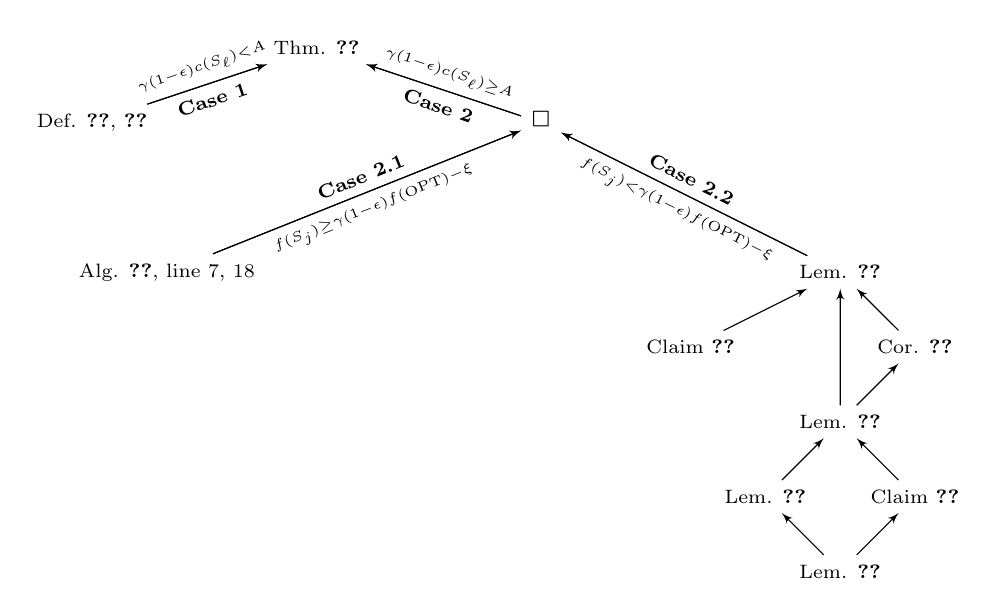
\begin{tikzpicture}[scale=0.95]

%\node[vertex] (1) at (0,0) {Theorem 1}

% vertices
\node (1) at (0,0) {\scriptsize Thm. \ref{th:unconstrained-approx}};
\node (2) at (-3,-1) {\scriptsize Def. \ref{def:weak-sub}, \ref{def:approximate}};
\node (3) at (3, -1) {$\Box$};
\node (4) at (-2, -3) {\scriptsize Alg. \ref{alg:up}, line~7, 18};
\node (5) at (7, -3) {\scriptsize Lem. \ref{lem:unconstrained-h_St-approx}};
\node (6) at (5, -4) {\scriptsize Claim \ref{claim:cost-St-approx}};
\node (7) at (7, -5) {\scriptsize Lem. \ref{lem:h-upper-bound-approx}};
\node (8) at (8, -4) {\scriptsize Cor. \ref{col:lower-opt-approx}};
\node (9) at (6, -6) {\scriptsize Lem. \ref{lem:f-Si-approx}};
\node (10) at (8, -6) {\scriptsize Claim \ref{claim:single-cost-approx}};
\node (11) at (7, -7) {\scriptsize Lem. \ref{lem:marginal-gain-approx}};
%edges
\draw[edge] (2) -- (1) node[midway,below,sloped] {{\bf \scriptsize Case 1}};
\draw[edge] (2) -- (1) node[midway,above,sloped] {{\bf \scriptsize $\scriptstyle \gamma(1-\epsilon)c(S_\ell) < A$}};

\draw[edge] (3) -- (1) node[midway,below,sloped] {{\bf \scriptsize Case 2}};
\draw[edge] (3) -- (1) node[midway,above,sloped] {{\bf \scriptsize $\scriptstyle\gamma(1-\epsilon)c(S_\ell) \geq A$}};

\draw[edge] (4) -- (3) node[midway,above,sloped] {{\bf \scriptsize Case 2.1}};
\draw[edge] (4) -- (3) node[midway,below,sloped] {{\bf \scriptsize $\scriptstyle f(S_j) \geq \gamma(1-\epsilon)f(\OPT)-\xi$}};

\draw[edge] (5) -- (3) node (12) [midway,above,sloped]  {{\bf \scriptsize Case 2.2}};
\draw[edge] (5) -- (3) node (12) [midway,below,sloped]  {{\bf \scriptsize $\scriptstyle f(S_j) < \gamma(1-\epsilon)f(\OPT)-\xi$}};

\draw[edge] (6) -- (5);
\draw[edge] (7) -- (5);
\draw[edge] (8) -- (5);
\draw[edge] (7) -- (8);
\draw[edge] (9) -- (7);
\draw[edge] (10) -- (7);
\draw[edge] (11) -- (9);
\draw[edge] (11) -- (10);
%\draw[edge, dotted,bend left] (12.225) -- (11);

%\draw[edge] (1) -- (2) node[midway, above] {$\frac{1}{3}$};
%\draw[edge] (1.260) -- (3.100);
%\draw[edge] (1.325) -- (4.125) node[pos=.3, right, sloped, rotate=90] {$\frac{1}{3}$};
%\draw[edge] (2) -- (3);
%\draw[edge] (2) -- (4) node[midway, right] {$\frac{1}{2}$};
%\draw[edge] (3.80) -- (1.280);
%\draw[edge] (4) -- (3);
%\draw[edge] (4.145) -- (1.305);
%\draw[edge] (3.170) -- (5.10);
%\draw[edge] (5.350) -- (3.190);
\end{tikzpicture}
\end{center}
\caption{Roadmap of the proof of Theorems \ref{th:unconstrained-approx} for Algorithm \ref{alg:up}}
\label{fig:roadmap-approx}
\end{figure}



\subsection{Useful Lemmas}
Before we present the proof for the above theorem, we discuss two specific properties of Algorithm~\ref{alg:up}
in the following lemmas. Let $\ell$ be the value of $i$ at the termination of Algorithm \ref{alg:up}.

\begin{lemma}
\label{lem:marginal-gain-approx}
For all $1 \leq i \leq \ell$ and if $v_i$ be the element added to $S_{i-1}$, then
\[ 
f(v_i|S_{i-1}) \geq \gamma(1-\epsilon)\frac{c(v_i)}{c(\OPT)} \left( f(\OPT)-f(S_{i-1})\right) - 2\delta  \left( 1+n\frac{(1-\epsilon)c(v_i)}{ c(\OPT)} \right) 
\]
\end{lemma}

\begin{proof} 
Since that $v_i$ is the element added to $S_{i-1}$ at line~14 of the Algorithm~\ref{alg:up}, we have
$\displaystyle\frac{\Tilde{f}(v_i|S_{i-1})}{c(v_i)}\geq {(1-\epsilon)\tau_i}$ due to line~13 condition. Furthermore, let $\displaystyle\frac{\Tilde{f}(u|S_u)}{c(u)}$ be the density when element $u$ was at the priority queue at the current iteration. Since $v_i$ is on the top of the priority queue, 
$\forall u \in \OPT \setminus S_{i-1}$, $u$ is either equal to $v_i$ or has a density $\displaystyle\frac{\Tilde{f}(u|S_u)}{c(u)}$ smaller than $\tau_i$
in Line~13. We know $S_u \subseteq S_i$. Hence, 
\begin{equation}
\frac{\Tilde{f}(v_i|S_{i-1})}{c(v_i)}\geq {(1-\epsilon)\tau_i} \geq (1-\epsilon) \frac{\Tilde{f}(u|S_{u})}{c(u)}
\label{eq:i-2-approx}
\end{equation}

By the definition of $\delta$- approximate, 
\begin{align}
    (1-\epsilon) \frac{\Tilde{f}(u|S_{u})}{c(u)} &\leq \frac{\Tilde{f}(v_i|S_{i-1})}{c(v_i)} \nonumber \\
    \Rightarrow~~  (1-\epsilon) \frac{f(u|S_{i-1})-2\delta}{c(u)} \leq (1-\epsilon) \frac{f(u|S_{u})-2\delta}{c(u)} \leq (1-\epsilon) \frac{\Tilde{f}(u|S_{u})}{c(u)} &\leq \frac{\Tilde{f}(v_i|S_{i-1})}{c(v_i)} \leq \frac{f(v_i|S_{i-1})+2\delta}{c(v_i)} \nonumber\\
    \Rightarrow~~  (1-\epsilon) \frac{f(u|S_{i-1})-2\delta}{c(u)} &\leq \frac{f(v_i|S_{i-1})+2\delta}{c(v_i)} \nonumber\\
    \Rightarrow~~  f(u|S_{i-1}) &\leq \frac{c(u)}{1-\epsilon} \cdot \frac{f(v_i|S_{i-1})+2\delta}{c(v_i)}+2\delta
    \label{eq:approx-gain-approx}
\end{align}


Since $v_i$ is added to $S_{i-1}$, we have: 
\begin{align*}
     f(\OPT)-f(S_{i-1})  &\leq f(\OPT \cup S_{i-1})-f(S_{i-1})  \ \quad\quad\quad \mbox{\it as $f$ is monotone}\\
    &\leq \frac{1}{\gamma} \sum_{u\in \OPT \setminus S_{i-1}} f(u|S_{i-1}) \ \quad\quad\quad\quad \mbox{\it due to Def.~\ref{def:weak-sub}} \\
    &\leq \frac{1}{\gamma} \sum_{u\in \OPT \setminus S_{i-1}} \left[\frac{c(u)}{1-\epsilon} \cdot \frac{f(v_i|S_{i-1})+2\delta}{c(v_i)}+2\delta \right] \quad\quad\quad\quad\mbox{\it  due to Eq. (\ref{eq:approx-gain-approx})} \\
    &=\frac{1}{\gamma(1-\epsilon)} \cdot \frac{f(v_i|S_{i-1})+2\delta}{c(v_i)} \sum_{u\in \OPT \setminus S_{i-1}} c(u) + \sum_{u\in \OPT \setminus S_{i-1}} \frac{2\delta}{\gamma}  \\
    &\leq \frac{1}{\gamma(1-\epsilon)} \cdot \frac{c(\OPT)}{c(v_i)} \Big[f(v_i|S_{i-1})+2\delta \Big]  + \frac{2n\delta}{\gamma}\\
    &= \frac{1}{\gamma(1-\epsilon)} \cdot \frac{c(\OPT)}{c(v_i)} f(v_i|S_{i-1}) + \frac{2\delta}{\gamma} \left( \frac{c(\OPT)}{(1-\epsilon)c(v_i)} + n\right)
\end{align*}

Rearranging the last inequality concludes the proof. 
\begin{align*}
    f(v_i|S_{i-1}) &\geq \gamma(1-\epsilon)\frac{c(v_i)}{c(\OPT)} \left[f(\OPT)-f(S_{i-1}) - \frac{2\delta}{\gamma} \left( \frac{c(\OPT)}{(1-\epsilon)c(v_i)} + n\right) \right]\\
    &= \gamma(1-\epsilon)\frac{c(v_i)}{c(\OPT)} \Big[ f(\OPT)-f(S_{i-1})\Big] - 2\delta  \left( 1+n\frac{(1-\epsilon)c(v_i)}{ c(\OPT)} \right) 
\end{align*}
\end{proof}

\begin{lemma}
\label{lem:f-Si-approx}
For all $i$ such that $i$ such that $1 \leq i \leq \ell$ and if $v_i$ is the element added to $S_{i-1}$ in the $i$-th iteration and $c(v_i) \leq c(\OPT)$ then
\[ 
f(S_{i}) \geq \left(   1- \prod_{s=1}^{i} \left(1- \gamma(1-\epsilon) \frac{c(v_i)}{c(\OPT)} \right)   \right) f(\OPT) - 2\delta\left(\frac{\beta}{\gamma(1-\epsilon)}+ \frac{n}{\gamma}\right)
\]
\end{lemma}

\begin{proof} 
We prove this lemma by induction. 


\textbf{Base Case: }
We verify the base case $i=1$ using Lemma \ref{lem:marginal-gain-approx}; note that
$f(\emptyset) = 0$.

\begin{align*}
    &f(S_1) = f(\{v_1\})=f(v|\emptyset) \\
    &\geq \gamma(1-\epsilon)\frac{c(v_1)}{c(\OPT)} \left[ f(\OPT)-f(S_{0})\right] - 2\delta  \left( 1+\frac{(1-\epsilon)c(v_1)}{ c(\OPT)} \right)\\
    &=\gamma(1-\epsilon)\frac{c(v_1)}{c(\OPT)}  f(\OPT) - 2\delta  \left( 1+\frac{(1-\epsilon)c(v_1)}{ c(\OPT)} \right)
\end{align*}
Since $c(v_1) \leq c(\OPT)$ and by the definition of $\beta$, $\beta = \frac{c(\OPT)}{c_{min}}$), we have:
\begin{align*}
    1+\frac{(1-\epsilon)c(v_1)}{ c(\OPT)} &\leq \frac{c(\OPT)}{c(v_1)} \left[ 1+\frac{(1-\epsilon)c(v_1)}{ c(\OPT)} \right]  \\
    &= \frac{c(\OPT)}{c(v_1)} + n(1-\epsilon) \frac{c(\OPT)}{c(v_1)}\cdot \frac{c(v_1)}{c(\OPT)}\\
    &\leq \beta + n(1-\epsilon) \\
    &\leq \frac{\beta}{\gamma(1-\epsilon)}+ \frac{n}{\gamma}
\end{align*}
Therefore, \[f(S_1) \geq \gamma(1-\epsilon)\frac{c(v_1)}{c(\OPT)} - 2\delta\left(\frac{\beta}{\gamma(1-\epsilon)}+ \frac{n}{\gamma}\right)\]

The above inequality is consistent with the one that we plug in $i=1$ to Lemma \ref{lem:f-Si-approx}. Thus, we proved this lemma for the base case.


\textbf{Inductive Steps: }
For $i>1$, as an inductive hypothesis (I.H.), we assume
\[\forall j \in [1, i -1]:~~
 f(S_{j}) \geq \left(   1- \prod_{s=1}^{j} \left(1- \gamma(1-\epsilon) \frac{c(v_s)}{c(\OPT)} \right) \right) f(\OPT) - 2\delta(\frac{\beta}{\gamma(1-\epsilon)}+\frac{n}{\gamma})
\]
is true. We need to prove the inequality for $f(S_{j+1})$, 
% where $f(S_{j+1}) = f(S_j)+f(v_{j+1}|S_j)$.

    \begin{align*}
        &f(S_{j+1}) = f(S_j)+f(v_{j+1}|S_j)\\
        &\geq f(S_j) + \gamma(1-\epsilon) \frac{c(v_{j+1})}{c(\OPT)} \left( f(\OPT) - f(S_j) \right) - 2\delta  \left( 1+n\frac{(1-\epsilon)c(v_{j+1})}{ c(\OPT)} \right)  \quad\quad\mbox{\it due to Lemma~\ref{lem:marginal-gain-approx}}\\
        &= \gamma(1-\epsilon) \frac{c(v_{j+1})}{c(\OPT)}f(\OPT) + \left(1-\gamma(1-\epsilon) \frac{c(v_{j+1})}{c(\OPT)} \right) f(S_j) - 2\delta  \left( 1+n\frac{(1-\epsilon)c(v_{j+1})}{ c(\OPT)} \right) \\
        &\geq \gamma(1-\epsilon) \frac{c(v_{j+1})}{c(\OPT)}f(\OPT) + \left(1-\gamma(1-\epsilon) \frac{c(v_{j+1})}{c(\OPT)} \right) \underbrace{\left[\left(   1- \prod_{s=1}^{j} \left(1- \gamma(1-\epsilon) \frac{c(v_s)}{c(\OPT)} \right)   \right)f(\OPT) - 2\delta(\frac{\beta}{\gamma(1-\epsilon)}+\frac{n}{\gamma}) \right]}_{\mbox{\it by induction hypothesis}} \\
        & \ \ \ \ \ \ \ \ \ \ \ \ \ \ \ \ \ \ \ \ \ \ \ \  - 2\delta  \left( 1+n\frac{(1-\epsilon)c(v_{j+1})}{ c(\OPT)} \right) \\
        &= \gamma(1-\epsilon) \frac{c(v_{j+1})}{c(\OPT)}f(\OPT) + \left(1-\gamma(1-\epsilon) \frac{c(v_{j+1})}{c(\OPT)} \right) \left(   1- \prod_{s=1}^{j} \left(1- \gamma(1-\epsilon) \frac{c(v_s)}{c(\OPT)} \right)   \right)f(\OPT)  \\
        & \ \ \ \ \ \ \ \ \ \ \ \ \ \ \ \ \ \ \ \ \ \ \ \ -\left(1-\gamma(1-\epsilon) \frac{c(v_{j+1})}{c(\OPT)} \right) 2\delta(\frac{\beta}{\gamma(1-\epsilon)}+\frac{n}{\gamma})   - 2\delta  \left( 1+n\frac{(1-\epsilon)c(v_{j+1})}{ c(\OPT)} \right)\\
        &= f(\OPT) - \left(1-\gamma(1-\epsilon) \frac{c(v_{j+1})}{c(\OPT)} \right)\left[\prod_{s=1}^{j} \left(1- \gamma(1-\epsilon) \frac{c(v_s)}{c(\OPT)} \right)\right]f(\OPT)\\
        & \ \ \ \ \ \ \ \ \ \ \ \ \ \ \ \ \ \ \ \ \ \ \ \ -2\delta \left[ \left(1-\gamma(1-\epsilon) \frac{c(v_{j+1})}{c(\OPT)} \right)(\frac{\beta}{\gamma(1-\epsilon)}+\frac{n}{\gamma}) +  \left( 1+n\frac{(1-\epsilon)c(v_{j+1})}{ c(\OPT)} \right)\right]  \\
        &= \left( 1- \prod_{s=1}^{j+1} (1- \gamma(1-\epsilon) \frac{c(v_s)}{c(\OPT)} )   \right) f(\OPT) -2\delta \left[ \left(1-\gamma(1-\epsilon) \frac{c(v_{j+1})}{c(\OPT)} \right)(\frac{\beta}{\gamma(1-\epsilon)}+\frac{n}{\gamma}) +  \left( 1+n\frac{(1-\epsilon)c(v_{j+1})}{ c(\OPT)} \right)\right]
    \end{align*} 

Next, we derive the second term,
\begin{align*}
    &\left(1-\gamma(1-\epsilon) \frac{c(v_{j+1})}{c(\OPT)} \right)(\frac{\beta}{\gamma(1-\epsilon)}+\frac{n}{\gamma}) +  \left( 1+n\frac{(1-\epsilon)c(v_{j+1})}{ c(\OPT)} \right)\\
    &= \frac{\beta}{\gamma(1-\epsilon)} - \gamma(1-\epsilon) \frac{c(v_{j+1})}{c(\OPT)}\cdot\frac{\beta}{\gamma(1-\epsilon)}  + \frac{n}{\gamma} - (1-\epsilon) n\frac{c(v_{j+1})}{c(\OPT)} + 1 + n\frac{(1-\epsilon)c(v_{j+1})}{ c(\OPT)}\\
    &= \frac{\beta}{\gamma(1-\epsilon)} - \frac{c(v_{j+1})}{c(\OPT)}\beta  + \frac{n}{\gamma} + 1 \\
    &= \frac{\beta}{\gamma(1-\epsilon)} + \frac{n}{\gamma} + 1 - \frac{c(v_{j+1})}{c(\OPT)}\cdot \frac{c(\OPT)}{c_{min}}\\
    & = \frac{\beta}{\gamma(1-\epsilon)} + \frac{n}{\gamma} + 1 - \frac{c(v_{j+1})}{c_{min}}\\
    &\leq \frac{\beta}{\gamma(1-\epsilon)} + \frac{n}{\gamma} 
\end{align*}

Thus, we proved for the inductive step,
\[f(S_{j+1}) \geq \left( 1- \prod_{s=1}^{j+1} (1- \gamma(1-\epsilon) \frac{c(v_s)}{c(\OPT)} )   \right) f(\OPT) - 2\delta \left(\frac{\beta}{\gamma(1-\epsilon)} + \frac{n}{\gamma} \right)\]
\end{proof}


\subsection{Theoretical Analysis of Theorem \ref{th:unconstrained-approx}}


%\yz{add high level intro to the proof}

Let $S_\ell$ be the set at the termination of Algorithm \ref{alg:up}. We divide the proof of Theorem~\ref{th:unconstrained-approx} into two cases based on the relationship between $A$ and $c(S_\ell)$. 

    \textbf{Case 1}: $\gamma (1-\epsilon)c(S_\ell) < A$.
    %In this case, the proof is based on the idea that the removed elements by the algorithm (lines 6 and 17) will not make significant contributions to the objective values. The algorithm enjoys a strong theoretical guarantee even without them.
    %
    
    Consider each element $u \in \OPT \setminus S_\ell$ that was not included into $S_\ell$; such an element can be categorized into two sets $O_1$ and $O_2$ with corresponding reasons:

     $\bullet$~ \textit{$O_1$ is the set of elements for which the line 7 condition was not satisfied.\ }
     
     The density of these elements is $\leq \gamma$ at some point before the algorithm ends. Therefore, for $u \in O_1$, if $\frac{f(u|S_u)}{c(u)}$ is the density (key) of $u$ the last time it appears in the priority queue, then 
     \[ \frac{\Tilde{f}(u|S_u)}{c(u)} \leq \gamma\]
     By the definition of approximate oracles,
     \[ \frac{f(u|S_\ell) - 2\delta}{c(u)} \leq \frac{f(u|S_u) - 2\delta}{c(u)} \leq \frac{\Tilde{f}(u|S_u)}{c(u)} \leq \gamma \]
     Then we have for $u \in O_1$
    \begin{equation}
        \label{eq:o1-approx}
     f(u|S_\ell) \leq \gamma c(u) + 2\delta       
    \end{equation}
        
    
    $\bullet$~ \textit{$O_2$ is the set of elements for which the line 18 condition was not satisfied.\ }\\
    In other words, these elements  have been considered for $\frac{\log \frac{n}{\gamma\epsilon}}{\epsilon} $ times. Note that for any $u \in O_2$, the initial density of $u$ in the priority queue is $\frac{f(u)}{c(u)}$. Then, suppose $\frac{f(u|S_u)}{c(u)}$ is the key of $u$ the last time it existed in $PQ$. Therefore, as $S_u \subseteq S_\ell$ we have 
    \[\frac{\Tilde{f}(u|S_u)}{c(u)} \leq (1-\epsilon)^{\frac{\log \frac{n}{\gamma \epsilon}}{\epsilon}}  \frac{\Tilde{f}(u)}{c(u)}\]
    By the definition of approximate oracles (Def. \ref{def:approximate}), we derive both terms in the above inequality
    \[\frac{f(u|S_\ell)-2\delta}{c(u)} \leq \frac{f(u|S_u)-2\delta}{c(u)} \leq \frac{\Tilde{f}(u|S_u)}{c(u))} \]
    
    \[\frac{\Tilde{f}(u|S_u)}{c(u)} \leq (1-\epsilon)^{\frac{\log \frac{n}{\gamma \epsilon}}{\epsilon}} \cdot \frac{\Tilde{f}(u)}{c(u)} \leq  (1-\epsilon)^{\frac{\log \frac{n}{\gamma \epsilon}}{\epsilon}} \cdot \frac{f(u)+\delta}{c(u)}\]
    % Let $\OPT \setminus S_\ell = O_1 \cup O_2 $, where ; 
    Therefore, by combining the above two inequalities, we have
    \begin{equation*}
        \frac{f(u|S_\ell)-2\delta}{c(u)} \leq (1-\epsilon)^{\frac{\log \frac{n}{\gamma \epsilon}}{\epsilon}} \cdot \frac{f(u)+\delta}{c(u)}
    \end{equation*}
    Then, for every $u \in O_2$,
    \begin{align}
        f(u|S_\ell) &\leq (1-\epsilon)^{\frac{\log \frac{n}{\gamma \epsilon}}{\epsilon}} [ f(u) + \delta ] + 2\delta \nonumber\\
        & = (1-\epsilon)^{\frac{\log \frac{n}{\gamma \epsilon}}{\epsilon}} f(u) + 2\delta +  (1-\epsilon)^{\frac{\log \frac{n}{\gamma \epsilon}}{\epsilon}} \delta
        \label{eq:o2-approx}
    \end{align}
    

    Therefore, we derive
    \begin{align*}
        &f(\OPT)-f(S_\ell)-c(\OPT) \\
        &\leq f(\OPT \cup S_\ell)-f(S_\ell)-c(\OPT) \quad \quad\quad \quad \mbox{\it due to monotonicity of $f$}\\
        &\leq \frac{1}{\gamma}\sum_{u \in \OPT \setminus S_{\ell}} f(u|S_\ell)-c(\OPT) \quad \quad\quad \quad \quad \mbox{\it due to Definition~\ref{def:weak-sub}}\\
        &\leq \frac{1}{\gamma}\left(\sum_{u \in O_1} f(u|S_\ell)+\sum_{u \in O_2} f(u|S_\ell)\right)-c(\OPT)\\
        &\leq \frac{1}{\gamma}\left(\sum_{u \in O_1} f(u|S_\ell)+\sum_{u \in O_2} f(u|S_\ell)\right)-\sum_{u \in O_1} c(u) \quad \quad\quad \quad\quad \quad \mbox{\it as $c$ is modular}\\
        &=\left(\sum_{u \in O_1} \frac{1}{\gamma} f(u|S_\ell) - c(u)\right)~~+~~\frac{1}{\gamma}\sum_{u \in O_2} f(u|S_\ell)\\
        &\leq \sum_{u \in O_1} \frac{2\delta}{\gamma} ~~+~~ \frac{1}{\gamma} \sum_{u \in O_2} f(u|S_\ell) \quad \quad \quad\quad \quad\quad \quad \mbox{\it from Eq. (\ref{eq:o1-approx})}\\
        &\leq \sum_{u \in O_1} \frac{2\delta}{\gamma} ~~+~~ \frac{1}{\gamma} \sum_{u \in O_2}\left[ (1-\epsilon)^{\frac{\log \frac{n}{\gamma \epsilon}}{\epsilon}}f(u) + 2\delta +  (1-\epsilon)^{\frac{\log \frac{n}{\gamma \epsilon}}{\epsilon}} \delta \right] \quad \quad\quad\quad \quad \quad \mbox{\it from Eq. (\ref{eq:o2-approx})}\\
        &\leq \sum_{u \in O_1 \cup O_2} \frac{2\delta}{\gamma} ~~+~~ \frac{1}{\gamma} \sum_{u \in O_2}\left[ (1-\epsilon)^{\frac{\log \frac{n}{\gamma \epsilon}}{\epsilon}}\Big(f(u) + \delta \Big) \right]\\
        &\leq \frac{2n\delta}{\gamma} ~~+~~ \frac{1}{\gamma} \sum_{u \in O_2}\left[ (1-\epsilon)^{\frac{\log \frac{n}{\gamma \epsilon}}{\epsilon}}\Big(f(u) + \delta \Big) \right]\\
        % &\leq \frac{2n\delta}{\gamma} ~~+~~  \frac{1}{\gamma} \sum_{u \in O_2} (1+\epsilon)^{-\frac{\log \frac{n}{\gamma \epsilon}}{\epsilon}}\Big(f(u) + \delta \Big) \quad \quad\quad \quad \mbox{\it due to $1-\epsilon \leq \frac{1}{1+\epsilon}$}\\
        % &\leq \frac{2n\delta}{\gamma} ~~+~~  \frac{1}{\gamma} \sum_{u \in O_2} (1+\epsilon)^{-\frac{\log \frac{n}{\gamma \epsilon}}{\log (1+\epsilon)}}\Big(f(u) + \delta \Big) \quad \quad\quad \quad \mbox{\it due to $\epsilon \leq \log (1+\epsilon)$}\\
        % &=  \frac{2n\delta}{\gamma} ~~+~~  \frac{1}{\gamma} \sum_{u \in O_2} (1+\epsilon)^{-\log_{1+\epsilon} \frac{n}{\gamma \epsilon}}\Big(f(u) + \delta \Big) \\
        % &= \frac{2n\delta}{\gamma} ~~+~~  \frac{1}{\gamma} \sum_{u \in O_2} \frac{\gamma \epsilon}{n} \Big(f(u) + \delta \Big)\\
        &\leq \frac{2n\delta}{\gamma} ~~+~~  \epsilon \delta+ \epsilon f(\OPT) 
    \end{align*}
    To get the last inequality, we need to show the following holds
    \begin{align*}
        \frac{1}{\gamma} \sum_{u \in O_2}\left[ (1-\epsilon)^{\frac{\log \frac{n}{\gamma \epsilon}}{\epsilon}}\Big(f(u) + \delta \Big) \right] &\leq   \frac{1}{\gamma} \sum_{u \in O_2} (1+\epsilon)^{-\frac{\log \frac{n}{\gamma \epsilon}}{\epsilon}}\Big(f(u) + \delta \Big) \quad \quad\quad \quad \mbox{\it due to $1-\epsilon \leq \frac{1}{1+\epsilon}$}\\
        &\leq  \frac{1}{\gamma} \sum_{u \in O_2} (1+\epsilon)^{-\frac{\log \frac{n}{\gamma \epsilon}}{\log (1+\epsilon)}}\Big(f(u) + \delta \Big) \quad \quad\quad \quad \mbox{\it due to $\epsilon \leq \log (1+\epsilon)$}\\
        &=    \frac{1}{\gamma} \sum_{u \in O_2} (1+\epsilon)^{-\log_{1+\epsilon} \frac{n}{\gamma \epsilon}}\Big(f(u) + \delta \Big) \\
        &=   \frac{1}{\gamma} \sum_{u \in O_2} \frac{\gamma \epsilon}{n} \Big(f(u) + \delta \Big)\\
        &\leq  \epsilon \delta+ \epsilon f(\OPT) 
    \end{align*}
    
    The last inequality holds because $O_2 \subseteq \OPT$, $|\OPT| \leq n$ and $f(u) \leq f(\OPT)$.
     Thus, rearranging the above inequality and combining it with the condition for Case 1 ($0< \frac{1}{\gamma (1-\epsilon)}A-c(S_\ell)$), we obtain
     \[ 
     f(\OPT)-f(S_\ell)-c(\OPT) - \epsilon f(\OPT) - \frac{2n\delta}{\gamma}  - \epsilon \delta \leq 0 \leq \frac{1}{\gamma (1-\epsilon)}A-c(S_\ell) 
     \]
     
     So, 
     \begin{align*}
         &f(\Tilde{S})-c(\Tilde{S}) \geq f(S_\ell)-c(S_\ell)\\
         &\geq (1-\epsilon)f(\OPT)-c(\OPT)-\frac{1}{\gamma (1-\epsilon)}A - \frac{2n\delta}{\gamma} - \epsilon \delta\\
         &\geq \gamma(1-\epsilon)f(\OPT)-c(\OPT)-\frac{1}{\gamma (1-\epsilon)}A - 2\delta\left(\beta+ \frac{n}{\gamma} + 1 + n(1-\epsilon)\beta'\right)
     \end{align*}
     % \[f(\Tilde{S})-c(\Tilde{S}) \geq f(S_\ell)-c(S_\ell) \geq (1-\epsilon)f(\OPT)-c(\OPT)-\frac{1}{\gamma (1-\epsilon)}A\]
    %\medskip
    {This concludes the proof of the theorem for case 1}. \hfill $\Box$


\textbf{Case 2}: $\gamma (1-\epsilon)c(S_\ell) \geq A$. 

In this case, there exist $t\in[1, \ell]$ such that:
    \begin{equation}
        c(S_{t-1})< \frac{1}{\gamma (1-\epsilon)} A  \leq c(S_t)
        \label{eq:th1-case2-approx}
    \end{equation}
Denote $\xi = 2\delta\left(\beta+ \frac{n}{\gamma} + 1 + n(1-\epsilon)\beta'\right)$. 
Consider $j \in [1, t-1]$, we further divide Case 2 into two sub-cases: (2.1) and (2.2), where for some $j \in [1,t-1]$, sub-case 2.1 corresponds to $f(S_{j}) \geq \gamma (1-\epsilon)f(\OPT) - \xi$  and sub-case 2.2 corresponds to $f(S_{j}) < \gamma (1-\epsilon)f(\OPT)-\xi$ for all $j \in [1,t-1]$.

\textbf{Case 2.1}: For some $j\in [1,t-1]$, $f(S_{j}) \geq \gamma (1-\epsilon)f(\OPT) - \xi$.

Note that Algorithm~\ref{alg:up} outputs $\Tilde{S} = \argmax_{S_i, i \in [n]} f(S_i)-c(S_i)$.
Therefore, 
\begin{align*}
f(\Tilde{S}) - c(\Tilde{S}) & > f(S_j) - c(S_j) \\
&\geq  \gamma (1-\epsilon)f(\OPT) - \xi - \displaystyle\frac{A}{\gamma(1-\epsilon)}  \quad\quad\quad\quad \mbox{\it follows from  condition in Case 2.1 and Eq.~(\ref{eq:th1-case2-approx})} \\
& \geq  \gamma (1-\epsilon)f(\OPT) - c(\OPT) - \displaystyle\frac{A}{\gamma(1-\epsilon)} - \xi
\end{align*}


This concludes the proof of the theorem for sub-case 2.1.  \hfill $\Box$

\textbf{Case 2.2}: For all $j\in [1,t-1]$, $f(S_{j}) < \gamma (1-\epsilon)f(\OPT) - \xi$.

For the \textbf{sub-case 2.2}, as illustrated in the proof-path, we have already
proved the Lemmas~\ref{lem:marginal-gain-approx} and \ref{lem:f-Si-approx}. We will now prove
the necessary properties conditioned on the sub-case 2.2. 

\begin{claim}
\label{claim:single-cost-approx}
Under the Case 2.2 (i.e., 
there exist $t\in[1, \ell]$ such that
$c(S_{t-1})< \frac{1}{\gamma (1-\epsilon)} A  \leq c(S_t)$
and for all $j\in[1, t-1]$, $f(S_{j}) < \gamma (1-\epsilon)f(\OPT) -\xi$),
the following holds: 
                % Appendix Claim~\ref{app:claim:single-cost}.
 \[\forall~j \in [1, t-1]: ~c(v_j) \leq c(\OPT)\]
\end{claim}


\begin{proof}
We prove this claim by contradiction. Assume there exist some $j \in [1, t-1]$ that $c(v_j)>c(\OPT)$. Also, recall that as per the condition in sub-case 2.2, we have
\begin{align}
    &f(S_j) < \gamma(1-\epsilon)f(\OPT) - \xi \nonumber\\ 
\Leftrightarrow &~~ f(\OPT) > \displaystyle\frac{1}{\gamma(1-\epsilon)} \Big(f(S_j)+\xi\Big) > f(S_j) >f(S_{j-1})
\label{eq:case2.2-approx}
\end{align}


Therefore, 
\begin{align*}
    f(S_j)&= f(S_{j-1}) + f(v_j|S_{j-1})\\
    &\geq f(S_{j-1}) + \underbrace{\gamma(1-\epsilon) \frac{c(v_j)}{c(\OPT)} \big ( f(\OPT) - f(S_{j-1}) \big ) - 2\delta  \left( 1+n\frac{(1-\epsilon)c(v_i)}{ c(\OPT)} \right)}_{\mbox{\it  follows from Lemma~\ref{lem:marginal-gain-approx}}} \\
    &= \gamma(1-\epsilon)\frac{c(v_j)}{c(\OPT)} f(\OPT) + \Big[ 1- \gamma(1-\epsilon)\frac{c(v_j)}{c(\OPT)} \Big]f(S_{j-1}) - 2\delta  \left( 1+n\frac{(1-\epsilon)c(v_i)}{ c(\OPT)} \right)\\
    &\geq { \gamma(1-\epsilon)\frac{c(v_j)}{c(\OPT)} f(\OPT)} + \gamma(1-\epsilon)\Big[ 1- \frac{c(v_j)}{c(\OPT)} \Big]f(S_{j-1})- 2\delta  \left( 1+n\frac{(1-\epsilon)c(v_i)}{ c(\OPT)} \right)\\
    &= {\gamma(1-\epsilon) f(\OPT) + \gamma(1-\epsilon)\Big[ \frac{c(v_j)}{c(\OPT)} - 1 \Big]f(\OPT)} \\ &\quad \quad - \gamma(1-\epsilon)\Big[ \frac{c(v_j)}{c(\OPT)} - 1 \Big] f(S_{j-1})- 2\delta  \left( 1+n\frac{(1-\epsilon)c(v_i)}{ c(\OPT)} \right)\\
    &= \gamma(1-\epsilon) f(\OPT) \\ &\quad\quad + \gamma(1-\epsilon)\Big[ \frac{c(v_j)}{c(\OPT)} - 1 \Big] \big( f(\OPT) - f(S_{j-1}) \big)- 2\delta  \left( 1+n\frac{(1-\epsilon)c(v_i)}{ c(\OPT)} \right)\\
    &\geq \gamma(1-\epsilon) f(\OPT) - 2\delta  \left( 1+n\frac{(1-\epsilon)c(v_i)}{ c(\OPT)} \right)  \ \ \ \ \ \ \ \ \ \ \mbox{\it follows from the assumption $c(v_j)>c(\OPT)$ and Eq.~(\ref{eq:case2.2-approx})}\\
    &\geq \gamma(1-\epsilon) f(\OPT) - 2\delta  \left( 1+n(1-\epsilon)\beta' \right) \ \ \ \ \ \ \ \ \ \ \ \mbox{\it follows from $\beta' = \frac{c_{max}}{c(\OPT)}$ and $\frac{c(v_i)}{ c(\OPT)} \leq \beta'$}\\
    &\geq \gamma(1-\epsilon) f(\OPT) - \xi
\end{align*}

The last inequality hold from $\xi = 2\delta\left(\beta+ \frac{n}{\gamma} + 1 + n(1-\epsilon)\beta'\right)$ and $\beta>0$.
Note that, using the assumption, we have concluded that $f(S_j) \geq \gamma(1-\epsilon) f(\OPT) -\xi$, which contradicts the premise of the claim (see Eq.~(\ref{eq:case2.2-approx})). Therefore, the assumption is incorrect, and the claim holds.
\end{proof}
            
\begin{claim}
\label{claim:cost-St-approx}
Under the Case 2.2 (i.e., 
there exist $t\in[1, \ell]$ such that
$c(S_{t-1})< \frac{1}{\gamma (1-\epsilon)} A  \leq c(S_t)$
and for all $j\in[1, t-1]$, $f(S_{j}) < \gamma (1-\epsilon)f(\OPT)-\xi$), define $B_j=A-\gamma(1-\epsilon) c(S_{j})$, the following holds: 
\[ \forall~j \in [1, t-1]:~ c(v_t) > B_{t-1}\]
\end{claim}

\begin{proof}

\begin{align*}
c(v_t) &= c(S_t) - c(S_{t-1})\\
&\geq \frac{1}{\gamma(1-\epsilon)}A- c(S_{t-1}) \quad\quad\quad {\mbox{\it follows from the case 2 condition Eq.~(\ref{eq:th1-case2-approx})}} \\
& =  \frac{1}{\gamma(1-\epsilon)}\big(A-\gamma (1-\epsilon)c(S_{t-1})\big) \\
&\geq  A- \gamma (1-\epsilon)c(S_{t-1}) =  B_{t-1}
\end{align*}


\end{proof}


\begin{lemma} 
\label{lem:h-upper-bound-approx}
Under the case 2.2 (i.e., 
there exist $t\in[1, \ell]$ such that
$c(S_{t-1})< \frac{1}{\gamma (1-\epsilon)} A  \leq c(S_t)$
and for all $j\in[1, t-1]$, $f(S_{j}) < \gamma (1-\epsilon)f(\OPT)-\xi$), the following
holds:
for all $j\in [1,t-1]$,
if $B_j=A-\gamma(1-\epsilon) c(S_{j})$, then
\[ 
   f(\OPT) - c(\OPT) - 2\delta\left(\frac{\beta}{\gamma(1-\epsilon)}+ \frac{n}{\gamma}\right) \leq \frac{B_j(f(\OPT) - f(S_{j}))}{c(\OPT)} +f(S_{j}) 
\]
\end{lemma}

\begin{proof}
% (\textbf{\em Details omitted in the paper})

We divide this proof into two cases.

$\bullet$ For \textbf{$B_j > c(\OPT)$}, the lemma holds immediately.

\smallskip
$\bullet$ We focus on \textbf{$B_j \leq c(\OPT)$}.

\begin{align*}
    & \displaystyle\frac{B_j(f(\OPT) - f(S_{j}))}{c(\OPT)} +f(S_{j}) \\
        &= \displaystyle\left(1-\frac{B_j}{c(\OPT)}\right)f(S_{j}) + \frac{B_j}{c(\OPT)}f(\OPT)\\
        &\geq  \displaystyle\left(1-\frac{B_j}{c(\OPT)}\right)\underbrace{\left[\left(   1- \prod_{k=1}^{j}  \left(1- \gamma(1-\epsilon) \frac{c(v_k)}{c(\OPT)} \right)   \right) f(\OPT)- 2\delta\left(\frac{\beta}{\gamma(1-\epsilon)}+ \frac{n}{\gamma}\right)\right]}_{\mbox{\it follows from Lemma~\ref{lem:f-Si-approx}}} + \displaystyle\frac{B_j}{c(\OPT)}f(\OPT)\\
        &=f(\OPT) - \displaystyle\left(\left(1-\frac{B_j}{c(\OPT)}\right)\prod_{k=1}^{j} \left(1- \gamma(1-\epsilon) \frac{c(v_k)}{c(\OPT)} \right)\right)f(\OPT) - \left(1-\frac{B_j}{c(\OPT)}\right)2\delta\left(\frac{\beta}{\gamma(1-\epsilon)}+ \frac{n}{\gamma}\right)\\
        &=\left( 1- \displaystyle\left(1-\frac{B_j}{c(\OPT)}\right)\prod_{k=1}^{j} \left(1- \gamma(1-\epsilon) \frac{c(v_k)}{c(\OPT)} \right) \right)f(\OPT) - \left(1-\frac{B_j}{c(\OPT)}\right)2\delta\left(\frac{\beta}{\gamma(1-\epsilon)}+ \frac{n}{\gamma}\right)
\end{align*}

We proceed with the following known inequality: for any 
\[x_1, x_2, \cdots, x_n, y \in \mathbb{R}^{+} \mbox{ and } x_i \leq y \mbox{ for } i \leq n\]
\begin{equation}
1-\prod_{i=1}^n\left(1-\frac{x_i}{y}\right) \geq 1-\left(1-\frac{\sum_{i=1}^n x_i}{n y}\right)^n
\label{eq:prodsum-approx}
\end{equation}
Consider $\forall k\in [1,j], x_k = \gamma(1-\epsilon) c(v_k)$, $x_{k+1} = B_j$ and $y = c(\OPT)$. Note that, 
$\forall k\in [1,j], \gamma(1-\epsilon) c(v_k) \leq c(\OPT)$, which follows from Claim~\ref{claim:single-cost-approx} and 
$\gamma(1-\epsilon) \leq 1$. Also, $B_j \leq c(\OPT)$ follows from the condition for this case. 

Therefore, by applying Eq.~(\ref{eq:prodsum-approx}), we derive the following

\begin{align*}
    &\displaystyle\frac{B_j(f(\OPT) - f(S_{j}))}{c(\OPT)} +f(S_{j}) \\
    &\geq \left( 1- \displaystyle\left(1- \frac{B_j+\gamma(1-\epsilon)\cdot \sum_{k=1}^{j}c(v_k)}{(j+1)\cdot c(\OPT)} \right)^{j+1} \right)f(\OPT)- \left(1-\frac{B_j}{c(\OPT)}\right)2\delta\left(\frac{\beta}{\gamma(1-\epsilon)}+ \frac{n}{\gamma}\right)
\end{align*}


Since $B_j \leq c(\OPT)$, $0 \leq \left(1-\frac{B_j}{c(\OPT)}\right)\leq 1$. Proceeding further, 


\begin{align*}
    &\displaystyle\frac{B_j(f(\OPT) - f(S_{j}))}{c(\OPT)} +f(S_{j}) \\
    &\geq \left( 1- \displaystyle\left(1- \frac{B_j+\gamma(1-\epsilon)\cdot \sum_{k=1}^{j}c(v_k)}{(j+1)\cdot c(\OPT)} \right)^{j+1} \right)f(\OPT) - 2\delta\left(\frac{\beta}{\gamma(1-\epsilon)}+ \frac{n}{\gamma}\right)\\
    &= \left( 1- \displaystyle\left(1- \frac{A-\gamma(1-\epsilon)c(S_j)+\gamma(1-\epsilon)\cdot \sum_{k=1}^{j}c(v_k)}{(j+1)\cdot c(\OPT)} \right)^{j+1} \right)f(\OPT)- 2\delta\left(\frac{\beta}{\gamma(1-\epsilon)}+ \frac{n}{\gamma}\right)\\
    & \ \ \ \ \ \ \ \ \ \ \ \ \ \ \ \ \ \ \ \ \ \ \ \ \ \ \ \ \mbox{\it follows from the definition of $B_j$} \\[1em]
        &= \left( 1- \displaystyle\left( 1- \frac{A}{(j+1)\cdot c(\OPT)} \right)^{j+1} \right)f(\OPT) - 2\delta\left(\frac{\beta}{\gamma(1-\epsilon)}+ \frac{n}{\gamma}\right)\quad\quad\quad\mbox{\it as $\sum_{k=1}^{j}c(v_k) = c(S_j)$}\\[1em]
        &= \left( 1- \displaystyle\left( 1- \frac{1}{j+1}\cdot \ln \frac{f(\OPT)}{c(\OPT)} \right)^{j+1} \right)f(\OPT) - 2\delta\left(\frac{\beta}{\gamma(1-\epsilon)}+ \frac{n}{\gamma}\right) \ \ \ \ \ \ \ \ \ \ \ \ \ \ \ \ \mbox{\it as $A=c(\OPT)\ln\frac{f(\OPT)}{c(\OPT)}$} \\[1em]
        &\geq \left(1- e^{-\ln \frac{f(\OPT)}{c(\OPT)}}\right)f(\OPT) - 2\delta\left(\frac{\beta}{\gamma(1-\epsilon)}+ \frac{n}{\gamma}\right) \quad \quad \quad \mbox{\it as $(1- \frac{c}{t} )^t \leq e^{-c}$ for any positive $t$} \\[1em]
        &=\left( 1- \frac{c(\OPT)}{f(\OPT)} \right)f(\OPT) - 2\delta\left(\frac{\beta}{\gamma(1-\epsilon)}+ \frac{n}{\gamma}\right)\\
        &= f(\OPT)-c(\OPT) - 2\delta\left(\frac{\beta}{\gamma(1-\epsilon)}+ \frac{n}{\gamma}\right)
\end{align*}

% \[
% \begin{array}{rcl}        
%         \displaystyle\frac{B_j(f(\OPT) - f(S_{j}))}{c(\OPT)} +f(S_{j}) &\geq& \left( 1- \displaystyle\left(1- \frac{B_j+\gamma(1-\epsilon)\cdot \sum_{k=1}^{j}c(v_k)}{(j+1)\cdot c(\OPT)} \right)^{j+1} \right)f(\OPT)\\[1em]
%         &=& \left( 1- \displaystyle\left( 1- \frac{A}{(j+1)\cdot c(\OPT)} \right)^{j+1} \right)f(\OPT)\\
%         & & \mbox{follows from the definition of } B_j \\[1em]
%         &=& \left( 1- \displaystyle\left( 1- \frac{1}{j+1}\cdot \ln \frac{f(\OPT)}{c(\OPT)} \right)^{j+1} \right)f(\OPT)\\
%         & & \mbox{as } A = c(\OPT)\ln\frac{f(\OPT)}{c(\OPT)} \\[1em]
%         &\geq& \left(1- e^{-\ln \displaystyle\frac{f(\OPT)}{c(\OPT)}}\right)f(\OPT)\\
%         & & \mbox{follows from } (1- \frac{c}{t} )^t \leq e^{-c} \mbox{ for any positive } t\\[1em]
%         &=&\left( 1- \displaystyle\frac{c(\OPT)}{f(\OPT)} \right)f(\OPT)\\[1em]
%         &=& f(\OPT)-c(\OPT)
%     \end{array}
%     \]
    
\end{proof}
%Note that, for the above lemma, it is necessary to set $A = c(\OPT)\ln\frac{f(\OPT)}{c(\OPT)}$.        
   
\begin{corollary} 
\label{col:lower-opt-approx}
Under the Case 2.2 (i.e., 
there exist $t\in[1, \ell]$ such that
$c(S_{t-1})< \frac{1}{\gamma (1-\epsilon)} A  \leq c(S_t)$
and for all $j\in[1, t-1]$, $f(S_{j}) < \gamma (1-\epsilon)f(\OPT) - \xi$), the following holds: 
for all $j \in  [1, t-1],$ %where $\gamma (1-\epsilon)c(S_j) < A$, 
if $B_j=A-\gamma(1-\epsilon) c(S_{j})$ then \[f(\OPT) -f(S_{j}) \geq \displaystyle\frac{1}{\gamma(1-\epsilon)}c(\OPT)\]
\end{corollary}

\begin{proof}
% (\textbf{\em Details omitted in the paper})

   Note that, for the case $f(S_{j}) -c(S_{j})
            \geq \gamma (1-\epsilon)f(\OPT)-c(\OPT)-\displaystyle\frac{1}{\gamma (1-\epsilon)}A -\xi$ , Theorem~\ref{th:unconstrained-approx} holds immediately. 
   Hence, we consider the case where $f(S_{j}) -c(S_{j})
            <\gamma (1-\epsilon)f(\OPT)-c(\OPT)-\displaystyle\frac{1}{\gamma (1-\epsilon)}A -\xi$. 
   
   \begin{align*}
       f(S_{j}) -c(S_{j}) &
        <\gamma (1-\epsilon)f(\OPT)-c(\OPT)-\frac{1}{\gamma (1-\epsilon)}A -\xi\\
         &\leq \gamma (1-\epsilon)\Big(f(\OPT)-c(\OPT)\Big)-\frac{1}{\gamma (1-\epsilon)}A -\xi\\
        &\leq \gamma (1-\epsilon)\Big(f(\OPT)-c(\OPT)\Big)-\frac{1}{\gamma (1-\epsilon)}A -\xi\\
        &=\gamma (1-\epsilon)\Big(f(\OPT)-c(\OPT)\Big)- c(S_{j}) - \Big(\frac{1}{\gamma (1-\epsilon)}A -c(S_{j})\Big) -\xi\\
        &=\gamma (1-\epsilon)\Big(f(\OPT)-c(\OPT)\Big)- c(S_{j}) - \frac{1}{\gamma (1-\epsilon)}\Big(A -\gamma (1-\epsilon)c(S_{j})\Big) -\xi\\
        &=\gamma (1-\epsilon)\Big(f(\OPT)-c(\OPT)\Big)- c(S_{j}) - \frac{1}{\gamma (1-\epsilon)}B_j -\xi\\
        &\leq \gamma (1-\epsilon) \underbrace{\left[\displaystyle\frac{B_j(f(\OPT) - f(S_{j}))}{c(\OPT)} +f(S_{j})+2\delta\left(\frac{\beta}{\gamma(1-\epsilon)}+ \frac{n}{\gamma}\right)\right]}_{\mbox{\it due to Lemma~\ref{lem:h-upper-bound-approx}}}  - c(S_{j}) - \frac{1}{\gamma (1-\epsilon)}B_j  -\xi \\
        &\leq \displaystyle\frac{B_j(f(\OPT) - f(S_{j}))}{c(\OPT)} +f(S_{j}) - c(S_{j}) - \frac{1}{\gamma (1-\epsilon)}B_j  + \underbrace{2\delta(\beta ~+~ \frac{n}{\gamma}) ~~-~~ \xi}_{\mbox{\it $<0$ since $\xi = 2\delta\left(\beta+ \frac{n}{\gamma} + 1 + n(1-\epsilon)\beta'\right)$ }}\\
        &\leq \displaystyle\frac{B_j(f(\OPT) - f(S_{j}))}{c(\OPT)} +f(S_{j}) - c(S_{j}) - \frac{1}{\gamma (1-\epsilon)}B_j
   \end{align*}
   
    The above inequality implies:
    \[ \frac{B_j(f(\OPT) - f(S_{j}))}{c(\OPT)} \geq \frac{1}{\gamma (1-\epsilon)}B_j \]

    Rearranging the term concludes the proof of the corollary.
    \[f(\OPT) -f(S_{j}) \geq \frac{1}{\gamma(1-\epsilon)}c(\OPT)\]
\end{proof}

            
            % See proof in Appendix Corollary \ref{app:col:lower-opt}.

The following lemma discharges the proof for Theorem~\ref{th:unconstrained-approx} for the sub-case 2.2. 


\begin{lemma} 
    \label{lem:unconstrained-h_St-approx}
Under the Case 2.2 (i.e., 
there exist $t\in[1, \ell]$ such that
$c(S_{t-1})< \frac{1}{\gamma (1-\epsilon)} A  \leq c(S_t)$
and for all $j\in[1, t-1]$, $f(S_{j}) < \gamma (1-\epsilon)f(\OPT)-\xi$),
the following holds:
    \[f(S_t)-c(S_t) \geq \gamma(1-\epsilon)f(\OPT)-c(\OPT) - \frac{1}{\gamma(1-\epsilon)}A - 2\delta\left(\beta+ \frac{n}{\gamma} + 1 + n(1-\epsilon)\beta'\right) \]
\end{lemma}

\begin{proof}
% (\textbf{\em Details omitted in the paper})

Consider $v_t$ the element added to $S_{t-1}$.
\begin{align*}
    & f(S_t)-c(S_t) \\
    &=f(v_t|S_{t-1})+f(S_{t-1})-{c(S_t)}\\
    &\geq \left[\gamma(1-\epsilon) \displaystyle\frac{c(v_t)}{c(\OPT)} \Big ( f(\OPT) - f(S_{t-1}) \Big ) - 2\delta  \left( 1+n\frac{(1-\epsilon)c(v_t)}{ c(\OPT)} \right)\right]  +  f(S_{t-1})-c(S_t) \quad\quad\quad \mbox{\it due to Lemma~\ref{lem:marginal-gain-approx}} \\
    & = \left[\gamma(1-\epsilon) \displaystyle\frac{c(v_t)}{c(\OPT)} \Big ( f(\OPT) - f(S_{t-1}) \Big ) - \phi \right] +f(S_{t-1})- {\Big(c(S_{t-1})+c(v_t)\Big)} \quad\quad\quad \mbox{\it denote $\phi = 2\delta  \left( 1+n\frac{(1-\epsilon)c(v_t)}{ c(\OPT)} \right)$}\\    
    &= \left[\gamma(1-\epsilon) \displaystyle\frac{B_{t-1}+c(v_t)-B_{t-1}}{c(\OPT)} \Big ( f(\OPT) - f(S_{t-1}) \Big ) - \phi\right]  +f(S_{t-1})- {\left(\displaystyle\frac{1}{\gamma(1-\epsilon)}(A-B_{t-1})+c(v_t)\right)}
\end{align*}
The last equality follows from the definition of  $B_{t-1} = A-\gamma (1-\epsilon) c(S_{t-1})$.

\smallskip
Proceeding further, 

\begin{align*}
    &f(S_t)-c(S_t)\\
    &\geq \left[\gamma(1-\epsilon) \displaystyle\frac{B_{t-1}+c(v_t)-B_{t-1}}{c(\OPT)} \Big ( f(\OPT) - f(S_{t-1}) \Big ) - \phi\right]  +f(S_{t-1})- {\left(\displaystyle\frac{1}{\gamma(1-\epsilon)}(A-B_{t-1})+c(v_t)\right)}\\
    &\geq  {\gamma(1-\epsilon) \displaystyle\frac{B_{t-1}}{c(\OPT)} \Big( f(\OPT) - f(S_{t-1})\Big)}+ f(S_{t-1})    + {\gamma(1-\epsilon) \displaystyle\frac{c(v_t)-B_{t-1}}{c(\OPT)} \left( f(\OPT) - f(S_{t-1}) \right) }\\
        &\quad\quad - \phi - \displaystyle\frac{1}{\gamma(1-\epsilon)}A-\left(c(v_t)-\frac{1}{\gamma(1-\epsilon)}B_{t-1}\right)\\
    &\geq  \gamma(1-\epsilon)  \underbrace{\left[\displaystyle\frac{B_{t-1}}{c(\OPT)} \left( f(\OPT) - f(S_{t-1}) \right) + f(S_{t-1})\right]}_{} ~~+~~ \gamma(1-\epsilon) \displaystyle\frac{c(v_t)-B_{t-1}}{c(\OPT)} \left( f(\OPT) - f(S_{t-1}) \right) \\
        &\quad\quad- \phi- {\displaystyle\frac{1}{\gamma(1-\epsilon)}A-\Big[c(v_t)-B_{t-1}\Big]}\\  
    &\geq \gamma(1-\epsilon) \underbrace{\left(f(\OPT)-c(\OPT) - 2\delta\left(\frac{\beta}{\gamma(1-\epsilon)}+ \frac{n}{\gamma}\right) \right)}_{\mbox{\it apply Lemma~\ref{lem:h-upper-bound-approx}}} ~~-~~ \phi - \displaystyle\frac{1}{\gamma(1-\epsilon)}A \\
        &\quad\quad + \Big[c(v_t)-B_{t-1}\Big]\left( \gamma(1-\epsilon) \displaystyle\frac{f(\OPT) - f(S_{t-1}) }{c(\OPT)} -1 \right) \\
    &\geq \gamma(1-\epsilon) f(\OPT)-c(\OPT) - \gamma(1-\epsilon)2\delta\left(\frac{\beta}{\gamma(1-\epsilon)}+ \frac{n}{\gamma}\right)  - \phi - \displaystyle\frac{1}{\gamma(1-\epsilon)}A \\
        &\quad\quad + \Big[c(v_t)-B_{t-1}\Big]\left( \gamma(1-\epsilon) \displaystyle\frac{f(\OPT) - f(S_{t-1}) }{c(\OPT)} -1 \right) \\
    &\geq \gamma(1-\epsilon) f(\OPT)-c(\OPT) - 2\delta\left(\beta+ \frac{n}{\gamma}\right)  - \phi - \displaystyle\frac{1}{\gamma(1-\epsilon)}A \\
        &\quad\quad + \left[c(v_t)-B_{t-1}\right]\left( \gamma(1-\epsilon) \displaystyle\frac{f(\OPT) - f(S_{t-1}) }{c(\OPT)} -1 \right) 
\end{align*}


Note that, in Claim \ref{claim:cost-St-approx}, we have established $c(v_t)\geq B_{t-1}$. Furthermore, from Corollary \ref{col:lower-opt-approx}, we know
$f(\OPT) - f(S_j) \geq \displaystyle\frac{1}{\gamma(1-\epsilon)}{c(\OPT)}$. Therefore, 
\[
[c(v_t)-B_{t-1}]\left( \gamma(1-\epsilon) \displaystyle\frac{f(\OPT) - f(S_{t-1})}{c(\OPT)} -1 \right)
\]
is non-negative. Hence, 
% \[
%   f(S_t)-c(S_t)  \geq \gamma(1-\epsilon)f(\OPT)-c(\OPT) - \displaystyle\frac{1}{\gamma(1-\epsilon)}A
% \]
If we denote $\beta' = \frac{c_{max}}{c(\OPT)}$, then $\phi = 2\delta  \left( 1+n\frac{(1-\epsilon)c(v_i)}{ c(\OPT)} \right) \leq 2\delta  \left( 1+n(1-\epsilon)\beta' \right)$
\begin{align*}
   &f(\Tilde{S})-c(\Tilde{S}) \geq f(S_t)-c(S_t)\\
   &\geq \gamma(1-\epsilon)f(\OPT)-c(\OPT)-\frac{1}{\gamma (1-\epsilon)}A - 2\delta\left(\beta+ \frac{n}{\gamma}\right)  - \phi\\
   &\geq \gamma(1-\epsilon)f(\OPT)-c(\OPT)-\frac{1}{\gamma (1-\epsilon)}A - 2\delta\left(\beta+ \frac{n}{\gamma}\right) - 2\delta  \left( 1+n(1-\epsilon)\beta' \right)\\
   &= \gamma(1-\epsilon)f(\OPT)-c(\OPT)-\frac{1}{\gamma (1-\epsilon)}A - 2\delta\left(\beta+ \frac{n}{\gamma} + 1 + n(1-\epsilon)\beta'\right)
\end{align*}

\end{proof}

This concludes the proof for Theorem~\ref{th:unconstrained-approx} for Case 2.2. 

\medskip
\begin{lemma}
    \label{lem:time-approx}
    The time complexity of Algorithm \ref{alg:up} is 
    %$\Tilde{\mathcal{O}}(\frac{n}{\epsilon})$ or 
    $\mathcal{O}(\frac{n}{\epsilon} \log \frac{n}{\epsilon \gamma})$.
\end{lemma}
\begin{proof}
    As per line 17 of Algorithm \ref{alg:up}, every element can be considered for adding to the solution set for at most $\frac{\log \frac{n}{\gamma \epsilon}}{\epsilon}$ times. Each such consideration involves one oracle call to the function $f$. Therefore, the total number of oracle calls is $\mathcal{O}(\frac{n}{\epsilon} \log \frac{n}{\epsilon \gamma})$. 
    %Note that the submodularity ratio $\gamma$ takes values from $(0,1]$ and it cannot be arbitrarily small.
\end{proof}


% --- end sections/7.3-approximate.tex ---

\bibliography{ref}
\bibliographystyle{tmlr}


\end{document}
